\begin{document}

\author{Prof.~G.~Averkov\\{\small Institut für Mathematik, Fakultät 1}\\{\small Fachgebiet Algorithmische Mathematik}\\{\small Brandenburgische Technische Universität Cottbus}}
\title{\Huge{\sc{Mathematik IT-3}}\\ \Large{\sc{Mathematik für Informatik-Studiengänge}: Analysis}}
\date{\today}

%\frontmatter
\mainmatter
%\maketitle
\thispagestyle{empty}
\begin{center}
	\Huge{\sc{Mathematik IT-1}}\\ \Large{\sc{Diskrete Mathematik für Informatik-Studiengänge}}
	\\ \normalsize{\today}
	\\ {\ }
	\\ \large{Prof.~G.~Averkov} 
	\\{\small Institut für Mathematik, Fakultät 1}\\{\small Fachgebiet Algorithmische Mathematik}\\{\small Brandenburgische Technische Universität Cottbus-Senftenberg}
\end{center} 

\tableofcontents

\chapter*{Organisatorisches} 

\begin{bem}[Vorlesung] {\ } 
	\begin{enuma} 
		\item In Präsenz, digitale Mitschrift im Moodle, bei Bedarf Aufzeichnungen 
		\item In der Vorlesung geht es um die Theorie und Ihre Rolle bei der Lösung von Aufgaben. 
		\item  Theorie ist ein Werkzeug zur Lösung von Problemen und Aufgaben.
	\end{enuma}
\end{bem} 


\begin{bem}[Übung]{\ } 
	\begin{enuma} 
		\item Zwei Übungstermine pro Woche.
		\item Eine synchron und eine asynchron über BigBlueButton
		\item Die Teilnehmer werden \underline{nicht} in zwei Übungsgruppen eingeteilt. Jede Woche kann eine der beiden Übungen frei gewählt werden. 
		\item Aufgabenblatt Nummer $x$ (mit $x \ge 1$) wird in der Vorlesungswoche $x+1$ diskutiert und zum Ende der Woche $x$ abgegeben. 
		\item Abgabe der Blätter digital über Moodle. 
		\item Blatt Nummer $0$ wird in der ersten Woche diskutiert und wird nicht abgegeben. 
	\end{enuma} 
\end{bem} 


\begin{bem}[Prüfung]{ \ } 
	\begin{enuma} 
		\item Zulassung zur Klausur bei mind. $50\%$ aller Punkte für die Aufgabenblätter 
		\item Bei mind. $75\%$ aller Punkte für die Aufgabenblätter gibt es einen $10\%$ Bonus in der Klausur
		\item Keine Rechengeräte in der Klausur zugelassen
	\end{enuma} 
\end{bem} 

\chapter*{Einleitung}

\section{Wissenschaftliche Prinzipien}

\begin{bem}\ 
\begin{itemize}
	\item Möglichst wenig Annahmen, insb. keine überflüssigen Annahmen. 
	\item Überprüfung von Behauptungen : Beobachtungen, Experimente, Argumente. 
	\begin{itemize}
		\item Schwerpunkt bei Mathe: Argumente 
		\item Experimente bei Mathe meistens billig: Beispiele, Skizzen 
	\end{itemize} 
	\item Die Autorität zählt nicht (``Aber mein Lehrer hat gesagt, dass das so richtig ist''), es zählen validierte Behauptungen. 
	\item Begriffe/Bezeichnungen werden möglichst eindeutig festgelegt (bei Mathe - extrem eindeutig),  so dass man möglichst keinen Spielraum für eine Interpretation haben soll. (``War das die wahre Liebe?'' - kann man die Liebe eindeutig definieren? Wenn nicht, dann kann man so eine Art Frage endlos diskutieren, ohne Ergebnis. ). ``Die Erde ist rund'' - was heißt genau ``die Erde''? Was heißt genau ``rund''? Begriffsklärung sehr wichtig. 
	\item Naturwissenschaften (Reale Welt und Modelle dazu) und  Strukturwissenschaften (Modelle). 
	\item Grundlagenwissenschaften: wenn man oft genug ``Warum?'' fragt, kommt man zu grundlegenden Fragen, deren Antworten einen bleibenden Wert und -- auf Dauer -- breite Anwendungsmöglichkeiten haben. Wichtige Frage: Warum? Warum gibt uns die $pq$-Formel das richtige Ergebnis? Die Antwort ist für die Mathe-Gemeinschaft interessanter als die Formel selbst. Das Interessante in der Mathematik ist genau das, was man in den Formeltafeln nicht findet. 
\end{itemize} 
\end{bem}


\section{Mathematische Prinzipien} 

\begin{bem}\ 
\begin{itemize}
		\item Für eine mathematische Theorie legt man Grundbegriffe und Grundbezeichnungen (eindeutig) fest. 
		\item Auf der Basis der bereits vorhandenen Begriffen und Bezeichnungen führt man immer neue Begriffe und Bezeichnungen (eindeutig) ein. 
		\item Mit Hilfe von vorhandenen Begriffen und Bezeichnungen werden Aussagen formuliert, die dann durch Argumentation bestätigt ($=$ bewiesen) oder widerlegt werden. 
		\item Wahre mathematische Beweise sind widerspruchsfrei und vollständig. 
		\item In der Theorie interessiert man sich vor allem für noch offene Aussagen, die aktuell weder bestätigt noch widerlegt worden sind. 
		\item Mathematik $\ne$ Rechnen. Rechnen, ohne dass man versteht, was die Rechenschritte bedeuten, ist keine mathematische Tätigkeit. Wichtig ist der Sinn hinter den Rechenschritten. Erkennt man beim Rechnen den Sinn nicht, dann ist man ein menschlicher Computer (echte Computer machen weniger Fehler und sind etwas schneller beim Rechnen :)) 
\end{itemize} 
\end{bem} 

\chapter{Mathematische Grundlagen}

\section{Aussagen und logische Verknüpfungen}


\begin{defn}
Eine Aussage ist ein Satz (eine Folge von Zeichen mit mathematischer Bedeutung), die einen eindeutigen Wahrheitswert (entweder falsch oder wahr) hat. Den Wahrheitswert kodiert man oft mit Zahlen $0$ (falsch) und $1$ (wahr). 
\end{defn} 


\begin{bsp}\ 
\begin{itemize}
	\item $ 2 < 1 $ (falsch)
	\item $ 2 = 1 $ (falsch)
	\item $ 2 > 1 $ (wahr)
	\item $2$ ist eine Primzahl (wahre Aussage, Primzahl definiert). 
	\item $2$ ist eine schöne Zahl (keine Aussage, es sei denn, die Eingeschaft einer Zahl schön zu sein, wurde definiert). 
	\item Es gibt unendlich viele Primzahlen $n$, für welche $n+2$ ebenfalls eine Primzahl ist. (eine Aussage, Wahrheitswert ist noch nicht geklärt). 
	\item Die Gleichung $x^2+1 =0$ hat keine Lösungen. (an sich keine Aussage, es sei denn, ein Kontext war vorher gegeben, in dem die Rolle von $x$ geklärt wuirde.)
	\item Die Gleichung $x^2+1=0$ hat keine reellwertigen Lösungen (wahre Aussage). 
\end{itemize}
\end{bsp} 

\begin{defn}
Seien $ A $ und $ B $ Aussagen. Dann definiert man anhand von $ A $ und $ B $ die folgenden Aussagen:
\begin{itemize}
	\item $ A \wedge B $ Konjunktion (\glqq und\grqq) ist genau dann wahr, wenn $A$ und $B$ beide wahr sind. 
	\item $ A \vee B $ Disjunktion (\glqq oder\grqq) ist genau dann falsch, wenn $A$ und $B$ beide falsch sind. 
	\item $ A \Rightarrow B $ Implikation ist genau dann falsch, wenn $A$ wahr und $B$ falsch ist. 
	\item $ A \Leftrightarrow B $ Äquivalenz ist genau dann wahr, wenn die Wahrheitswerte von $A$ und $B$ gleich sind. 
	\item $ A \:\dot{\vee}\: B $ ausschließende Disjunktion ist genau dann wahr, wenn die Wahrheitswerte von $A$ und $B$ verschieden sind. 
	\item $ \neg A $ (wir auch als $ \bar{A} $ bezeichnet), Negation (Verneinung) ist genau dann wahr, wenn $A$ falsch ist. 
\end{itemize}
\end{defn}


\begin{bsp}\
	\begin{itemize}
		\item Seien $ x,y \in \R$. Dann gilt die Implikation: $x = y \Rightarrow x^2 = y^2 $ (wahr)
		\item Seien $x,y \in \R$. Dann gilt die Implikation $ x,y \in \R, x^2 = y^2 \Rightarrow x = y $ (falsch für $x=1$ und $y=-1$)	
	\end{itemize}
\end{bsp}

\begin{bem}
	Alternativbezeichnungen für $\Rightarrow$ und $\Leftrightarrow$ sind $\rightarrow$ bzw. $\leftrightarrow$. 
\end{bem} 

\begin{bem}
	Wenn man in Mathe-Argumenten eine Folge von Implikationen benutzt, so schreibt man auch oft kurz so etwas wie $A \Rightarrow B \Rightarrow C$. Damit meint man  $(A \Rightarrow B) \wedge (B \Rightarrow C)$, d.h., aus $A$ folgt $B$ und aus $B$ folgt $C$. Das Gleiche auch für $\Leftrightarrow$. 
\end{bem} 


\begin{bem}
	Die Aussagenlogik ist die Studie der logischen Vernknüpfungen von Aussagen. Dabei spielt die Natur in den Formeln verwendeten Aussagen, die man mit Symbolen bezeichnet, etwa $a,b, c, d, \ldots$, an sich keine Rolle. Alles, was zählt, ist der Wahrheitswert. Daher kann man auch $a,b,c,d \ldots$ als Variablen aus $\{0,1\}$ auffassen, ohne dass sich an der Studie was ändert. Mehr über die Aussagenlogik erfahren wir später in diesem Kurs. 
\end{bem} 

\clearpage
\section{Mengen und Mengenoperationen}


\begin{defn}
	Eine Menge $X$ ist durch die Eindeutige Angabe definiert, welche Objekte Elemente der Menge sind. Man schreibt in diesem Fall $x \in X$ dafür, dass das Objekt $x$ Element der Menge $X$ ist, und $x \not\in X$ dafür, dass $x$ kein Element der Menge $X$. Mit anderen Worte: für die Angabe einer Menge $X$ soll für jedes Objekt $x$ geklärt sein, ob für dieses Objekt $x \in X$ oder $x\not \in X$ gilt. 
\end{defn} 

\begin{bem}
	Unser Definition der Menge ist etwas intuitiv (und ist somit streng genommen keine echte Definition), sie reicht aber 	für unsere Zwecke völlig aus. Die genaue Definition einer Menge ist durch das Axiomensystem von Zermelo-Fraenkel gegeben. Dieses System legt Folgendes fest: 
	\begin{itemize}
		\item die Existenz der leeren Mengen, 
		\item die Bedingung für die Gleichheit von zwei Mengen
		\item die Möglichkeit Mengenfamilien zu vereinigen, 
		\item die Existenz einer sogenannten Potenzmenge für eine beliebige Menge
		\item Fundierungsaxiom (ist etwas technisch)
		\item die Möglichkeit Mengen, durch eine Bedingung zu definieren. 
		\item Ersetzungsaxiom (ist etwas technisch)
	\end{itemize} 
	Zu den obigen Axiomen nimmt man noch zusätzlich das sogenannte Auswahlaxiom dazu. 
\end{bem} 


\begin{bem} 
Eine Weise, Mengen zu definieren, ist durch die Auflistung ihrer Elemente. Dabei stehen die geschweiften Klammern für Mengen, die drei Punkte bedeuten \glqq usw\grqq.
\begin{itemize}
	\item $ \{1,2,5,7\} $
	\item $ \{1\} $
	\item $ \{1,\{2,5\},\{6\}\} $
	\item $ \{1,2,3,\ldots\} $
\end{itemize}
\end{bem}

\begin{defn}
Seien $ A $ und $ B $ Mengen. Dann ist $ A $ genau dann eine Teilmenge von $ B $, wenn jedes Element von $ A $ auch Element von $ B $ ist. Unsere Bezeichnung dazu: $A \subseteq B$. Die Relation $\subseteq$ nennt man die Inklusion. 
\end{defn}

\begin{bem}
In einigen mathematischen Quellen bezeichnet man die Inklusion als $ \subset $ und nicht als $ \subseteq $. Es ist schwer zu sagen, welche Bezeichnung in der Mehrheit der Quellen benutzt wird. Es gibt aber auch Quellen, in denen $ \subset $ die strikte Inklusion bezeichnet. Daher ziehe ich persönlich $ \subseteq $ vor.
\end{bem} 

\begin{defn}
Zwei Mengen $ A $ und $ B $ heißen genau dann gleich, wenn $ A \subseteq B $ und $ B \subseteq A $ gilt. $ A $ heißt genau dann echte Teilmenge einer Menge $ B $, wenn $ A \subseteq B $ und $ A \neq B $ erfüllt sind. Bezeichnung: $ A \varsubsetneq B $.
\end{defn} 


\begin{bem}[Definition durch eine Bedingung]
Eine sehr verbreite Weise, Mengen zu definieren, ist durch Bedingungen, nach dem Format 
$ \{ AUSDRUCK : BEDINGUNG \} $. Der Doppelpunkt bedeutet \glqq sodass\grqq, \glqq mit der Bedingung\grqq. In manchen Quellen wird ein Strich an der Stelle des Doppelpunktes benutzt. 
\end{bem} 

\begin{aufg}\ 
\begin{itemize}
\item Bestimmen Sie, welche der Zahlen $1,\ldots, 100$ Elemente der Menge 
\[
	 \{ k^2 : k \in \N, k \: \text{ungerade} \} 
\]
sind. 
\item Wie viele Elemente hat die Menge $\setcond{x \in \R}{x^2- 5 x + 6} $? Welche Elemente sind es genau? 
\end{itemize}
\end{aufg}

\begin{defn}
Die leere Menge ist die Menge, die keine Elemente enthält. Bezeichnung: $ \emptyset $.
\end{defn} 

\begin{defn}[Potenzmenge]
Sei $ X $ eine Menge. Dann ist die Potenzmenge von $ X $ die Menge aller Teilmengen von $ X $. Bezeichnung: $ 2^X $, Formal: $ 2^X := \{ A : A \subseteq X \} $.
\end{defn} 

\begin{aufg}
	Wenn $X$ genau $n \in \N$ Elemente hat, wie viele Elemente hat $2^X$? Was wäre Ihre Begründung dazu? 
\end{aufg} 

\begin{bem}
	Eine weitere Bezeichnung fúr die Potenzmengen, die man in der Literatur benutzt, ist $\mathcal{P}(X)$. Ich persönlich finde $2^X$ einleuchtender (zumindest im Kontext der Kombinatorik, die im folgenden Kapitel diskutiert wird). 
\end{bem} 


\begin{bem}
	Zahlenbereiche, die Sie evtl. aus der Schule schon kennen:
\begin{itemize}
\item[$ \N $] $ := \{ 1,2,3,\ldots \} $ die Menge der natürlichen Zahlen. Uns fehlt dort die Null, daher... 
\item[$ \N_0 $] $ := \{ 0,1,2,\ldots \} $. Hier können wir nicht beliebig subtrahieren, daher... 
\item[$ \Z $] $ := \{ 0,1,-1,2,-2,\ldots \} $ die Menge der ganzen Zahlen. Hier können wir nicht beliebig dividieren, daher...
\item[$ \Q $] $ := \{ \frac{p}{q} : p \in \Z, q \in \N \} $ die Menge der rationalen Zahlen. In dieser Menge gibt es ``Löcher'' , die man merkt, wenn man Geometrie oder Analysis macht. Gemeint ist das Folgende: betrachtet man unendliche viele rationale Zahlen $a_1 \le a_2 \le a_3 \le \cdots $ und $ \cdots \le b_3 \le b_2 \le b_1$ mit $a_n \le b_n$ für jedes $n \in \N$, so gibt es nicht immer eine \underline{rationale} Zahl $x$ die $a_n \le x \le b_n$ für alle $n \in \N$ erfüllt. Informell: zwischen zwei Schranken $a_n$ und $b_n$, die sich mit jeder ``Iteration'' $n \in \N$ immer verbessert, wird nicht immer eine rationale Zahl eingefangen. In diesem Fall kann man von einem ``Loch'' spricht. Durch reelle Zahlen werden solche Löcher gestopft. 
\item[$ \R $] die Menge der reellen Zahlen. Format einer reellen Zahl: Vorzeichen $\pm$ endlich viele Stellen vor dem Komma, unendlich viele Nachkommastellen. Wir benutzen gerne die Computer-Formatierung mit Punkt an der Stelle von Komma (weil man in Mathe die Kommas gerne für viele andere Zwecke benutzt). Beispiele: 
\begin{itemize}
	\item[] $0{.}00000\cdots$ ist die $0$, 
	\item[] $1{.}00000 \cdots$ ist die $1$ 
	\item[] $-0{.}99999 \cdots$ ist das selbe wie $-1{.}000 \cdots$ und ist die $-1$. 
	\item[] $0{.}1\underbrace{0}_11\underbrace{00}_21 \underbrace{ 000}_3 1 \underbrace{0000}_41 \cdots $ ist eine reelle aber keine rationale Zahl. (Warum?)
\end{itemize} 
\item[$ \C $] komplexe Zahlen (werden demnächst diskutiert) 
\end{itemize}
\end{bem}

\begin{bem}
	Es gelten die strikten Inklusionen. 
$ \N \subsetneq \N_0 \subsetneq \Z \subsetneq \Q \subsetneq \R \subsetneq \C $. 
 \end{bem} 

\begin{bem}
	Für Zahlenbereiche $B  = \Z$, $B= \Q$ sowie $B= \R$ und ein $a \in \R$ benutzen wir die Bezeichnungen 
	\begin{align*}
			B_{\ge a}&  := \setcond{x \in B}{x \ge a},  & & B_{>a} & := \setcond{x \in B}{x > a}, 
			\\ B_{\le a} & := \setcond{x \in B}{x \le a}, & & B_{<a} & := \setcond{x \in B}{x < a}. 
	\end{align*} 
\end{bem} 


\begin{bem}[Intervalle]
	Seien $ a,b \in \R $ mit $ a \leq b $. Dann können Intervalle wie folgt definiert werden:
	\begin{align*}
		[a,b] &:= \{ x \in \R : a \leq x \leq b \}\\
		(a,b) &:= \{ x \in \R : a < x < b \}\\
		(a,b] &:= \{ x \in \R : a < x \leq b \}\\
		[a,b) &:= \{ x \in \R : a \leq x < b \} \\
		[a,\infty) & := \setcond{x \in \R}{x \ge a} \\
		(a,\infty) &:= \setcond{x \in \R}{x > a} \\ 
		(-\infty,a] &:= \setcond{x \in \R}{x \le a} \\
		(-\infty,a) &:= \setcond{x \in \R}{x < a}
	\end{align*}
\end{bem}



\begin{bem}
Manche Quellen definieren die Menge der natürlichen Zahlen als $ \set{0,1,2,\ldots} $, es ist mittlerweile sogar die ISO-Norm 80000-2. Nach meiner Erfahrung gibt es viel mehr Quellen, wo man
	die Menge der natürlichen Zahlen als $ \set{1,2,3,\ldots} $ definiert. Daher
	ziehe ich die Definition $ \set{1,2,3,\ldots} $ vor.
\end{bem}

\begin{bem}
		Die Erweiterung der  Zahlenbereiche zu immer größeren Bereichen ist durch den Wunsch nach einer Vollständigkeit motiviert.... 
\end{bem} 


\begin{defn}
Seien $ A,B $ Mengen. Dann heißt
\begin{itemize}
\item $ A \cap B := \{ x : (x \in A) \wedge (x \in B) \} $ Durchschnitt von $ A $ und $ B $
\item $ A \cup B := \{ x : (x \in A) \vee (x \in B) \} $ Vereinigung von $ A $ und $ B $
\item $ A \setminus B := \{ x : (x \in A) \wedge (x \notin B) \} $ Mengendifferenz von $ A $ und $ B $
\item $A \operatorname{\triangle} B := (A \setminus B) \cup (B \setminus A)$, Symmetrische Differenz von $A$ und $B$ 
\end{itemize}
\end{defn}

\begin{bem}
	Für eine Grundmenge $X$ wird die Menge $2^X$ aller Teilmengen von $X$ zu einer sogenannten booleschen Algera der Teilmengen von $X$, indem man $2^X$ mit den Verknüpfungen $A \cap B$, $A \cap B$ und der unären Verknüpfung $\overline{A} := X \setminus A$ ausstattet. 
\end{bem} 

\begin{defn}
Seinen $ A,B $ Mengen. $ A $ und $ B $ heißen genau dann disjunkt, wenn $ A \cap B = \emptyset $. In diesem Fall wird die Vereinigung von $A$ und $B$ eine disjunkte Vereinigung genannt
und als $A \cupdot B$ bezeichnet. 
\end{defn}

\section{Abbildungen}


\begin{defn}
Seien $ X,Y $ Mengen. Eine Abbildung $ f $ von $ X $ nach $ Y $ ist eine Vorschrift, die jedem $ x \in X $ genau ein Element aus $ Y $ zuordnet. Dieses Element aus $ Y $ wird durch $ f(x) $ bezeichnet. Wenn $ f $ eine Abbildung von $ X $ nach $ Y $ ist, dann bezeichnet man das durch: $ f : X \to Y $. Die Menge $ X $ heißt der Definitionsbereich von $ f $, $ Y $ heißt der Wertebereich von $ f $.
\end{defn} 

% 16.10.2014

%Beispiel:
%\begin{enumeration}
%\item Kekse
%\item Nüsse
%\item Riegel
%\end{enumeration}
%
%\begin{table}[h]
%	\begin{tabular}{c|c|c}
%		$ X $ & $ Y $ & $ Y $ \\
%		\hline
%		1 & Kekse & Kekse \\
%		2 & Kekse & Nüsse \\
%		3 & Kekse & Riegel
%	\end{tabular}
%\end{table}

\begin{bsp}
\begin{itemize}
	\item $ f : \R \to \R,\\ f(x) := x^2 -2x + 7 \:\forall\: x \in \R $
	\item $ f : \R \setminus \{ 1 \} \to \R,\\ f(x) := \frac{1}{x-1} \:\forall\: x \in \R $
	\item $ \sign: \R \to \R = \{ 1,0,1 \} $
	\item $ f : 2^{\N} \to \N, f(A) := \min(A) \:\forall\: A \subseteq \N $, z.B. $ f( \{ 1,7,43 \} ) = 1 $
	\item $ f : \N \to 2^\N, f(k) := \is{1}{k} \:\forall\: k \in \N $
\end{itemize}
\end{bsp} 

\begin{bem}
Zwei Abbildungen $ f,g : X \to Y $ heißen gleich, falls $ f(x) = g(x) $ für alle $ x \in X $ gilt. 
\end{bem} 

\begin{bem} 
	Für Mengen $X$ und $Y$, 
	bezeichnet man als $ Y^X $  die Menge aller Abbildungen von $ X $ nach $ Y $.
\end{bem} 

\begin{aufg}
	Aus wie vielen Abbildungen besteht die Menge $\{1,2,3\}^{\{1,2\}}$? Zählen Sie diese Abbildungen auf? Was ist  mit $\{1,2\}^{\{-1,0,1\}}$?
\end{aufg} 

\begin{defn}
Seien $ X,Y,A,B $ Mengen mit $ A \subseteq X $ und $ B \subseteq Y $. Sei $ f : X \to Y $. Dann heißt $ f(A) := \{ f(x) : x \in A \} $ das Bild von $ A $ bzgl. $ f $ und $ f^{-1}(B) := \{ x \in X : f(x) \in B \} $ das Urbild von $ B $ bzgl. $ f $.
\end{defn} 

\begin{bsp}
	Sei $ f : \R \to \R $ mit $ f(x) := x^2 $ für alle $ x \in \R $.
	\begin{itemize}
		\item $ f( [1,2] ) = [1,4] $ $ \nearrow $ Abb. 1
		\item $ f^{-1}( [1,4] ) = [1,2] \cup [-2,-1] $ $ \nearrow $ Abb. 2
		\item
		$ \begin{aligned}[t]
			f^{-1}( [-7,8] ) &= \{ x \in \R : f(x) \in [-7,8] \} \\
			&= \{ x \in \R : -7 \leq f(x) \leq 8 \} \\
			&= \{ x \in \R : -7 \leq x^2 \leq 8 \} \\
			&= \{ x \in \R : x^2 \leq 8 \} \\
			&= \{ x \in \R : |x| \leq \sqrt{8} \} \\
			&= [-\sqrt{8},\sqrt{8}]
		\end{aligned} $
\end{itemize}
\end{bsp}


\begin{defn}
Seien $ X,Y $ Mengen und sei $ f : X \to Y $. Dann heißt $ f $:
\begin{itemize}
	\item injektiv, falls für alle $ x_1, x_2 \in X : x_1 \neq x_2 $ die Bedingung $ f(x_1) \neq f(x_2) $ gilt.
	\item surjektiv, falls für jedes $ y \in Y $ ein $ x \in X $ mit der Eigenschaft $ f(x) = y $ existiert.
	\item bijektiv, falls $ f $ injektiv und surjektiv ist.
\end{itemize}
\end{defn}

\begin{bsp}
	Untersuche folgende Funktionen auf Bijektivität:
	\begin{itemize}
		\item $ f : \R \to \R, f(x) := x^2 $ für alle $ x \in \R $\\
		surjektiv ? nein, $ -1 \neq f(x) $ für alle $ x \in \R $\\
		injektiv ? nein, $ f(x) = f(-x) $ für alle $ x \in \R $
		\item $ f : \R \to [0,+\infty), f(x) := x^2 $ für alle $ x \in \R $\\
		surjektiv ? ja\\
		injektiv ? nein (analog)
		\item $ f : \R \setminus \{ 0 \} \to \R, f(x) = \frac{1}{x} $ für alle $ x \in \R $\\
		surjektiv ? nein, 0 wird nicht angenommen\\
		injektiv ? ja
		\item $ f : \R \to R, f(x) = 2x + 3 $ für alle $ x \in \R $\\
		bijektiv ? ja
	\end{itemize}
\end{bsp}


\begin{defn} 
Seien $ X,Y $ Mengen und sei $ f : X \to Y $ bijektiv. Die Abbildung, die jedem $ y \in Y $ das eindeutige $ x \in X $ mit $ f(x) = y $ zuordnet, heißt die Umkehrabbildung von $ f $ und wird durch $ f^{-1} $ bezeichnet.
\end{defn} 

\begin{aufg}
	Was ist die Umkehrfunktion von $ f : \R \to \R : f(x) := 2x + 3 $ ?
\end{aufg}


\begin{defn}
Seien $ X,Y,Z $ Mengen, $ f : X \to Y $ und $ g : Y \to Z $. Dann heißt $ g \circ f : X \to Z $ mit $ ( g \circ f )(x) := g( f(x) ) $ für alle $ x \in X $ die Komposition von $ g $ und $ f $.
\end{defn}

\begin{bsp}
	Seien $ f : \R \to \R : f(x) = 2x + 3 $ für alle $ x \in \R $ und $ g : \R \to \R : g(x) = x^2 $ für alle $ x \in \R $. Dann ist $ ( f \circ g )(x) = 2x^2 + 3 $ und $ ( g \circ f )(x) = (2x + 3)^2 $.
\end{bsp}


\begin{defn}
Sei $ X $ eine Menge. Dann heißt die Abbildung $ \id_X : X \to X $ mit $ \id_X(x) := x $ für alle $ x \in X $ die identische Abbildung auf $ X $. Man schreibt auch häufig $ \id $, wenn $ X $ nicht angegeben werden muss.
\end{defn}

\begin{bem}
	Seien $ X,Y $ Mengen und sei $ f : X \to Y $ bijektiv. Dann gilt
	\begin{itemize}
		\item $ f \circ f^{-1} = \id_Y $,
		\item $ f^{-1} \circ f = \id_X $.
	\end{itemize}
\end{bem} 

\section{Vereinigung und Durchschnitt einer indexierten Mengenfamilie}

\begin{defn}
Seien $ I,X $ Mengen und sei $ A : I \to 2^X $. Man schreibt auch in diesem Fall $ A_i $ statt $ A(i) $ für $ i \in I $, $ (A_i)_{i \in I} $ ist eine Familie (Schar) von Teilmengen von $ X $.

Für die Familie $ (A_i)_{i \in I} $ definiert man
\begin{align*}
	\text{den Durchschnitt} && \bigcap_{i \in I} A_i &:= \{ x \in X : x \in A_i \:\text{für alle}\: i \in I \},\\
	\text{die Vereinigung} && \bigcup_{i \in I} A_i &:= \{ x \in X : x \in A_i \:\text{für ein}\: i \in I \}.
\end{align*}
\end{defn} 

\begin{bsp}
	Sei $ \alpha \in (0,\pi) $ und $ v_0 > 0 $ ($ \nearrow $ Abb. 3). $ K_\alpha $ ist die Flugbahn beim Auswurf eines Objekts mit der Anfangsgeschwindigkeit $ v_0 $ unter dem Winkel $ \alpha $ zu Erde.
	\begin{gather*}
		K_\alpha := \{ (x,y) \in R^2 : x = \cos(\alpha)t, y = \sin(\alpha)t - \frac{gt^2}{2}, y \geq 0, t \geq 0 \}\\
		( K_\alpha )_{\alpha \in (0,\pi)}\\
		\bigcap_{\alpha \in (0,\pi)} K_\alpha = \{ (0,0) \}\\
		\bigcup_{\alpha \in (0,\pi)} K_\alpha = \text{alle Werte unter der Parabel ($ \nearrow $ Abb. 4)}
	\end{gather*}
\end{bsp}

\section{Summen und Produkte}

\begin{defn} 
Eine Menge $ X $ heißt endlich, falls $ X = \emptyset $ oder falls eine bijektive Abbildung von $ \is{1}{n} $ nach $ X $ existiert mit $ n \in \N $. Der Wert $ n $ heißt die Anzahl der Elemente (Kardinalität) von $ X $ und wird durch $ |X| $ bezeichnet. Man setzt die Kardinalität von $ \emptyset $ gleich 0. Bei einer unendlichen Mengen $X$ setzt man $|X| = \infty$. 
\end{defn} 

\begin{bem}
$ |X| $ ist wohl definiert, d.h. eine Menge kann nicht zwei unterschiedliche Kardinalitäten haben.
\end{bem} 

\begin{defn}
Sei $ X $ eine nichtleere endliche Menge. Dann kann $ X $ als $ X = \is{x_1}{x_n} $ dargestellt werden mit  $ x_i \neq x_j \Leftrightarrow i \neq j $ für alle $ i,j \in \is{1}{n} $.

Für eine Abbildung $ f : X \to \R $ definiert man
\begin{align*}
	\sum\limits_{x \in X} f(x) &:= f(x_1) + \ldots + f(x_n),
\\
	\prod\limits_{x \in X} f(x) &:= f(x_1) \cdot \ldots \cdot f(x_n).
\end{align*}
Im Fall $ X = \emptyset $ definiert man für $ f : X \to \R $ und $ \sum\limits_{x \in X} f(x) = 0 $ und $ \prod\limits_{x \in X} f(x) = 1 $.

In der Summe $\sum\limits_{x \in X} f(x)$ heißt $f(x)$ der \emph{Summand} und im Produkt $\prod\limits_{x \in X} f(x)$ heißt $f(x)$ der \emph{Faktor}.  
\end{defn}

\begin{bem} 
	Die Summe und das Produkt über eine Menge $X$ sind wohldefiniert: die beiden Werte sind von der Nummerierung $x_1,\ldots,x_n$ der Elemente von $X$ unabhängig. Das liegt daran, dass $+$ und $\cdot$ beide kommutative Operationen sind. 
\end{bem} 


\begin{bem}
	$\sum\limits_{i=a}^b$ benutzt man als eine kurze Schreibweise für $\sum\limits_{i \in \{a,\ldots,b\}}$. 
\end{bem} 

\begin{bsp}
	Für jedes $n \in \N$ gilt $S:=\sum_{i=1}^n i = \frac{1}{2} n (n+1).$ Die Abbildung $i \mapsto n+1 - i$ ist eine Bijektion von $\{1,\ldots,n\}$ nach $\{1,\ldots,n\}$. Daher gilt  $S = \sum_{i=1}^n (n+1 - i)$. Daraus ergibt sich 
	\[
		2 S = S +  S = \sum_{i=1}^n i + \sum_{i=1}^n (n+1 - i) = \sum_{i=1}^n ( i + n + 1 -i) = \sum_{i=1}^n (n+1) = n (n+1). 
	\]
	Das ergibt die gewünschte Darstellung $S = \frac{1}{2} n (n+1)$. 
\end{bsp} 


\section{Tupel und Kreuzprodukte}

\begin{defn}[Paare und das Kreuzprodukt] 
Für beliebige Objekte $ a,b $ kann man das \emph{(geordnete) Paar} $ (a,b) $ definieren. Das Paar $(a,b)$ besteht aus der ersten Komponente $a$ und der zweiten Komponente $b$. 
Die Gleichheit $ (a,b) = (c,d) $ von Paaren wird durch die Gleichheit $ a=c $ und $ b=d $ der jeweiligen Komponenten definiert.  Für Mengen $ A,B $ definiert man das \emph{Kreuzprodukt} (wird auch das \emph{kartesische Produkt} genannt) $ A \times B $ als die Menge
\[
A \times B := \{ (a,b) \,:\, a \in A, \ b \in B \}
\]
aller Paare bei denen die erste Komponente in $A$ und die zweite Komponente in $B$ ist. 
\end{defn} 

\begin{defn}[Tupel und Kreuzprodukt] 
	Komplett analog zu (geordneten) Paaren definiert man auch (geordnete) Tripel $(a,b,c)$, (geordnete) Quadrupel $(a,b,c)$ und noch allgemeiner (geordnete) $n$-Tupel $(x_1,\ldots,x_n)$ mit $n \in \N_0$. Dem entsprechend betrachtet man auch das Kreuzprodukt $A \times B \times C$ von drei Mengen, das Kreuzprodukt $A \times B \times C \times D$ von vier Mengen und allgemein auch das Kreuzprodukt 
	\[
		X_1 \times \ldots \times X_n := \{ (x_1,\ldots,x_n) \,:\, x_1 \in X_1, \ldots , x_n \in X_n \} 
	\]
	 von Mengen $ X_1,\ldots,X_n $.
	 
	 Das Element $ x_i $ mit $ i \in \is{1}{n} $ im $ n $-Tupel $ (x_1,\ldots,x_n) $ heißt die $ i $-te \emph{Komponente} des Tupels.
	 
Für eine Menge $ X $ führt man die Bezeichnung
\begin{equation*}
	X^n := \underbrace{X \times \ldots \times X}_{n \:\text{mal}} = \{ (x_1,\ldots,x_n) : x_1,\ldots,x_n \in X \}
\end{equation*}
ein. 
\end{defn} 


\begin{aufg} Was stellen die folgenden Kreuzprodukte geometrisch dar? Zeichnen Sie diese Mengen:
	\begin{itemize}
		\item $ [0,1] \times [0,2] $, $ \{ 0 \} \times [0,2] $  und $ \{ 0,1 \} \times \{ 0,2 \} $ 
		\item $ [0,1]^3 $, $ [0,1]^2 \times \{ 0 \} $, $ [0,1]^2 \times \{ 1 \} $  und $ \{ 0 \}^2 \times [0,1] $. 
	\end{itemize}
\end{aufg}

\section{Prädikate und Quantoren}


\begin{defn}
Sei $ X $ Menge. Dann heißt $ P : X \to \{ \text{falsch},\text{wahr} \} $ \emph{Prädikat} auf $ X $. 
\end{defn} 

\begin{bem}
	Informell beschrieben ist ein Prädikat:
	\begin{itemize}
		\item  eine Aussage mit einer Variablen $x$ , die man mit Werten aus dem vorgegeben Bereich  $X$ belegen kann. Dabei hängt im Allgemeinen der Wahrheitswert der Aussage von der Wahl von $x$ ab. 
		\item eine Eigenschaft, die für ein variables $x \in X$ erfüllt oder nicht erfüllt ist. 
	\end{itemize} 
\end{bem}

\begin{bsp}
$ P : \N \to \{ \text{falsch},\text{wahr} \}$ mit $P(k) := $ \textquote{$ k(k+1) $ ist durch $3$ teilbar}.
\end{bsp} 

\begin{bsp}
$ P : \R^2 \to \{ \text{falsch},\text{wahr} \}$ mit $P(x,y) := $ \textquote{$ x^2 + y^2 \le 1 $}.
\end{bsp} 

\begin{bem} 
	Für eine gegebene Menge $X$ hat man eine natürliche Bijektion zwischen der Menge $ \{ \text{falsch},\text{wahr} \}^X$ aller Prädikate auf $X$ und der Menge $2^X$ aller Teilmengen von $X$. Jedes Prädikat $P : X \to \{ \text{falsch},\text{wahr} \}$ erzeugt die Menge $\setcond{x \in X }{P(x)}$ und jede Menge $A \subseteq X$ erzeugt das Prädikat $P (x) :=$ \textquote{$x \in X$}.
\end{bem} 


\begin{defn}
$ \forall\: x \in X : P(x) $ für ein Prädikat $ P $ auf eine Menge $ X $ steht für die Aussage \textquote{die Bedingung $ P(x) $ gilt für alle $ x \in X $.} $ \forall $ heißt das \emph{Allgemeinheitsquantor} (Bedeutung: für $ \forall $lle). \\[10pt]
%
$ \exists\: x \in X : P(x) $ bezeichnet die Aussage \textquote{die Bedingung $ P(x) $ gilt für ein $ x \in X $.} $ \exists $ heißt \emph{Existenzquantor} (Bedeutung: es $ \exists $xistiert).
\end{defn}

\begin{bem}
	Negierung von Aussagen:
	\begin{enumerate}
		\item $ \overline{\forall\: x \in X : P(x)} \Leftrightarrow \exists\: x \in X : \overline{P(x)} $
		\item $ \overline{\exists\: x \in X : P(x)} \Leftrightarrow \forall\: x \in X : \overline{P(x)} $
	\end{enumerate}
\end{bem}


\begin{bem}
	$ \forall $ und $ \exists $ lassen sich kombinieren. Seien $X, Y$ Mengen. Wenn man ein Prädikat $ P $ auf $ X \times Y $ hat, so kann man dafür die Aussagen wie 
	\[
		 \forall x \in X \,\exists\: y \in Y : P(x,y), 
	\]
	und
	\[\exists x \in X  \forall y \in Y : P(x,y) 
	\]
	usw. einführen. 
\end{bem}


\begin{bem}
	In vorigen Bemerkung ist die Reihenfolge des Quantifizierens relevant. Sei $X$ eine Menge von  Personen und $A$ eine Menge von Adressen im Stadtteil Sandow. Die Aussage 
	\[
		\forall x \in X \, \exists a \in A \, :\, x \ \text{wohnt unter der Adresse} \  a .
	\]
	lautet, dass alle Personen aus $X$ irgendwo in Sandow wohnen. Die Aussage 
	\[
		\exists a \in A \, \forall x \in X \,:\, x \ \text{wohnt unter der Adresse} \ a.
	\]
	lautet dagegen, dass alle Personen aus $X$ unter einer und der selben Adresse in Sandow wohnen (z.B. als Wohngemeinschaft). Man sieht, die letztere Aussage ist eine stärkere Bedingung. 
\end{bem} 

\begin{bsp}
	Hier ein Beispiel einer Definition aus der Analysis, die man kompakt mit Quantoren und Prädikaten einführen kann. 
	
	Sei $ (a_n)_{n \in \N} $ Folge reeller Zahlen (mit anderen Worten: $ a : \N \to \R $) und sei $ \alpha \in \R $. Dann heißt $ \alpha $ Grenzwert von $ (a_n)_{n \in \N} $, falls das Folgende gilt:
	\begin{equation*}
		\forall\: \epsilon \in \R_{>0} \:\exists\: N \in \R \:\forall\: n \in \N: \left( (n \geq N) \Rightarrow (|a_n - \alpha| < \epsilon) \right)
	\end{equation*}
\end{bsp} 

\section{Relationen}


\begin{defn}
Seien $ X,Y $ Mengen. Dann heißt eine Teilmenge $ R $ von $ X \times Y $ eine (binäre) \emph{Relation} zwischen $ X $ und $ Y $. Bei $X = Y$, heßt $R$ eine (binäre) Relation auf $X$. 
\end{defn}

\begin{bem}
	Da man Prädikate auf $X \times Y$ mit Teilmengen von $X \times Y$ identifizieren kann, lassen sich Relationen auch als Prädikate auf $X \times Y$ auffassen. 
\end{bem} 

\begin{bem}
Wenn für $ x \in X $ und $ y \in Y $ die Bedingung $ (x,y) \in R $ gilt, so schreibt man $ x \, R \, y $. 
\end{bem}

\begin{bsp}\ % hack to force itemize to new line
\begin{itemize}
	\item $ X $ - Menge von Fahrzeugen\\
	$ Y $ - Menge von Features von Fahrzeugen

	\begin{tabular}{l|c|c|c|c}
		& Ersatzrad & Radio & Navi & Automatik \\
		\hline
		$ f_1 $ & 1 & 1 & 1 & 1 \\
		$ f_2 $ & 1 & 1 & 1 & 0 \\
		$ f_3 $ & 0 & 0 & 1 & 1 \\
		$ f_4 $ & 0 & 1 & 1 & 0
	\end{tabular}
	\item $ \leq, <, \geq, > $ auf $ \R $
	\item $ \subseteq $ als Relation auf $ 2^X $ für eine Menge $ X $
	\item Für $ a,b \in \N $ schreibt man $ a | b $, wenn $ b $ durch $ a $ ohne Rest teilbar ist.
\end{itemize}
\end{bsp}


\begin{defn}
Sei $ X $ Menge und $ \sim $ eine Relation auf $ X $. Dann heißt $ \sim $ eine Äquivalenzrelation, falls:
\begin{enumerate}
	\item $ \sim $ ist \emph{reflexiv}, d.h. $ x \sim x $ für alle $ x \in X $.
	\item $ \sim $ ist \emph{symmetrisch}, d.h. $ x \sim y $ ist äquivalent zu $ y \sim x $ für alle $ x \in X $.
	\item $ \sim $ ist \emph{transitiv}, d.h. aus $ x \sim y $ und $ y \sim z $ folgt $ x \sim z $ für alle $ x,y,z \in X $.
\end{enumerate}
Für eine Äquivalenzrelation $ \sim $ auf einer Menge $ X $ und ein $ x \in X $ heißt
\begin{equation*}
	[x]_\sim := \{ y \in X : x \sim y \}
\end{equation*}
die Äquivalenzklasse von $ x $ bzgl. $ \sim $. Die Menge aller Äquivalenzklassen von $ \sim $ ist
\begin{equation*}
	X/{\sim} := \{ [x]_\sim : x \in X \}. % {\sim} supresses space between to "/"
\end{equation*}
\end{defn} 

\begin{bsp}\
\begin{itemize}
	\item Sei $ V $ endliche Menge und sei $ \binom{V}{2} := \{ \{ u,v \} : u,v \in V, u \neq v \} $. Das Paar $ (V,E) $ mit $ E \subseteq \binom{V}{2} $ heißt \emph{Graph} mit Kantenmenge $ V $ und Knotenmenge $ E $.
	
	$ G = (V,E), G = \{ 1,\ldots,6 \}, E = \{ \{ 1,2 \}, \{ 2,3 \}, \{ 3,4 \}, \{ 4,1 \}, \{ 1,3 \}, \{ 5,6 \} \} $
	
	Für $ a,b \in V $ heißt $ b $ von $ a $ aus \emph{erreichbar} (im Graphen $ G = (V,E) $), falls ein $ k \in \N_0 $ und Elemente $ u_0,\ldots,u_k \in V $ existieren mit $ u_0 = a $, $ u_k = b $ und $ \{ u_i,u_{i+1} \} \in E $ für alle $ i \in \N_0 $ mit $ i < k $.
	
	Die Erreichbarkeit ist eine Äquivalenzklasse auf $ V $.	Die Äquivalenzklassen (Zusammenhangskomponenten) für dieses Beispiel sind $ \{ 1,2,3,4 \} $ und $ \{ 5,6 \} $.
	
	\item Sei $ m \in \N $. Für $ a,b \in \Z $ sagt man, dass $ a $ kongruent zu $ b $ modulo $ m $ ist, falls $ a-b \in m\Z $, wobei $ m\Z := \{ mz : z \in Z \} $.
	
	Schreibweise: $ a \equiv b \mod{m} $.
	
	Die Kongruenz modulo $ m $ ist eine Äquivalenzrelation auf $ \Z $.
	
	\item Sei $ \sim $ Relation auf $ \Z \times \N $, definiert durch $ (a,b) \sim (c,d) $ für $ a,c \in \Z, b,d \in \N $, wenn $ ad = bc $ gilt.
	
	Diese Relation ist eine Äquivalenzrelation (Aufgabe).
	
	D.h. jede rationale Zahl ist eine Äquivalenzklasse von diesem $ \sim $.
\end{itemize}
\end{bsp}


\begin{defn}
	Eine Menge $X$ mit einer binären Relation $\succeq$ darauf heißt Poset (partiell geordnete Menge), wenn für alle $x,y,z \in X$ folgendes gilt: 
	\begin{itemize}
		\item $x \preceq x$ (Reflexivität)
		\item $x \preceq y, \ y \preceq z$ $\Rightarrow$ $x \preceq z$ (Transitivität). 
		\item $x \preceq y, \ y \preceq x$ $\Rightarrow$ $x = y$ (Antisymmetrie). 
	\end{itemize} 
	Die binäre Relation $\succeq$ heißt in diesem Fall die partielle Ordnung auf $X$. 
\end{defn} 

\begin{defn}
	Wenn für ein Poset $(X,\succeq)$ für alle $x, y \in X$, die Bedingung $x \succeq y$ oder die Bedingung $y \succeq x$ erfüllt ist, so nennt  man $(X,\succeq)$ eine total geordnete Menge und $\succeq$ eine totale Ordnung auf $X$. 
\end{defn} 

\begin{bsp}\
	\begin{itemize}
		\item $2^X$ mit Inklusion. 
		\item $\N$ mit Teilbarkeit. 
		\item Substring-Relation auf Strings. 
	\end{itemize} 
\end{bsp} 

\begin{defn}
	Für $n \in \N$ ist eine $n$-stellige Relation auf Mengen $X_1,\ldots,X_n$ eine Teilmenge $R \subseteq X_1 \times \cdots \times X_n$. 
\end{defn} 

\begin{bsp}
	Betrachten wir eine Tabelle, in welcher die Besucher:innen eines Hotels durch die Angaben \textbf{Name, Zimmer, Checkin-Datum, Checkout-Datum} geführt werden. Ist $S$ die Menge aller Strings und $D$ die Menge aller Daten, so kann mann die Tabelle als eine $4$-stellige Relation  $R \subseteq S \times S \times D \times D$ auffassen. Die Bedingung $(p,z,d_1,d_2) \in R$, dass $(p,z,d_1,d_2)$ sich in der Relation $R$ befinden,  bedeutet, dass die Person $p$ am Tag $d_1$ im Zimmer $z$ untergebracht wurde und am Tag $d_2$ das Hotel verlassen hat. 
	
	Wie man an diesem Beispiel sieht, sind die Tabellen eine Möglichkeit Relationen $R$ durch eine Aufzählung (durch die Zeilen einer Tabelle) zu beschreiben. 
\end{bsp} 


\section{Beweisansätze} 

\subsection{Widerspruchsbeweis und Kontraposition} 

\begin{bem}
	Ein Widerspruchsbeweis ist ein Beweis, bei dem man eine Implikation $a \Rightarrow b$ folgendermaßen bestätigt. Man nimmt $a$ und $\overline{b}$ an, und leitet daraus einen Widerspruch her. Ein Widerspruch ist eine falsche Aussage. Oft hat ein Widerspruch die Form $c \wedge \overline{c}$. Das Letztere bedeutet, dass eine Aussage $c$ bestätigt aber auch gleichzeitig widerlegt wird. Der Widerspruchsbeweis basiert  auf der Äquivalenz der folgenden beiden booleschen Formeln 
	\begin{itemize}
		\item $a \Rightarrow b$
		\item $a \wedge \overline{b} \Rightarrow \text{Falsch}$
	\end{itemize} 
	Die Äquivalenz der Formeln kann man dadurch erkennen, dass die beiden Formeln nur in einem Fall den Wahrheitswert Falsch haben: bei der ersten sowie der zweiten Formel tritt dieser genau dann Fall auf, wenn $a$ wahr und $b$ falsch ist. 
\end{bem} 

\begin{lem}
	Für $t \in \N$ seien $p_1,\ldots,p_t \in \Z_{\ge 2}$ und sei $n := p_1 \cdots p_t + 1$. Dann ist $n$ durch keine der Zahlen $p_1,\ldots,p_t$ teilbar. 
\end{lem} 
\begin{proof} 
	Angenommen, $n$ wäre durch ein $p_i$ mit $i=1,\ldots,t$ teilbar. Da aber das Produkt $p_1 \cdots p_t$ durch $p_i$ teilbar ist, ist $1 = n - p_1 \cdots p_t$ ebenfalls durch $p_i$ teilbar. Wir haben also gezeigt, dass die ganze Zahl $p_i$, mit $p_i \ge 2$, die Zahl $1$ teilt. Das ist ein Widerspruch, der uns die Behauptung unseres Lemmas bestätigt. 
\end{proof} 

\begin{bem}
	Indirekter Beweis ist ein Beweis der auf der Äquivalenz von $a \Rightarrow b$ und $\overline{b} \Rightarrow \overline{a}$ basiert. Manche Quellen beschreiben solche Art Beweise als Beweise durch Kontraposition und nutzen den Begriff indirekter Beweis als Oberbegriff für die beiden Arten der Beweise ``Beweis durch Kontraposition'' und ``Widerspruchsbeweis''. Beweis durch Kontraposition und der Widerspruchsbeweis sind miteinander verwandt, denn einen Beweis durch Kontraposition kann man direkt in einen Widerspruchsbeweis konvertieren. 
\end{bem} 

\begin{lem} \label{lem:a:a^3}
	Sei $a \in \N$. Dann sind die folgenden Aussagen äquivalent: 
	\begin{enuma}
		\item $a$ ist gerade. 
		\item $a^3$ ist gerade. 
	\end{enuma} 
\end{lem} 
\begin{proof} 
	Wir zeigen (a) $\Rightarrow$ (b) direkt. Ist $a$ gerade, so hat $a$ die Form $a = 2 k$ mit $k \in \N$. Somit ist $a^3 = (2 k)^3 = 8 k^3$ ebenfalls gerade. 
	
	Die Implikation (b) $\Rightarrow$ (a) können wir durch die Kontraposition herleiten: wir zeigen also $\neg$ (a) $\Rightarrow$ $\neg$ (b). Wenn $a$ ungerade ist, so hat $a$ die Form $a = 2 k+1$ mit $k \in \N_0$. Somit ist $a^3  = (2k + 1)^3 = (2k)^3 + 3 (2k)^2 + 3 (2k) + 1 = 2 ( 4 k^3 + 6 k^2 + 6 k) + 1$ eine ungerade Zahl.  
\end{proof} 

\begin{thm}
	Die Zahl $\sqrt[3]{2}$ ist nicht rational. 
\end{thm} 
\begin{proof} 
	Angenommen, $\sqrt[3]{2}$ wäre rational. Dann hätte die Zahl die Form $\sqrt[3]{2} = \frac{a}{b}$ mit $a, b \in \N$. Darüber hinaus können wir annehmen, dass $a$ und $b$ nicht beide gerade sind, denn sonst kann man $a$ und $b$, solange sie beide gerade sind, durch $2$ teilen, wodurch sich $a$ und $b$ um Faktor zwei verkleinern. Es ist klar, dass dieser Prozess nach endlich vielen Schritten terminiert. 
	
	$\sqrt[3]{2} = \frac{a}{b}$ folgt $2 b^3  = a^3$. Es folgt also, dass $a^3$ gerade ist. Dann ist aber nach Lemma~\ref{lem:a:a^3} die Zahl $a$ gerade ist und somit die Form $a = 2 k$ mit $k \in \N$ hat. Dann ist $2 b^3 = a^3 = (2k)^3 = 8 k^3$, woraus $b^3= 4 k^3$ folgt. Die Zahl $b^3$ ist also gerade. Nach Lemma~\ref{lem:a:a^3}, die wir nun zur Zahl $b$ anwenden können, ist die Zahl $b$ ebenfalls gerade. Wir haben also gezeigt, dass $a$ und $b$ beide gerade sind. Unsere Annahme war aber, dass $a$ oder $b$ ungerade ist. Dieser Widerspruch zeigt, dass die Zahl $\sqrt[3]{2}$ nicht rational ist. 
\end{proof} 


\subsection{Vollständige Induktion} 

\begin{thm}[Vollständige Induktion, Version~1] \label{thm:ind}
	Sei $P$ ein Prädikat auf $\N$. Dann sind die folgenden Bedingungen äquivalent: 
	\begin{enuma}
			\item $P(n)$ gilt für alle $n \in \N$. 
			\item  $P(1)$ gilt und, aus $P(n)$ folgt $P(n+1)$, für alle $n \in \N$. 
	\end{enuma} 
\end{thm} 
\begin{proof} 
	Die Implikation (a) $\Rightarrow$ (b) ist klar: $P(1)$ ist erfüllt und da $P(n)$ und $P(n+1)$ beide Wahr ist die Implikation $P(n) \Rightarrow P(n+1)$ für jedes $n$ eine wahre Aussage. 
	
	Nun zeigen wir (a) $\Rightarrow$ (b) durch Kontraposition. Angenommen, (a) ist nicht erfüllt. Dann gibt ein $n \in \N$ für welches $P(n)$ falsch ist. Wir fixieren das kleinste solche $n \in \N$. Ist unser $n=1$ so, ist (b) nicht erfüllt, weil $P(1)$ nicht erfüllt ist. Ist $n>1$ so ist (b) nicht erfüllt, weil $P(n)$ falsch und $P(n-1)$ wahr ist, wodurch die Implikation $P(n-1) \Rightarrow P(n)$ nicht erfüllt ist. 
\end{proof} 

\begin{bem}
	Beim Verwenden von Theorem~\ref{thm:ind} unterteilt sich die Argumentation in die folgende Schritte. 
	\begin{itemize}
		\item Induktionsanfang (IA): man verifiziert, dass $P(1)$ gilt. 
		\item Induktionsvoraussetzung (IV): man macht die Annahme: sei $n \in \N$ und sei die Aussage $P(n)$ erfüllt. 
		\item Induktionsschritt (IS): man folgert $P(n+1)$ aus der Induktionsvoraussetzung.  
	\end{itemize} 
\end{bem} 

\begin{thm}
	Für jedes $n \in \N$ gilt 
	\[
		\sum_{i=1}^n i = \frac{1}{2} n (n+1). 
	\]
\end{thm} 
\begin{proof} 
		Das Prädikat mit dem wir uns in dieser Aussage befassen ist die Gleichung $$\sum_{i=1}^n i = \frac{1}{2} n (n+1)$$ die von einem variablen $n \in \N$ abhängig ist. 
		
		Diese Formel ist für $n=1$ erfüllt, denn $\sum_{i=1}^1 i = 1$ und $\frac{1}{2} 1 \cdot (1+1) = 1$. 
		
		Sei nun $n \in \N$ ein beliebiger Wert, für welche die Formel $\sum_{i=1}^n  i = \frac{1}{2} n (n+1)$ erfüllt ist. Wir zeigen, dass die Formel mit $n+1$ an der Stelle von $n$ ebenfalls erfüllt ist. Es gilt 
		\[
			\sum_{i=1}^{n+1} = \sum_{i=1}^n i  + (n+1),
		\]
		da wir in der Summe den Summanden zum Index $i=n+1$ abspalten können. Nach der Induktionsvoraussetzung ist $\sum_{i=1}^n i = \frac{1}{2} n (n+1)$. Somit hat man 
		\[
			\sum_{i=1}^{n+1} = \frac{1}{2} n (n+1) + (n+1) = \frac{1}{2} (n+1) (n+2). 
		\]
		Zusammenfassend: Unsere Formel gilt für $n=1$ und wenn unsere Formel für ein $n \in \N$ erfüllt ist, so ist sie auch mit $n+1$ an der Stelle von $n$ erfüllt. Aus Theorem~\ref{thm:ind} folgt, dass unsere Formel für jedes $n \in \N$ erfüllt ist. 
\end{proof} 


\begin{bsp}
	Formel für $\sum_{i=1}^n q^i$. 
\end{bsp} 

\begin{bsp}
	Formel für $\sum_{i=1}^n i q^i$. 
\end{bsp} 

\begin{bem}
	Durch Induktion lassen sich nicht nur Gleichung herleiten. Es gibt viele verschiedene Situationen aus diskreter Mathematik, in denen man durch die Induktion Aussagen verifizieren kann. 
\end{bem} 

\begin{thm}
	$n \le 2^n$ gilt für alle $n \in \N$. 
\end{thm} 
\begin{proof} 
	Diese Ungleichung kann man mit der Verwendung Ihrer Schulkenntnisse aus der Analysis herleiten. Der folgende Beweis durch die Induktion ist aber elementarer. 
	
	Die Ungleichung gilt für $n=1$, denn $1 \le 2^1$. Sei nun $n \in \N$ ein Wert, für welchen $n \le 2^n$ gilt. Im Induktionsschritt sollen wir nun $n + 1 \le 2^{n+1}$ herleiten. Da wir $n \le 2^n$ voraussetzen, gilt $n+1 \le 2^n + 1$, daher reicht es zu verifizieren, dass $2^n + 1 \le 2^{n+1}$ erfüllt ist. Das letztere ist Äquivalent zur Ungleichung $2^n \ge 1$, die trivialerweise für $n \in \N$ erfüllt ist. 
\end{proof} 



\begin{thm}[Vollständige Induktion, Version~2]
	\label{thm:ind:ver2}
	Sei $P$ ein Prädikat auf  $\N$. Dann sind die folgenden Bedingungen äquivalent: 
	\begin{enuma}
			\item $P(n)$ gilt für alle $n \in \N$. 
			\item $P(1)$ gilt und, für jedes $n \in \N$, folgt aus der Gültigkeit der Aussagen $P(i)$ mit $i \in \{1,\ldots,n\}$, die Gültigkeit von $P(n+1)$. 
	\end{enuma} 
\end{thm} 
\begin{proof} 
	Es gibt zwei einfache Weisen, diese Version der vollständigen Induktion herzuleiten. Zum einen kann man den Beweis von Theorem~\ref{thm:ind} sehr geringfügig modifizieren, um dieses Theorem herzuleiten. Zum anderen kann man die Behauptung von Theorem~\ref{thm:ind} für das Prädikat $Q(n) := P(1) \wedge \cdots \wedge P(n)$ benutzen. 
\end{proof} 

\begin{thm}[Primfaktorzerlegung - Existenz] 
	Für jedes $n \in \N$ existieren $t \in \N_0$ Primzahlen $p_1,\ldots,p_t$ mit 
	\[
		n = \prod_{i=1}^t p_i.
	\] (Man beachte: die Zahlen $p_1,\ldots,p_t$ müssen nicht paarweise verschieden sein und bei $t=0$ ist $\prod_{i=1}^t p_i$ das Produkt von $0$ Zahlen und somit gleich $1$). 
\end{thm} 
\begin{proof} 
	Die Behauptung ``es existieren $t \in \N_0$ Primzahlen $p_1,\ldots,p_t$ mit $n=\prod_{i=1}^t p_i$'' ist wahr für $n \in\{1,2\}$. Denn $n=1$ ist Produkt von $0$ Primzahlen ($t=0$) und $n=2$ ist Produkt von einer Primzahl ($t=1$ und $p_1 =2$). 
	
	Sei nun $n \in \N$ mit $n \ge 3$ so, dass jede Zahl $a \in \{1,\ldots,n-1\}$ Produkt von endlich vielen Primzahlen ist (im Sinne der Behauptung). Ist $n$ Primzahl, so gilt die Behauptung mit $t=1$ und $p_1 = n$. Ist $n$ keine Primzahl, so besitzt $n$ einen Teiler $a \in \{2,\ldots,n-1\}$. Es folgt $n = a b$ mit $b = n / a \in \N$ und $b \le \frac{n}{2} \le n-1$. Die Anwendung der Induktionsvoraussetzung zu $a$ und $b$ ergibt, dass man $a$ sowie $b$ als Produkt von Primzahlen darstellen hat. Es gilt also 
	\begin{align*}
			a & = \prod_{i=1}^{r} u_i, 
		\\	b & = \prod_{i=1}^s  v_i.
	\end{align*} 
	mit $r, s \in \N$ für geweisse Primzahlen $u_1,\ldots,u_r,v_1,\ldots,v_s$ (hier ist weder $r$ noch $s$ gleich $0$, denn $a,b \ge 2$). 
	Dann ist $n$ Produkt von $t = r+s$ Primzahlen $p_1,\ldots,p_t$ mit $p_i = u_i$ für $i \in \{1,\ldots,r\}$ und $p_i = v_{i-r}$ für $i \in \{r+1,\ldots,r+s\}$. 
\end{proof} 

\begin{bem}
	Ein weiteres verbreitetes Element eines Beweises ist die Fallunterscheidung. Im vorigen Beweis haben wir z.B. zwischen den Fällen $n$ eine Primzahl und $n$ keine Primzahl unterschieden, und in  jedem der beiden Fällen ein anderes Argument benutzt. 
\end{bem} 


\section{Schnupperstunde in Algebra} 

\subsection{Was ist Algebra?}

\begin{bem}
	Algebra ist die Theorie algebraischer Strukturen. Während man in der Schule mit einer relativ kleiner Anzahl algebraischer Strukturen wie $(\R,+,\cdot)$ oder dem Vektorraum $\R^3$ arbeitet, befasst man sich in Algebra mit verschiedenen Kategorien algebraischer Strukturen, wie z.B. Halbgruppen, Gruppen, Ringe, Körper und Vektorräume. 

Man entwickelt auch Mittel,  neue/eigene algebraische Strukturen anzulegen. Wenn man diesen Prozess mit der Programmierung vergleicht, so ist der Prozess sehr ähnlich zur Entwicklung eigener Datenstrukturen (im Gegensatz zur Nutzung der standardmäßig vorhandenen Datenstrukturen). 
\end{bem} 

\begin{bem}[Algebraische Struktur] 
	Eine algebraische Struktur ist in der Regel eine Menge $A$, die mit einer oder mehreren Verknüpfungen ausgestattet ist. In den allermeisten Fällen sind die Verknüpfungen, die man betrachtet, binär: sie sind Abbildungen $\ast : A \times A \rightarrow A$.  Für solche Abbildungen schreibt man dann $a \ast b$ an der Stelle von $\ast(a,b)$. Sehr oft handelt es sich auch um die Verknüpfungen, für welche (zumindest) das Assoziativgesetz $a \ast (b \ast c) = (a \ast b) \ast c$ erfüllt ist. 
\end{bem}	
	
\begin{bem}[Polymorphismus in Algebra] 
	Man benutzt oft zum Bezeichnen der Verknüpfungen (bzw. der Verknüpfung) einer algebraischen Struktur die Symbole $+$ (Plus) und $\cdot$ (Mal). Hierbei meint man dann die Plus-Operation bzw. die Mal-Operation innerhalb der gegebenen algebraischen Struktur $A$. Das heißt, diese Operationen müssen $+$ und/oder $\cdot$ innerhalb einer algebraische Struktur $A$ nicht unbedingt mit Operation $+$ und $\cdot$ innerhalb der Menge $\R$ der reellen Zahlen etwas zu tun haben. Das bedeutet:  genau so, wie Symbole $a,b,c,d,\ldots$ in Mathematik kontextabhängig sind (können verschiedene Bedeutung in verschiedenen Kontexten haben), sind auch die Bezeichnungen wie $+$ und $\cdot$  kontextabhängig (bzw. Strukturabhängig) und können so, wie man es sich wünscht, eingeführt werden. Wenn man also $+$ in der Struktur $A$ hat, so ist das streng genommen $+_A$ -- die Plusoperation aus der Struktur $A$ -- man schreibt aber einfach nur $+$ und nimmt stillschweigend  an, dass es aus dem Kontext klar ist, welche Struktur $A$ gemeint ist. Die Nutzung der selben Bezeichnungen für verschiedene Operationen nennt man in der Programmierung der Polymorphismus.
\end{bem} 

\begin{bsp}
	Für $n \in \N$ heißt die Menge $S_n$ aller bijektiven Abbildungen von $\{1,\ldots,n\}$ nach $\{1,\ldots,n\}$ mit der Multiplikation 
	\[(\sigma \cdot \tau )(i) := \sigma(\tau(i))
	\] die symmetrische Gruppe. Was eine (allgemeine) Gruppe ist, wird in IT-2 diskutiert. 
\end{bsp} 

\begin{bsp} 
	Die algebraische Struktur $\F_2$, welche man als Menge  $\{0,1\}$ mit den binären Operationen 
\begin{align*}
\begin{array}{c|cc}
	+ & 0 & 1 \\
	\hline 
	0 & 0 & 1 \\
	1 & 1 & 0
\end{array}
& & \text{und} & & 
\begin{array}{c|cc}
\cdot & 0 & 1 \\
\hline 
0 & 0 & 1 \\
1 & 1 & 1
\end{array}
\end{align*} 
einführt, ist ein sogenannter binärer Körper. Die Bezeichnungen $+$, $\cdot$, $0$ und $1$, die wir hier verwenden, sind polymorph. 

Wir meinen $+_{\F_2}, \cdot_{\F_2}$, $0_{\F_2}$ und $1_{\F_2}$ schreiben aber in unserem Kontext von $\F_2$ vereinfachend $+, \cdot, 0, 1$. 

Der binäre Körper spielt in der Kodierungstheorie und der Kryptographie eine wichtige Rolle. 

\end{bsp} 


\subsection{Kommutativer Ring} 

\begin{defn}
	Eine Menge $R$ mit zwei binären Verknünfungen $+, -$ und zwei verschiedenen ausgezeichneten Elementen $0, 1 \in R$ heißt kommutativer Ring, wenn für alle $a,b,c \in R$ Folgendes erfüllt ist: 
	\begin{itemize}
		\item $a + b =b +a$ und $a \cdot b = b \cdot a$ 
		\item $a + 0 = a$ und $a \cdot 1 = a$ 
		\item $(a+b)+c = a+(b+c)$ und $a \cdot (b \cdot c) = (a \cdot b) \cdot c$
		\item Zu jedem $a$ gibt es ein eindeutiges Element aus $R$, das man als $-a$ bezeichnet, für welches $a+(-a)=0$ erfüllt ist. 
		\item $a \cdot (b+c) = a \cdot b + a \cdot c$
	\end{itemize} 
\end{defn}

\begin{aufg} 
	Ist $R$ kommutativer Ring mit $1$, dann gilt $a \cdot 0=0$ für alle $a \in R$. Zeigen Sie das. 
\end{aufg} 

\begin{bsp}\ 
\begin{itemize}
		\item $(\N,+,\cdot)$ kein Ring. 
		\item $(\N_0,+,\cdot)$ (immer noch) kein Ring. 
		\item $(\Z,+,\cdot)$ ein kommutativer Ring. 
		\item $(\Q,+,\cdot)$ ein kommutativer Ring. 
		\item $(\R,+,\cdot)$ ein kommutativer Ring. 
		\item $(\C,+,\cdot)$ ein kommutativer Ring. 
\end{itemize} 
\end{bsp} 

\subsection{Körper} 

\begin{defn}
	Eine Menge $K$ mit zwei binären Verknüpfungen $+$ und $\cdot$ heißt Körper, wenn $K$ bzgl. $+$ und $\cdot$ kommutativer Ring ist und darüber hinaus für jedes $a \in K \setminus \{0\}$ ein eindeutiges Element $a^{-1} \in K$ existiert, für welches $a \cdot a^{-1}  = 1$ gilt. 
\end{defn} 

\begin{bsp}\ 
\begin{itemize} 
	\item $(\F_2,+,\cdot)$
	\item Führen Sie auf einer dreielementigen Menge $\{0,1,a\}$ die Verknüpfungen $+$ und $\cdot$ so ein, dass die Menge mit diesen Verknüpfungen zu einem Körper wird. 
	\item $(\Z,+,\cdot)$ kein Körper, da in $\Z \setminus \{0\}$ nichts außer $-1$ und $1$ invertierbar ist. 
	\item $(\Q,+,\cdot)$ ein Körper. 
	\item $(\R, + ,\cdot)$ ein Körper. 
	\item $(\C, + ,\cdot)$ ein Körper. 
\end{itemize} 
\end{bsp} 

\begin{defn}
	Ein Körper $K$ heißt algebraisch abgeschlossen, wenn für jede Wahl von $d \in \N$ und alle $a_d \in K \setminus \{0\}, a_{d-1},\ldots,a_0 \in K$ die Gleichung 
	\[
	a_d x^d + a_{d-1} x^{d-1} + \cdots + a_0 = 0
	\]
	mindestens eine Lösung $x$ aus $K$ besitzt. Eine Gleichung wie oben nennt man Polynomgleichung vom Grad $d$ mit Koeffizienten in $K$. 
\end{defn} 

\begin{bsp}\ 
	\begin{itemize} 
		\item $\Q$ ist nicht algebraisch abgeschlossen, vgl. die Gleichung $x^2 - 2 = 0$, mit den Koeffizienten $ -2, 0 , 1 \in \Q$, die keine Lösung $x$ in $\Q$ besitzt. 
		\item $\R$ ist nicht algebraisch abgeschlossen, vgl. die Gleichung $x^2 + 1 = 0$ mit den Koeffizienten $1, 0, 1 \in \R$, die keine Lösung $x$ in $\R$ besitzt. 
	\end{itemize} 
\end{bsp} 

\begin{defn} 
	Sind $A$ und $B$ Mengen mit $A \subseteq B$ und $\ast_A : A \times A \to A$ und $\ast_B : B \times B \to B$ binäre Verknüpfungen, so nennt man $\ast_B$ Erweiterung von $\ast_A$ und $\ast_A$ Einschränkung von $\ast_B$ auf $A$, wenn $x \ast_A y = x \ast_B y$ für alle $a,b \in A$ erfüllt ist (mit anderen Worten: $\ast_B$ wirkt genau so wie $\ast_A$ innerhalb von $A$). 
\end{defn} 

\begin{defn}
	Sind $(F,+,\cdot)$ und $(K,+,\cdot)$ Körper mit $F \subseteq K$, bei denen $+$ und $\cdot$ von $K$ Erweiterungen von $+$ bzw. $\cdot$ auf $F$ sind, so nennt man den Körper $K$ eine Erweiterung des Körpers $F$. 
\end{defn} 

\begin{bsp}
	$\R$ ist Erweiterung von $\Q$. Es gibt aber viele Körper dazwischen. Zum Beispiel ist 
	\[
		\Q[\sqrt{2}] := \setcond{ a + \sqrt{2} b }{a,b \in \Q}
	\]
	ebenfalls ein Körper. Es gilt $\Q \varsubsetneq \Q[\sqrt{2}] \varsubsetneq \R$. 
	Wie sieht das inverse eines Elements aus $\Q[\sqrt{2} ] \setminus \{0\}$ aus? 
\end{bsp} 

\begin{thm}
	Jeder Körper besitzt eine algebraisch abgeschlossene Körpererweiterung. 	
\end{thm} 

\begin{bem}
	Es gilt sogar eine stärkere Aussage: jeder Körper eine (im einem bestimmten Sinn) minimale algebraisch abgeschlossene Körpererweiterung. 
\end{bem} 

\subsection{Der Körper der komplexen Zahlen} 

\begin{defn} 
	Die Menge $\C$ der komplexen Zahlen kann man als die Menge der formalen Ausdrücke der Form $x + \iu y$ mit $x, y \in \R$ einführen. Hierbei ist $\iu$ ein formales Element, für welches man $\iu^2 := -1$ festlegt. Das Element $\iu$ nennt man die imaginäre Einheit oder die Wurzel aus $-1$. Die Menge der reellen Zahlen $\R$ wird als eine Teilmenge von $\C$ aufgefasst, indem man $x \in \R$ als $x +  y \iu $ mit $y=0$ schreibt. 
	
	Nach diesen Festlegungen lassen sich die Operationen $+$ und $\cdot$ vom Körper $\R$ der reellen Zahlen auf $\C$ auf eine eindeutige Weise erweitern, wenn man fordert, dass  $\C$ mit Operationen $+$ und $\cdot$ ein kommutativer Ring sein soll, vgl. dazu die Gesetze für einen kommutativen Ring.  (Wie wir in Kürze sehen werden, ist $(\C,+,\cdot)$ sogar ein Körper.) Die Addition und Multiplikation führen wir also auf die folgende Weise eingeführt: 
	\begin{align*}
			(x_1 + y_1 \iu ) + (x_2 +  y_2 \iu ) & := (x_1 +y_1) +  (y_1 + y_2) \iu
			\\ (x_1 + y_1 \iu) \cdot (x_2 + y_2 \iu) & := (x_1 x_2 - y_1 y_2) + (x_1 y_2 + x_2 y_1) \iu,
	\end{align*} 
für $x_1,x_2, y_1, y_2 \in \R$. 

Ist $z = x  + y \iu$ mit $x, y \in \R$ so führen, wir den Realteil von $z$ als $\Re(z) :=x$ und den Imaginärteil von $z$ als $\Im(z):= y$ ein; die Zahl $\overline{z} = x - y \iu$ nennen wir komplex konjugiert zu $z$; den Wert $|z| = \sqrt{x^2 + y^2}$ nennen wir den Betrag von $z$. 
\end{defn} 

\begin{bem}
	In Algebra werden oft Strukturen formal nach ``eigenen Vorgaben'' eingeführt. Bei der Definition von komplexen Zahlen sieht man ein Beispiel dafür. 
\end{bem} 

\begin{thm}
		$\C$ ist ein algebraisch abgeschlossener Körper. 
\end{thm}
\begin{proof} 
	Dass $(\C,+,\cdot)$ ein kommutativer Ring ist, lässt sich direkt verifizieren (Aufgabe). 
	
	Um zu zeigen, dass $(\C,+,\cdot)$ sogar ein Körper ist, muss man verifizieren, dass jedes $z = x + y \iu$ mit $x, y \in \R$ mit $|z| \ne 0$ ein inverses Element in $\C$ besitzt. Es stellt sich heraus, dass man das inverse Element $z^{-1}$ als $z = \frac{1}{|z|^2} \bar{z}$ beschreiben kann. Mit der Verwendung der dritten binomischen Formel erhalten wir 
	
	\[
		 	z z^{-1} = \frac{z \bar{z} }{|z|^2} = \frac{ ( x+ y \iu) ( x - y\iu) }{x^2 + y^2}   = \frac{ x^2 - (y \iu)^2 }{x^2 + y^2} = \frac{x^2 - y^2 \iu^2}{x^2 + y^2} = \frac{x^2 + y^2}{x^2 + y^2} = 1. 
	\]
	
	Dass der Körper $(\C,+,\cdot)$ algebraisch abgeschlossen ist, ist ziemlich bemerkenswert. Bedenken Sie, dass wir nur die imaginäre Einheit $\iu$ eine formale Lösung der Polynomgleichung $z^2 + 1=0$ in einem unbekannten $z$ eingeführt haben. Die Behauptung über die algebraische Abgeschlossenheit ist, dass wird durch diese Ergänzung für eine beliebige Polynomgleichung von einem positiven Grad (un d mit Koeffizienten in $\C$) eine Lösung in $\C$ finden. Um diese Behauptung herzuleiten braucht man wissen aus der Analysis (wir geben also an dieser Stelle keinen Beweis). 
\end{proof} 

\begin{aufg}
	Zeigen Sie $|u v| = |u| \cdot |v|$ für alle $u, v \in \C$. 
\end{aufg} 

\begin{bem}[Der Satz von Pythagoras, Radianten und Grade, Kosinus und Sinus, und der  Taschenrechner] 
	Für das nachfolgende Thema soll man zuerst an das folgende Wissen aus der Schule erinnern. 
	\begin{itemize}
		\item \emph{Der Satz des Pythagoras}. Der Abstand zwischen dem Punkt $(0,0) \in \R^2$ und dem Punkt $(x,y) \in \R^2$ ist gleich $\sqrt{x^2 + y^2}$. Wenn man diese Behauptung in einer koordinaten-freien Form mit Hilfe von rechtwinkligen Dreiecken formuliert, so nennt man sie den Satz des Pythagoras. 
		\item \emph{Der Wirrwarr um Radianten und Grade.} Im alten Babylonien dachte man, das Jahr wäre 360 Jahre lang (das stimmt nicht, wie wir jetzt wessen). Daher teilte man den Jahreskreis in 360 Teile auf, die den Tagen entsprechen. Ein Grad steht daher für einen Tag im babylonischen Jahreskreis. Das zeigt, dass die Herkunft der Messung der Winkel in Graden nicht mathematisch ist. Sie ist anthropologisch: sie hängt mit dem Planeten Erde zusammen, auf dem wir uns befinden, und mit den Babylonier:innen, die bei der Bestimmung der Anzahl der Tage im Jahr sich ein Wenig verschätzten. Dennoch hat sich die Messung mit 360 Graden für den vollen Winkeln bis jetzt erhalten. Das liegt vielleicht daran, dass einige für uns interessante Winkel mit Graden durch eine ganze Zahl darstellbar sind ($90^\circ, 60^\circ, 30^\circ$). Die Messung mit Radianten ist eine dimensionslose Messung und sie ist intrinsisch mathematisch. Man nimmt einen Kreis mit dem Radius $1$ und misst Winkel durch die Längen der Bögen dieses Kreises. Dabei bezeichnet man die Länge einer Hälfte des Einheitskreises als $\pi$ und nennt die Zahl $\pi$ die Kreiszahl. Diese Zahl $\pi$ ist etwas größer als $3$ (das sieht man, wenn man in den Einheitskreis ein reguläres Sechseck einschreibt). 
		
		Ein Grad ist nichts Anderes als $1^\circ := \frac{\pi}{180}= \frac{2\pi}{360}.$ Wenn man Winkel in Radianten misst, kann man etwa $1{.}2$ Radianten aber auch einfach nur $1{.}2$ sagen, denn die Einheit Radiant ist dimensionslos. 
		
		An sich gibt es an der Messung der Winkel mit Graden nichts Falsches. Dieser Kommentar dient einfach nur dazu, darauf hinzuweisen, dass die Zahlen wie $360$ und $180$ in Bezug auf die Winkelmessung keine mathematische sondern eine anthropologische Natur haben. 
		
		\item \emph{Kosinus und Sinus.}  Man betrachte eine kreisförmige Radrennbahn mit Zentrum im Punkt $(0,0)$ vom Radius $1$. Diese Bahn ist nach dem Satz des Pythagoras durch die Gleichung $x^2 + y^2 = 1$ beschrieben. Nun legen wir den Punkt $(1,0)$ dieser Bahn als den Startpunkt fest. Von diesem Punkt aus kann man nun Strecken einer beliebigen Länge zurücklegen. Wie lang die Strecke ist und ob man sich im Gegenuhrzeiger oder im Uhrzeigersinn bewegt wird durch eine Zahl $\alpha \in \R$ notiert. Der Betrag von $\alpha$ gibt die Länge der Strecke an, die man zurücklegen will. Das Vorzeichen von $\alpha$ gibt an, ob man sich im Gegenuhrzeigersinn oder im Uhrzeigersinn bewegt (bei einem positiven Vorzeichen - im Gegenuhrzeigersinn und bei einem negativen Vorzeichen - im Uhrzeigersinn). Für jedes $\alpha \in \R$ erhält man einen Punkt $(x,y)$, in dem man sich nach dem Zurücklegen der vorgegebenen Strecke in die vorgegebene Richtung landet. Die $x$-Komponente dieses Punkts nennt man den Kosinus von $\alpha$ (Bezeichnung: $x = \cos \alpha$) und die $y$-Komponente dieses Punkts nennt man den Sinus von $\alpha$ (Bezeichnung: $y = \sin \alpha$). 
		
		Die Eingabe für $\cos$ und $\sin$ ist also eine reelle Zahl und die Rückgabe ist oben beschrieben. 
		\item \emph{Kosinus und Sinus im Taschenrechner}. Wenn die Studierenden den Kosinus und Sinus (unter anderem für sehr einfache Werte $\alpha$) im Taschenrechner berechnen, so sieht man, dass es immer wieder dazu kommt, dass ihre Ergebnisse falsch sind. Das liegt daran, dass man in vielen Taschenrechnern eine Umschaltung zwischen Grad und Radianten hat. Ist der Taschenrechner auf Radianten eingestellt, so berechnet er die eigentlichen  Kosinus und Sinus, wie sie in Mathematik (und in den meisten Programmiersprachen) zu finden sind. Ist der Taschenrechner auf Grade eingestellt, so berechnet er die Funktionen $t \mapsto \cos( \frac{\pi}{180}t)$ und $t \mapsto \sin( \frac{\pi}{180})t$ an der Stelle von $\cos$ und $\sin$. Übrigens: in Excel wird die Funktion $t \mapsto \frac{\pi}{180} t$, die oben in $\cos$ und $\sin$ eingesetzt wurde, das Bogenmaß von $t$ genannt. 
		\item Die vielen Formeln, die man für den Kosinus und Sinus und andere trigonometrische Funktionen hat, lassen sich im Rahmen der linearen Algebra (IT-3) viel besser verstehen. 
	\end{itemize} 
\end{bem} 

\begin{thm}
	Jede komplexe Zahl $z \in \C$ besitzt eine Darstellung als 
	\[
		z = \rho ( \cos \phi + \iu \sin \phi )
	\]
	mit $\rho \in \R_{\ge 0}$ und $\phi \in \R$. Hierbei gilt $\rho = |z|$. Bei $z \ne 0$, ist $\phi$ eindeutig durch $z$ bis auf das addieren eines ganzzahligen Vielfachen von $2 \pi$ definiert. 
\end{thm}

\begin{proof}  
	{\color{red} WARNUNG:} Der nachfolgende Beweis und unsere Definition von $\cos$ und $\sin$ entspricht nicht ganz den mathematischen Standards, solange wir den Begriff  Länge (eines Bogens) und Orientierung (einer Kurve), auf den  wir uns bei der Einführung von $\cos$ und $\sin$ beziehen, nicht mathematisch formal definiert haben. Wir verlassen uns also auf Intuition und darauf, dass man (später) den Begriff Länge mathematisch korrekt einführen kann (solche Begriffe führt man in der Analysis ein). Es gibt auch einen formalen nicht-geometrischen Zugang zum Kosinus und Sinus (dieser Zugang ist aber nicht wirklich intuitiv, sodass man dadurch nicht wirklich versteht, was Kosinus und Sinus eigentlich sind). 
	
	Da jede komplexe Zahl $z = x + y \iu$ eindeutig durch $x, y \in \R$ gegeben ist, kann man $z$ als einen Punkt $(x,y) \in \R^2$ visualisieren. Die Visualisierung von $\C$ auf diese Weise nennt man die gaußsche Zahlenebene. Dabei werden $1$ und $\iu$ als die zueinander senkrechte Vektoren $(1,0)$ und $(0,1)$ dargestellt. Man sieht, dass die Menge $K := \setcond{z \in \C}{|z|=1} = \setcond{ x+ \iu y}{x^2 + y^2 =1}$ als  der Einheitskreis mit Zentrum in $0 \in \C$ und dem Radius $1$ in der gaußschen Zahlenebene darstellbar ist. 
	
	\emph{Existenz:} Ist $z \ne 0$,so ist $z / |z|$ ist ein Punkt im Kreis $K$ und so hat $z$ die Darstellung $ z / |z| = \cos \phi + \iu \sin \phi$ für ein $\phi \in \R$ nach unserer Beschreibung von $\cos$ und $\sin$. Es folgt also, dass $z = \rho ( \cos \phi + \iu \sin \phi)$ mit $\rho = |z|$ gilt. Im Fall $z= 0 \in \C$ kann man $\rho =0$ und ein beliebiges $\phi$ fixieren. 
	
	\emph{Eindeutigkeit:} Ist $z = \rho (\cos \phi + \iu \sin \phi)$ mit $\rho \in \R_{\ge 0}$ und $\phi \in \R$ so gilt $|z| = | \rho (\cos \phi + \iu \sin \phi) | = \rho | \cos \phi + \iu \sin \phi| = \rho \sqrt{ \cos^2 \phi + \sin^2\phi } = \rho$. Ist $z \ne 0$, so ist 
	$ z/ |z|$ der Punkt $\cos \phi + \iu \sin \phi$ auf Einheitskreis $K$. Der Punkt $\cos \phi + \iu \sin \phi$ im Kreis $K$ ändert sich nicht, wenn man zum Wert von $\phi$  ein ganzzahliges Vielfaches von $2 \pi$ dazu addiert, weil der Kreis $K$ die Länge $2\pi$ hat. So besteht die Möglichkeit als $\phi$ einen Wert aus $[0,2 \pi)$ zu wählen. 
	
	 Da $K$ die Länge $2\pi$ hat, ist jeder Punkt eindeutig durch die Angabe eines solchen $\phi \in [0,2 \pi)$ gegeben. 
\end{proof} 

\begin{defn}
	Wir erweitern die Exponentialfunktion $e^x$ auf $\R$ auf den Bereich $\C$ der komplexen Zahlen, in dem wir 
	\[
		e^{x+ i y} := e^x ( \cos y + i \sin y)
	\]
	für alle $x, y \in \R$ festlegen. (Insbesondere, $e^{i y} = \cos y + i \sin y$). 
\end{defn} 

\begin{bem}
	Jede Zahl $z \in \C$ besitzt eine Darstellung $z = \rho e^{i \phi}$ mit $\rho = |z|$ und $\phi \in \R$. 
\end{bem} 

\section{Asymptotische Notation}

\subsection{O, $\Omega$ und $\Theta$}

\begin{bem}
Bei der Analyse von Algorithmen und der Analysis redet man oft von der Größenordnung von Funktionen. Eine praktische Ausdrucksweise dafür ist die sogenannte asymptotische Notation.
\end{bem} 

\begin{defn}[$O$-Notation]  
Seien $f, g: \N \to \R$ Funktionen. 
Man schreibt $f(n) = O(g(n))$, wenn eine Konstante $c>0$ und ein $n_0 \in \N$ existiert, so dass $|f(n)| \le c |g(n)|$ für alle $n \ge n_0$ gilt. 
\end{defn} 

\begin{bem} 
Die Bezeichnung $f(n)=O(g(n))$ steht für ``$f(n)$ hat die Größenordnung höchstens $g(n)$ bis auf eine mutliplikative Konstante'' und man sagt \glqq$f(n)$ ist in Groß-O von $g(n)$\grqq. Die Schreibweise $f(n) = O(g(n))$ ist streng genommen nicht ganz korrekt, in der Literatur aber sehr verbreitet. Die korrekte Schreibweise wäre $f(n) \in O(g(n))$, d.h., $f(n)$ liegt in der Menge aller Funktionen der Größenordnung höchstens $g(n)$. In der Literatur verwendet man oft $O(g(n))$ als eine Schreibweise für eine anonyme Funktion der Größenordnung höchstens $g(n)$. In diesem Kurs spielen die Beträge in der Definition von $O(g(n))$ in der Regel keine Rolle, weil wir beim Anwenden der asymptotischen Notationen fast ausschließlich nichtnegative Funktionen benutzen. 
\end{bem} 

\begin{defn}[$\Omega$-Notation] 
Man schreibt $f(n) = \Omega(g(n))$, wenn eine Konstante $c>0$ und ein $n_0 \in \N$ existieren, so dass $|f(n)| \ge c |g(n)|$ für alle $n \ge n_0$ gilt. In diesem Fall: Die Größenordnung von $f(n)$ ist mindestens $g(n)$, bis auf eine multiplikative Konstante und man sagt \glqq$f(n)$ ist in Groß-Omega von $g(n)$\grqq. 
\end{defn} 

\begin{defn} 
Man schreibt $f(n) = \Theta(g(n))$, wenn sowohl $f(n) = O(g(n))$ als auch$f(n) = \Omega(g(n))$ gelten.
\end{defn} 

\begin{bem}
In diesem Fall: Die Größenordnung von $f(n)$ ist genau $g(n)$ bis auf eine multiplikative Konstante, und man sagt \glqq$f(n)$ ist in Groß-Theta von $g(n)$\grqq.
\end{bem} 

\begin{bem}
Die asymptotischen Notationen $O(g(n))$, $\Omega(g(n))$ und $\Theta(g(n))$ (und ihre weiteren Varianten) werden oft auch Landau-Symbole genannt.
\end{bem} 

\begin{bsp}
	Sei $f : \N \to \R$ definiert durch $f(n):=\sqrt{2 n + 5 } - 10$. Es gilt $f(n) = \Theta(\sqrt{n})$, denn einerseits ist $\sqrt{2n + 5} - 10 \le \sqrt{2n + 5} \le \sqrt{ 7n} = \sqrt{7} \sqrt{n}$ für alle $n \in \N$, woraus $f(n) = O(\sqrt{n})$ folgt. Andererseits ist $\sqrt{2n + 5} - 10 \ge \sqrt{n} - 10 \ge \frac{1}{2} \sqrt{n}$ für alle $n \ge 400$, woraus $f(n) = \Omega(\sqrt{n})$ folgt.  
\end{bsp}

\begin{aufg}
	Sind die folgenden asymptotischen Abschätzungen richtig?
	\begin{itemize}
		\item $n! = O(n^n)$
		\item $n^n = \Omega(n!)$
		\item $n! = O(2^n)$
		\item $n^n = O(n!)$
	\end{itemize}
\end{aufg}


\begin{bem}
	Seien $f_1,f_2,g_1,g_2 : \N \to \R$ Funktionen, wobei $g_1,g_2$ nicht-negativ sind und $f_i(n) = O(g_i(n))$, für $i=1,2$, vorausgesetzt wird. Dann gilt
	\[
	f_1(n) + f_2(n) = O(g_1(n)+g_2(n)) = O(\max\{g_1(n),g_2(n)\}),
	\]
	und
	\[
	f_1(n) \cdot f_2(n) = O(g_1(n)\cdot g_2(n)).
	\]
\end{bem}

\subsection{$o$ und $\omega$}

\begin{defn} 
Bei $g : \N \to \R$ steht $o(f(n))$ für die Menge aller Funktionen $f: \N \to \R$ mit der Eigenschaft, dass für jedes $c>0$ ein $n_0 \in \N$ existiert derart, dass $|f(n)| \le c |g(n)|$ für alle $n \in \N$ mit $n \ge n_0$ erfüllt ist. In der Literatur schreibt man oft $f(n) = o(g(n))$ an der Stelle von $f(n) \in o(g(n))$. 
\end{defn} 

\begin{defn}
Die Bezeichnung $\omega(g(n))$ steht für die Menge aller Funktionen $f : \N \to \R$, für welche für alle $c>0$ ein $n_0 \in \N$ existiert derart, dass $|f(n)| \ge c|g(n)|$ für alle $n \in \N$ mit $n \ge n_0$ erfüllt ist. 
\end{defn} 

\chapter{Kombinatorik} 

\section{Basics} 

\begin{lem}
	Seien $A, B$ endliche disjunkte Mengen. Dann ist $|A \cupdot B| = |A| + |B|$. 
\end{lem} 

\begin{lem}
	Seien $A_1,\ldots,A_n$ endliche paarweise disjunkte Mengen. Dann ist 
	\[
		\left| \bigcup_{i=1}^n A_i \right| = \sum_{i=1}^n |A_i|. 
	\]
\end{lem} 

\begin{lem}
	Seien $A$ und $B$ endliche Mengen. Dann gilt 
	\[
		|A \cup B| = |A| + |B| - |A \cap B|. 
	\]
\end{lem}

\begin{lem}
	Seien $A$ und $B$ endliche Menge. Dann gilt: 
	\[
		|A \times B| = |A| \cdot |B|. 
	\]
\end{lem}
 

\section{$X^k$ und $B^A$} 


\begin{thm}
	Sei $X$ eine endliche Menge mit $n$ Elementen und sei $k \in \N$. Dann hat die Menge $X^k$ genau $n^k$ Elemente (d.h., $|X^k| = |X|^k)$. 
\end{thm} 
\begin{proof} 
	Die Formel ist trivial für $n=0$ (d.h., $X = \emptyset$). Wir nehmen also $n \in \N$ an. Wir beweisen nun die Behauptung durch Induktion über $k$. 
	
	Die Formel ist trivial für $k = 1$: es gilt $|X^1| = |X|$. Sei $k \ge 2$ und sei die Formel $|X^{k-1}| = n^{k-1}$ bereits verifiziert. 
	
	Sei $X = \{x_1,\ldots,x_n\}$ mit paarweise verschiedenen $X$. Das letzte Element eines $k$-Tupels aus $X^k$ ist eines der $n$ Elemente $x_1,\ldots,x_n$. Daher ist die Menge $X^k$ disjukte Vereinigung der $n$ Mengen 
	$X^{k-1} \times \{x_i\}$
	mit $i=1,\ldots,n$. Für jede der $n$ Mengen $X^{k-1} \times \{x_i\}$ ist die Abbildung von $X^{k-1} \times \{x_i\}$ nach $X^{k-1}$, welche die letzte (fixierte) Komponente $x_i$ weglässt, eine Bijektion. Somit hat $X^{k-1} \times \{x_i\}$ genauso viele Elemente wie $X^{k-1}$. Wir haben also $X^k$ als die Disjunkte Vereinigung von $n$ Mengen dargestellt, die jeweils $n^{k-1}$ Elemente haben. Es folgt, dass $X^k$ genau $n \times n^{k-1} = n^k$ Elemente hat. 
\end{proof} 

\begin{thm}
	Seien $A,B $ endliche Mengen. Dann gilt $|B^A| = |B|^{|A|}$. 
\end{thm}
\begin{proof}
	Die Formel ist trivial, wenn $A$ oder $B$ leer ist. Seien $A$ und $B$ nicht leer. Sei Sei $|A| = k$ und $A = \{a_1,\ldots,a_k\}$. Dann ist die Abbildung $B^A \to B^k$, die jedem $f : A \to B$ das Tupel $(f(a_1),\ldots,f(a_k))$ eine Bijektion. Somit gilt 
	$|B^A | = |B^k| = |B|^k = |B|^{|A|}$.  
\end{proof} 

\section{$\binom{X}{k}$}

\section{Zählen der bijektiven und injektiven Abbildungen}  
\chapter{Algorithmische und Programmiergrundlagen}

\section{Kodierung mit Strings} 

\begin{defn}
Wir sagen, dass wir die Elemente der  Menge $X$ mit Hilfe der Elemente der Menge $Y$ \textbf{kodieren}, wenn wir eine  injektive Abbildung $c : X \to Y$ festlegen. Wir nennen dann $c$ eine \textbf{Kodierung} von $X$ mit $Y$ und $y=c(x)$ die \textbf{Kodierung} von $x$ als $y$ bzgl. $c$.  
\end{defn}

\begin{defn} 
	Für eine nichtleere Menge $A$ und ein $n \in \N_0$ nennt man die Elemente von 
	\[
		A^n = \underbrace{A\times\ldots\times A}_{n \ \text{mal}}
	\]
	\textbf{Strings} der \textbf{Länge} $n$ über dem \textbf{Alphabet}~$A$.
	Es gibt nur einen String der Länge $0$, diesen bezeichnen wir als~$\oslash$ (diese Bezeichnung ist ähnlich zur Bezeichnung für die leere Menge steht aber für etwas anderes). 
	Das heißt, $A^0 = \{\oslash\}$. 
	Oft schreiben wir einen String $(x_1,\ldots,x_n) \in A^n$ auch kürzer als $x_1 \cdots x_n$ und wir nennen $x_i$ das $i$-te \textbf{Zeichen} von $x$. 
	Die Menge aller Strings über dem Alphabet $A$ bezeichnen wir mit $A^\ast$, das heißt: 
	\[
		A^\ast := \bigcup_{n \in \N_0} A^n.
	\]
	Der Wert $n$ für einen String $x = x_1 \cdots x_n \in A^\ast$ heißt die \textbf{Länge} von $x$ und wird als $|x|$ bezeichnet. 
\end{defn}

\begin{defn} 
		Für zwei Strings $x=x_1 \cdots x_n$ und $y=y_1 \cdots y_k$ aus $A^\ast$ heißt der String $xy = x_1 \cdots x_n y_1 \cdots y_k = (x_1,\ldots,x_n,y_1,\ldots,y_k) \in S^\ast$ die \textbf{Verkettung} oder \textbf{Konkatenation} von~$x$ und~$y$. 
\end{defn} 

\begin{defn} 
		Strings über dem Alphabet $\{0,1\}$ nennt man \textbf{Bit-Strings} und die Zeichen von Bit-Strings nennt man \textbf{Bits}.
\end{defn} 

\begin{bem}
	Auf digitalen Speichermedien und in digitalen Rechengeräten werden Daten mit Hilfe von Bit-Strings kodiert. Das bedeutet, dass man für verschiedene Mengen $X$ injektive Abbildungen $c : X \to \{0,1\}^\ast$ festlegt. Die Länge des Bit-Strings $c(x)$ für $x \in X$ ist somit die Länge der Darstellung von $x$ in der Kodierung $c$. 
\end{bem} 

\begin{defn}
	Für eine endliche Menge $A$ und $k \in \N_0$, nennen wir eine injektive Abbildung $c: A \to \{0,1\}^k$ eine \textbf{$k$-Bit-Kodierung} von $A$. 
\end{defn} 

\begin{prop}
Sei $A$ endliche Menge und seien $k \in \N_0$. Dann sind die folgenden Bedingungen äquivalent: 
\begin{enumi} 
	\item $A$ besitzt eine $k$-Bit-Kodierung.
	\item $ |A| \le 2^k$. 
\end{enumi} 
\end{prop} 
\begin{proof} 
	Für die Existenz einer injektiven Abbildung von $A$ nach $\{0,1\}^k$ ist es notwendig und hinreichend, dass $X$ höchstens so viele Elemente wie $\{0,1\}^k$ hat. Nach Korollar~\ref{kor:product}  hat $\{0,1\}^k$ genau $|\{0,1\}|^k = 2^k$ Elemente. Das zeigt die gewünschte Äquivalenz. 
\end{proof} 

\begin{bsp}
	Da die Menge 
	\[
		A = \{\text{'a'},\ldots,\text{'z'}\}
	\]
	$26$ Elemente hat und es $2^4 < 25 \le 2^5$ gilt, besitzt $A$ eine $5$-Bit- aber keine $4$-Bit-Kodierung. 
\end{bsp} 

\begin{prop}[Kodierung von Strings durch Bit-Strings] \label{prop:beliebiges:alphabet->01}
	Sei $A$ endliche nichtleere Menge. Dann existiert eine Injektive Abbildung von $A^\ast$ nach $\{0,1\}^\ast$. Mit anderen Worten: Strings über einem beliebigen endlichen Alphabet können als Bit-Strings kodiert werden. 
\end{prop} 
\begin{proof} 
	Sei $k \in \N_0$ Wert mit $2^k \ge |A|$. Dann existiert eine Kodierung $ c : A \to \{0,1\}^k$. Diese Kodierung erzeugt die Kodierung $(x_1, \cdots ,x_n) \mapsto c(x_1) \cdots (c(x_1),\ldots,c(x_n))$ von $A^\ast$ nach $\{0,1\}^\ast$. 
\end{proof} 


\begin{prop}[Kodierung von Paaren] \label{kod:paare}
	Besitzen Mengen $X$ und $Y$ Kodierungen mit Bit-Strings, so besitzt auch $X \times Y$ Kodierung mit Bit-Strings. 
\end{prop} 
\begin{proof}
	Seien $ a : X \to \{0,1\}^\ast$ und $b : Y \to \{0,1\}^\ast$ Kodierungen von $X$ bzw. $Y$ mit Bit-Strings. Dann können wir ein Trennzeichen $\#$ einführen und das Paar $(x,y)$ mit $x \in X, y \in Y$ als ein String $a(x) \, \# \,  b(y) \in \{0,1,|\}^\ast$ über dem drei-elementigen Alphabet $\{0,1,\#\}$ kodieren. Nach Proposition~\ref{prop:beliebiges:alphabet->01} können Strings über einem beliebigen endlichen Alphabet als Bit-Strings kodiert werden, es gibt also eine Kodierung $c : \{0,1,\#\}^\ast \to \{0,1\}^\ast$. Das Ergibt die Kodierung $c ( a(x) \# b(y))$ von $(x,y) \in X \times Y$ mit einem Bit-String. 
\end{proof} 

\begin{kor}[Kodierung von Tupeln]
	Besitzen Mengen $X_1,\ldots,X_n$ Kodierungen mit Bit-Strings, so besitzt auch das Produkt $X_1 \times \cdots X_n$ eine Kodierung mit Bit-Strings. 
\end{kor} 
\begin{proof} 
Die Konstruktion im Beweis von \eqref{kod:paare} direkt vom Fall $n=2$ auf ein allgemeines $n$ erweitern. Alternativ kann man die Behauptung durch die Induktion nach $n$, mit dem Induktionsanfang $n=2$, aus Korollar~\ref{kod:paare} herleiten. 
\end{proof} 


\section{Stellenwertsysteme: Darstellung von Zahlen}

\begin{thm}[Darstellung natürlicher Zahlen in einem Stellenwertsystem] \label{thm:stellenwert}
	Sei $b \in \Z_{\ge 2}$. Dann besitzt jedes $z \in \N$ eine eindeutige Darstellung als 
	\begin{equation}\label{z:zur:Basis:b}
		z = \sum_{i=0}^k z_i b^i
	\end{equation}
	mit $k \in \N_0, z_0,\ldots,z_k \in \{0,\ldots,b-1\}$ und $z_k \ne 0$. Mit anderen Worten ist die Relation $z \mapsto (z_k,\ldots,z_0)$ für $z$ und $z_0,\ldots,z_k$ wie oben eine injektive Abbildung von $\N$ nach $\{0,\ldots,b-1\}^\ast$.
\end{thm}
\begin{proof}
 	Die Existenz und Eindeutigkeit der gewünschten Darstellung für $z$ zeigen wir durch Induktion über $z$. Bei $1 \le z \le b-1$ ist $k=1$ und $z_0=z$. Sei $z>b$ und sei die Existenz und Eindeutigkeit einer solchen Darstellung für die Zahlen $1,\ldots,z-1$ bereits gezeigt. Bei $z$ ist $z_0$ notwendigerweise der Rest der Division von $z$ durch $b$, weil die Terme $z_i b^i$ mit $i>0$ alle durch $b$ teilbar sind. Die Zahl $z-z_0$ ist positiv und durch $b$ teilbar. Somit ist $(z-z_0) / b$ eine natürliche Zahl, die echt kleiner als $z$ ist; denn $(z-z_0)/b \le z / b < z$. Die Darstellung von $z$, nach der wir suchen, kann als 
 	\[
 		(z-z_0)/b = \sum_{i=0}^{k-1} z_{i+1} b^i
 	\]
 	umformuliert werden. Die Existenz und Eindeutigkeit von $z_1,\ldots,z_k \in \{0,\ldots,b-1\}$ mit $z_k \ne 0$ folgt durch die Anwendung der Induktionsvoraussetzung zu $(z-z_0)/b$. 
\end{proof} 

\begin{defn}
	Im Kontext von Theorem~\ref{thm:stellenwert} heißt das Tupel $(z_k,\ldots,z_0)$ die \textbf{Darstellung} von $z \in \N$ im \textbf{Stellenwertsystem zur Basis} $b$. Die Zahl $z$ mit dieser Darstellung wird als 
	\[	
			z_k \cdots z_0 \ {}_{b}
	\]
	bezeichnet. Bzgl. des Stellenwertsystems zur Basis $b$ wird $z$ eine \textbf{$(k+1)$-stellige Zahl genannt}. Hierbei nennt man $z_k$ die \textbf{höchste Stelle} und $z_0$ die \textbf{niedrigste Stelle}.  Stellenwertsysteme zu Basen $2, 10$ und $16$ nennt man \textbf{binär}, \textbf{dezimal} bzw. \textbf{hexadezimal}. 
	
	Die Darstellung der natürlichen Zahlen wird  erweitert, indem man die Darstellung von $0$ als $0$ festgelegt und die Darstellung von $\pm z$ als $(\pm ,z_k,\ldots,z_0) \in \{+,-\} \times \{0,\ldots,b-1\}^\ast$ mit Hilfe der Darstellung $(z_k,\ldots,z_0)$  von $z \in \N$ definiert. 
\end{defn} 

\begin{prop}
	Sei $b \in \Z_{\ge 2}$ und $t \in \N_0$. Dann ist die Abbildung 
	\begin{equation}
	(z_t,\ldots,z_0) \mapsto z:= \sum_{i=0}^t z_i b^i
	\end{equation}
	eine Bijektion $\{0,\ldots,b-1\}^t \to \{0,\ldots,b^{t+1} -1\}$. Insbesondere ist die Umkehrung dieser Abbildung eine Kodierung von $\{0,\ldots,b^{t+1} -1\}$ mit $t$-Bit-Strings. 
\end{prop} 
\begin{proof}
 Sei $(z_t,\ldots,z_0) \in \{0,\ldots,b-1\}^t$. Dann gilt $0 \le z_i  \le b-1$ für jedes $i  \in \{0,\ldots,b-1\}$, sodass die Abschätzungen
 \[
 	0 \le z \le \sum_{i=0}^t (b-1) b^i = (b-1) \sum_{i=0}^t b^i = b^{t+1} -1
 \]
 erfüllt sind. Das zeigt, dass die Angabe des Wertebereichs $\{0,\ldots,b^{t+1} -1\}$ korrekt ist.
 Der Definitionsbereich sowie der Wertebereich haben je $b^t$ Elemente. Um zu zeigen, dass die Abbildung bijektiv ist, reicht es zu zeigen, dass die Abbildung injektiv ist. Seien $(z_t,\ldots,z_0), (z_t',\ldots,z_0') \in \{0,\ldots,b-1\}^t$ verschieden. Dann gibt es das größte $k\in \{0,\ldots,t\}$ mit $z_k \ne z_k'$. Sei ohne Beschränkung der Allgemeinheit $z_k>z_k'$. Dann ist 
 \begin{align*}
 		\sum_{i=0}^t z_i b^i - \sum_{i=0}^t z_i' b^i & = (z_k - z_k')b^k + \sum_{i=0}^{k-1} (z_i -z_i') b^i
 		\\ \ge b^k + \sum_{i=0}^{k-1} (0 - (b-1)) b^i 
 		\\ = b^k - (b-1) \sum_{i=0}^{k-1} b^i
 		\\ = b^k - (b^k - 1) 
 		\\ =1.
 \end{align*}
Es folgt: $\sum_{i=0}^t z_i b^i > \sum_{i=0}^t z_i' b^i $. Also ist die Abbildung tatsächlich injektiv. 
\end{proof} 


\begin{bsp}
	Schriftliche Addition, Subtraktion, Multiplikation und Division zu einer beliebigen Basis $b$ geht analog zur gewohnten Basis $b=10$. Etwa
	\begin{center}
		\begin{tabular}{rl}
			Addition zur Basis $2$:\hspace{3em} &
			\begin{tabular}{cccc}
				& 1 & 0 & 1
				\\	+ & & 1 & 1
				\\ \hline
				1 & 0 & 0 & 0
			\end{tabular}
		\end{tabular}
	\end{center}
\end{bsp}

\begin{bem}
	Die Konvertierung einer Darstellung zu einer Basis $b$ in die Darstellung zur Basis $10$ geht  direkt mit der Verwendung von  \eqref{z:zur:Basis:b}, aber eine effizientere Konvertierung erhält man, wenn man das so genannte \textbf{Horner-Schema} benutzt. 
		Für $k=2$, benutzt erhält man durch das Ausklammern den Ausdruck
	\[
	z_2 b^2 + z_1 b + z_0 = b (b z_2 + z_1) + z_0,
	\]
	 mit nur zwei Multiplikationen auf der rechten Seite;
	für $k=3$, den Ausdruck 
	\[
	z_3 b^3 + z_2 b^2 + z_1 b + z_0 =  b(b (b z_3 + z_2) + z_1 ) + z_0
	\]
	mit drei Multiplikationen und so fort für $k \geq 4$. Das Auswerten erfolgt dann von innen nach außen durch das Auswerten der Werte für die Klammern, etwa für $k=3$:
	\[
\underbrace{b \underbrace{( b \underbrace{(b z_3 + z_2)}_{\text{1. Runde}} + z_1 )}_{\text{2. Runde}}  + z_0,}_{\text{3. Runde}}
	\]
\end{bem}

\begin{bsp}
	Die Konvertierung von der Basis $10$ zu einer anderen Basis erfolgt durch iterative Division mit Rest  mit der Verwendung der konstruktiven Idee des Beweises von Theorem~\ref{thm:stellenwert}. Konvertieren wir zum Beispiel die Zahl $46$ in das System zur Basis $3$. Es gilt
	\begin{align*}
		46 & = 15 \cdot 3 + 1 = (5 \cdot 3 + 0) \cdot 3 + 1 = 5 \cdot 3^2 + 0 \cdot 3 + 1 
		\\ & = (1 \cdot 3 + 2) \cdot 3^2 + 0 \cdot 3 + 1
		\\ & = 1 \cdot 3^3 + 2 \cdot 3^2 + 0 \cdot 3^1 + 1 \cdot 3^0.
	\end{align*}
	Das heißt:
	\[
	46 \, {}_{10}  = 1201 \, {}_{3}. 
	\]
	Das Horner-Schema zeigt sich hier in umgekehrter Form!
\end{bsp}

\begin{bsp}
	Je geringer die Basis $b$ des Stellenwertsystems ist, desto mehr Stellen braucht man um eine Zahl $z \in \N$ im Stellenwertsystem zur Basis $b$ zu beschreiben. In digitalen Geräten benutzt man aber die kleinstmögliche Basis $b=2$. Daher nutzt man im Zusammenhang mit dem binären System auch das Hexadezimalsystem, dessen Basis $16$ eine Potenz von $2$ ist. Aufgrund dieser Tatsache gibt es einen direkten einfachen Zusammenhang zwischen den Darstellungen zur  Basis $2$ und zur Basis $16$. 
	
	Diesen Zusammenhang illustrieren wir an einem Beispiel. Zunächst sei bemerkt dass die 16 Ziffern des Hexadezimalsystems als $0,\ldots,9,A,B,C,D,E,F$ bezeichnet werden. Das bedeutet es gibt den folgenden Zusammenhang zwischen den Ziffern des Hexadezimalsystem und deren Darstellungen als Zahlen im Binär- und Dezimalsystem: 
	\begin{center}
		\scriptsize 
		\begin{tabular}{rrr}
			\textbf{Hexadezimal} & \textbf{Dezimal} & \textbf{Binär}
			\\ 0 & 0 & 0000
			\\ 1 & 1 & 0001
			\\ 2 & 2 & 0010
			\\ 3 & 3 & 0011
			\\ 4 & 4 & 0100
			\\ 5 & 5 & 0101
			\\ 6 & 6 & 0110
			\\ 7 & 7 & 0111
			\\ 8 & 8 & 1000
			\\ 9 & 9 & 1001
			\\ A & 10 & 1010
			\\ B & 11 & 1011
			\\ C & 12 & 1100
			\\ D & 13 & 1101
			\\ E & 14 & 1110
			\\ F & 15 & 1111
		\end{tabular}
	\end{center}
	Hier ist beispielsweise $A$ zur Basis $16$ gleich der $10$ zu unserer Standardbasis $10$, und $F$ zur Basis $16$ ist gleich der $15$ zur Basis $10$. Die Zahl $\operatorname{BEE}$ im Hexadezimal-System kann ins Binärsystem konvertiert werden indem man jede Ziffer durch ihre Binärdarstellung ersetzt. 
	\[
	\operatorname{BEE} \, {}_{16} = 1011 \ 1110 \ 1110 \, {}_{2}.
	\]
	Um sich zu vergewissern, dass das tatsächlich stimmt, kann man sich überlegen, was diese Gleichheit im Dezimalsystem bedeutet:
	{\scriptsize 
	\begin{align*}
		& \underbrace{(1\cdot 2^3 + 0 \cdot 2^2 + 1 \cdot 2^1+ 1 \cdot 2^0)}_{\operatorname{B}} 16^2 + \underbrace{(1 \cdot 2^3 + 1 \cdot 2^2 + 1 \cdot 2^1 + 0 \cdot 2^0)}_{\operatorname{E}} 16^1 + \underbrace{(1 \cdot 2^3 + 1 \cdot 2^2 + 1 \cdot 2^1 + 0 \cdot 2^0)}_{\operatorname{E}} 16^0  
		\\ = & \underbrace{1 \cdot 2^{11} + 0 \cdot 2^{10} + 1 \cdot 2^9 + 1 \cdot 2^8} + \underbrace{1 \cdot 2^7 + 1\cdot 2^6 + 1 \cdot 2^5 + 0 \cdot 2^4} + \underbrace{1 \cdot 2^3 + 1 \cdot 2^2 + 1 \cdot 2^1 + 0 \cdot 2^0}. 
	\end{align*}
	}
\end{bsp}

\begin{bem} 
Um zu sehen, wie man im Computer Daten mit den Symbolen $0$ und $1$ darstellt, kann unter Linux oder Mac der hexdump-Befehl benutzt werden. Zum Befehl
{\scriptsize 
	\begin{verbatim}
echo "abcdefghijklmnopqrstuvwxyz" | hexdump -C
	\end{verbatim}
}
erhält man die Ausgabe 
{\scriptsize 
	\begin{verbatim}
00000000  61 62 63 64 65 66 67 68  69 6a 6b 6c 6d 6e 6f 70  |abcdefghijklmnop|
00000010  71 72 73 74 75 76 77 78  79 7a 0a                 |qrstuvwxyz.|
0000001b
	\end{verbatim}
}
Hier ist $61$ die hexadezimale Kodierung des Buchstaben $a$, $62$ die hexadezimale Unicode-Kodierung des Buchstaben $b$ und $0a$ die hexadezimale Unicode-Kodierung von `neue Zeile'. 
\end{bem} 


\begin{aufg}
	Bei rationalen Zahlen erfolgt die Berechnung der Darstellung als Nachkommazahl zur Basis $b$ genauso wie im Dezimalsystem. Berechnen Sie die Darstellung von $1/2$, $1/3$, $1/4$, $1/5$ und $1/6$ als Nachkommazahl im Binärsystem. 
\end{aufg}

\begin{bem}[Restklassenringe] 
	Sei $m \in \N$. Zahlen $x,y \in \Z$ nennt man kongruent modulo $m$, wenn $x-y$ durch $m$ teilbar sind (das bedeutet, die Zahlen ergeben den selben Rest $r \in \{0,\ldots,m-1\}$ bei der Division durch $m$). Die Kongruenz Modulo $m$ ist eine Äquivalenzrelation und wir bezeichnen als $[x]$ die Äquivalenzklasse von $x$ bzgl. dieser Relation, das ist also die Menge aller ganzen Zahlen, die den selben Rest als $x$ bei der Division durch $m$ ergeben. Es gibt genau $m$ solche Äquivalenzklassen, das sind die Klassen $[0],\ldots,[m-1]$. Die Menge $\{[0],\ldots,[m-1]\}$ aller Restklassen wird als $\Z /m \Z$ bezeichnet. Es stellt sich heraus, dass durch man in $\Z / m$ die Verknüpfungen $+$ und $\cdot$ durch 
	\begin{align*}
			[x]+ [y] & := [x+y],
			\\ [x] \cdot [y] & := [x\cdot y]
	\end{align*} 
einführen kann. Mit diesen Verknüpfungen ist $\Z /  m$ ein kommutativen Ring mit der Null $[0]$ und der Eins $[1]$. 
\end{bem} 

\begin{bem}[Ganzzahlige Arithmetik mit Zahlen fester Bit-Größe]
		Bei der Umsetzung der ganzzahligen Arithmetik für Register und Speicherzellen fester Bit-Größe $k$ ist die Register-Arithmetik eigentlich die Arithmetik des Rings $\Z / m \Z$ mit $m=2^k$. Werden durch $k$ Bits nicht-negative Zahlen im Bereich $\{0,\ldots,2^k-1\}$ dargestellt, so ergibt die Addition der Eins zu $2^k-1$ den Wert $0$. Das Entspricht der Gleichung $[m-1] + [1] = [0]$ im Ring $\Z / m \Z$. Mit anderen Worten sind die Zahlen $0,\ldots,2^k-1$ Vertreter der jeweiligen Restklassen modulo $m$. 
		
		Ähnlich ist die Situation mit der Darstellung von ganzen Zahlen mit dem Vorzeichen. In diesem Fall werden ganze Zahlen im Bereich  $\{-2^{k-1},\ldots,2^{k-1}  - 1\}$ durch $k$ Bits kodiert. Die Addition der Eins zu $2^{k-1}-1$ ergibt in dieser Darstellung $-2^{k-1}$. Das entspricht der Gleichung $[m/2-1] + [1] =[-m/2]$ im Ring $\Z / m \Z$. Es sei bemerkt, dass  $m/2=2^{k-1}$ ist.
		
		Ganze Zahlen mit fester Bit-Größe sind in den Prozessoren sowie in vielen Programmiersprachen direkt als Standarddatentypen vorhanden. In der Programmiersprache Go hat man etwa die Datentypen int8, int16, int32, int64 sowie uint8, uint16, unit32, uint64. 
\end{bem} 

\begin{bsp}\ 
	\begin{itemize} 
		\item Die Bit-Darstellung von $255$ in uint8 ist $11111111$. Die Addition von $255$ mit $1$ in uint8 ergibt $0$ - die Zahl, deren Bit-Darstellung in diesem Typ $00000000$ ist.  
		\item Die Bit-Darstellung von $127$ in int8 ist $0111111$. Die Addition von $127$ und $1$ in int8 ergibt $-128$ - die Zahl, deren Bit-Darstellung in diesem Typ $11111111$ ist. 
	\end{itemize} 
\end{bsp}



\section{Rechenprobleme}
\label{sect:rechenprobleme}

\begin{defn}
	Wir fixieren die \textbf{Standard-Kodierungen} durch Bit-Strings für Mengen $\Z, \Q$ sowie $\Z^n$ und $\Q^n$ mit $n \in \N$ wie folgt: 
	\begin{itemize}
			\item Für $z \in \Z$ ist die Standard-Kodierung die Darstellung von $z$ im Binärsystem. Diese Kodierung hat Größe $\Theta(\log_2 (|z|+1)$. 
			\item Jedes $q \in \Q$ kann eindeutig als $q = a/b$ mit $a \in \Z$ und $b \in \N$ fixiert werden. Danach wird das Paar $(a,b) \in \Z \times \N$ mit der Verwendung der Standardkodierungen von $a$ und $b$ kodiert (vgl. dazu den Beweis der Proposition~\eqref{kod:paare} über das Kodieren von Paaren). 
			\item $\Z^n$ und $\Q^n$ wird in Anlehnung an die oben festgelegten Stadardkodierungen von $\Z$ und $\Q$ kodiert. 
	\end{itemize} 
	Für $x$ aus einer dieser Mengen ($\Z,\Q, \Z^n$ oder $\Q^n$) bezeichnen wir als $\enc{x} \in \{0,1\}^\ast$ die Standardkodierung von $x$ und als $\encl{x}$ die Länge dieser Kodierung. 
\end{defn} 

\begin{defn}
	Ein Rechenproblem ist eine binäre Relation auf der Menge der Bit-Strings $\{0,1\}^\ast$. Mit anderen Worten ist ein Rechenproblem eine Menge 
	\[
		\Pi \subseteq \{0,1\}^\ast \times \{0,1\}^\ast.
	\]
	Die Bedeutung von $(x,y) \in \Pi$ ist dabei: $y$ ist eine mögliche Rückgabe für die Eingabe $x$. Somit ist ein Rechenproblem eine Eingabe-Rückgabe-Relation. Ein Rechenproblem $\Pi$ algorithmisch zu lösen heißt es, einen Algorithmus zu finden, der für jede Eingabe $x$ entscheidet, ob ein $y$ mit $(x,y) \in \Pi$ existiert und ggf. ein solches $y$ berechnet. 
\end{defn} 

\begin{defn}
	Die Berechnung einer Funktion $f : \{0,1\}^\ast \to \{0,1\}^\ast$ ist ein Spezialfall eines Rechenproblems, bei dem man zu jeder Eingabe $x$ eine Eindeutige Rückgabe $f(x)$ hat. 
\end{defn} 

\begin{defn}
	Eine Teilmenge $L \subseteq \{0,1\}^\ast$ nennt man Sprache. Eine Sprache algorithmisch zu entscheiden, heißt es einen Algorithmus zu finden, der für jedes $x \in \{0,1\}^\ast$ entscheidet, ob $x$ zu $L$ gehört oder nicht. Die Entscheidung der Sprache $L$ kann als die Berechnung der Funktion $f $ mit 
	\[
		f(x) := \begin{cases}
				1 & \text{für} \ x \in L, 
				\\ 0 & \text{für} \ x \not\in L.
			\end{cases} 
	\]
	formuliert werden. Die Rechenprobleme, die durch eine Sprache definiert werden, nennt man Entscheidungsprobleme. Es handelt sich dabei, um Probleme bei denen man nur zwei mögliche Rückgabewerte hat (ja/nein bzw. wahr/falsch bzw. 1/0). 
\end{defn}

\begin{bem}
		Die vorigen drei Definitionen werden wir auch mit anderen Mengen an der Stelle von $\{0,1\}^\ast$ benutzen, unter der Voraussetzung, dass für diese Mengen eine Kodierung mit Bit-Strings festgelegt ist:
		\begin{itemize}
				\item Ein Rechenproblem ist eine Eingabe-Rückgabe-Relation $\Pi \subseteq  X \times Y$ für die Menge $X$ aller möglichen Eingaben (mit einer festgelegten Kodierung der Eingabe) und die Menge $Y$ aller möglichen Rückgaben (mit einer festgelegten Kodierung der Rückgabe). 
				\item Analog kann das Problem der algorithmischen Berechnung einer Abbildung $f : X \to Y$ beschrieben werden, sobald Kodierungen für $X$ und $Y$ festgelegt sind. 
				\item Entscheidungsprobleme entsprechen der algorithmischen Berechnung der Prädikate $P : X \to \{\false,\true\}$. 
		\end{itemize} 
\end{bem} 

\begin{bsp}\ 
	\begin{itemize} 
		\item Das Problem
		\[
		\setcond{ (a,p) \in \N \times \Z_{\ge 2} }{p \ \text{ist Primfaktor von} \ a}
		\]
		kann mit Worten folgendermaßen formuliert werden: entscheide, für ein gegebenes $a \in \N$, ob $a$ einen Primfaktor $p \in \Z_{\ge 2}$ besitzt und berechne ggf. einen solchen Faktor. 
		\item Die Berechnung von $f : \Z \times \N_0 \to \N$ mit $f(a,k):= a^k$ kann mit Worten so formulieren, für gegebene $a \in \Z,k \in \N$ berechne die $k$-te Potenz von $a$. 
		\item Das algorithmische  Problem zur Sprache der (Bit-Kodierungen von) Primzahlen ist zu entscheiden, ob die Eingabe (die Bit-Kodierung einer) Primzahl ist. Mit Worten: entscheide, ob eine gegebene Zahl $z \in \N$ eine Primzahl ist. 
	\end{itemize} 
\end{bsp} 

\section{Variablen, Zuweisungen und Kontrollstrukturen}

\begin{bem} 
Zur Beschreibung von Algorithmen unabhängig von einer konkreten Programmiersprache gibt es unter anderem folgende Möglichkeiten: 
\begin{enumerate}
	\item Beschreibung in einer natürlichen Sprache, evtl. mit der Verwendung mathematischer Formeln und Bezeichnungen. 
	\item Beschreibung in einem sogenannten Pseudocode. 
	\item Umsetzung in einer Programmiersprache. 
\end{enumerate} 
Im Gegensatz zu einem richtigen Code, der sehr oft programmiertechnische Details einer konkreten Programmiersprache beinhaltet, kann man im Pseudocode solche Details vermeiden. Beim Pseudocode gibt es meistens nur Richtlinien und keine festen Vorgaben darüber, welche syntaktische Konstrukte eingesetzt werden. In seiner klassischen Form ahmt der Pseudocode die Programmiersprache ALGOL 60 nach, deren Syntax die allermeisten der heutzutage verbreiteten Programmiersprachen beeinflusst hat. Die bekannten Kontrollstrukturen wie if, for usw.  stammen z.B. aus ALGOL. Die Beschreibung von Algorithmen in einem ALGOL-ähnlichen Pseudocode ist in wissenschaftlichen Publikationen sehr verbreitet. 

Ein Nachteil des Pseudocodes besteht darin, dass man ihn nicht auf einem Computer testen bzw. ausführen kann. Des Weiteren sind programmiertechnische Details aus der praktischen Sicht wichtig: sie können  die praktische Effizienz der Algorithmen (tatsächliche Laufzeit usw.) erheblich beeinflussen. 
\end{bem} 

\begin{defn} 
Eine \textbf{Algorithmus}- bzw. \textbf{Programm-Variable} ist ein Behälter für Werte bzw. andere Daten, die man mit Hilfe von Bit-Strings darstellen kann. 

Da man auch mit Variablen arbeiten kann, deren Wert keine Zahl ist, nennt man Variablen auch allgemeiner \textbf{Objekte} und deren Wert nennt man auch gerne den \textbf{Zustand} eines Objektes. 

Man beachte, dass man den Begriff Objekt nicht nur in der objektorientierten Programmierung sondern auch allgemein in der Programmierung in dem oben beschriebenen allgemein Sinn benutzt. Der Zustand eines Objekts kann während der Ausführung mit Hilfe von verschiedenen Befehlen und Operationen geändert werden. 

Der Zustand eines Objekts kann durch eine Zuweisung geändert werden. Diese hat das Format: 
Die Zuweisung hat das Format: 
\begin{align*}
	\text{OBJEKT} := \text{AUSDRUCK} 
\end{align*} 
Hierbei kann die linke Seite der Name des Objekts sein oder auch ein Ausdruck, der ein Objekt festlegt. Die rechte ist ein Ausdruck, der ausgewertet werden kann. Eine weitere Bezeichnung, die man im Pseudocode für die Zuweisung benutzt ist $\leftarrow$. 
\end{defn} 


\begin{bsp} Wir führen den folgenden sehr kurzen Pseudocode manuell aus: 
\begin{center}
	\begin{algorithmic}[1]
		\STATE $x:=5$ 
		\STATE $x:=2 \cdot x + 4$
	\end{algorithmic}
\end{center}

Hier wird in der ersten Zeile einer Variablen $x$ der Wert $5$ zugewiesen. 
In der zweiten Zeile wird der Variablen $x$ ein neuer Wert zugewiesen, wobei man sich bei der Zuweisung in der rechten Seite auf den aktuellen Wert bezieht. Der Verlauf der Ausführung ist somit wie folgt. 

Nach der Ausführung der ersten Zeile ist ein Objekt mit dem Namen $x$ entstanden, dessen aktueller Wert gleich $5$ ist: 

\begin{center} 
\begin{tabular}{r|l}
	Variable & Wert
	\\ \hline 
	$x$ & $5$ 
\end{tabular} 
\end{center} 

Nach der Auswertung der rechten Seite in der zweiten Zeile ist ein Objekt ohne Namen und mit dem Wert $2 \cdot 5 + 4 = 14$ entstanden. 

\begin{center} 
\begin{tabular}{r|l}
	Variable & Wert
	\\ \hline 
	$x$ & $5$  \\
	 & $14$ 
\end{tabular} 
\end{center} 

Nach der Ausführung der Zuweisung in der zweiten Zeile hat man dann

\begin{center} 
	\begin{tabular}{r|l}
		Variable & Wert
		\\ \hline 
		$x$ & $14$  
	\end{tabular} 
\end{center} 
\end{bsp} 


\begin{defn}
	Programmiersprachen, bei denen die Berechnungen auf den Objekten basieren, deren Zustand sich während der Ausführung ändert nennt man \textbf{imperativ}. 
\end{defn} 

\begin{bem}
	Die interne Sprache der Prozessoren (Assembly) ist imperativ, da sie auf den Befehlen basiert, die den Zustand der Register im Speicher und im Prozessor ändern. 
\end{bem} 

\begin{defn} \label{def:kontroll:strukt}
Die \textbf{Kontrollstrukturen} einer imperativen Sprache unterteilen sich in die folgenden Arten: 
\begin{itemize}
	\item \emph{Verzweigungen}: 
		\begin{itemize} 
			\item[] \texttt{if-then}: Ausführung des Then-Blocks, nur wenn die If-Bedingung erfüllt ist. 
			\item[] \texttt{if-then-else}.  Ausführung des Then-Blocks, nur wenn die If-Bedingung erfüllt ist, und Ausführung des Else-Blocks, nur wenn die If-Bedingung nicht erfüllt ist. 
		\end{itemize} 
	\item \emph{Schleifen}: 
		\begin{itemize} 
			\item[] \texttt{for}: Iterieren über aufeinanderfolgende ganzzahlige Werte $a,\ldots,b$. Bei einer Schleife mit $i:=a,\ldots,b$ wird der For-Block (auch Rumpf der For-Schleife genannt) für alle $i$ von $a$ bis $b$ (in dieser Reihenfolge) ausgeführt. 
			\item[] \texttt{while}: Solange die While-Bedingung erfüllt ist, den While-Block ausführen.
			\item[] \texttt{repeat-until}: Den Repeat-Block ausführen. Wenn die Until-Bedingung wahr ist, zur nächsten Zeile kommen. Ansonsten wieder den Repeat-Block ausführen usw. 
		\end{itemize} 
	\item \emph{Sprungbefehl} \texttt{goto}: Übergang zur gegebenen Zeile des Programms/Algorithmus. 
\end{itemize}
\end{defn} 

\begin{bem}
	Es stellt sich heraus, dass man \texttt{goto} und \texttt{if-then} alle anderen Kontrollstrukturen aus Definition~\ref{def:kontroll:strukt} umsetzen kann. Das Ziel der redundanten Kontrollstrukturen ist, die Lesbarkeit des Codes bzw. der Algorithmen zu erhöhen. 
\end{bem} 

\begin{bsp} 
Hier ist ein Pseudocode, der die Werte der Variablen $x$ und $y$ vertauscht, wenn am Anfang $x>y$ gilt: 
\begin{center}
	\begin{algorithmic}[1]
		\IF{$x > y$}
		\STATE $t:=x$
		\STATE $x:=y$
		\STATE $y:=t$
		\ENDIF
	\end{algorithmic}
\end{center}
Das heißt, die drei Zuweisungen werden genau dann ausgeführt wenn beim Erreichen der Zeile $1$ des Codes die Bedingung $x>y$ gilt. Die Variable $t$ ist eine Zusatzvariable, die beim Vertauschen benutzt wird. 

If-then-else ist analog aufgebaut. Im else-Teil stehen die Befehle, die ausgeführt werden, wenn die gegebene Bedingung \emph{nicht} erfüllt ist. 
Die Verzweigungen lassen sich nach Belieben verschachteln um komplexere Handlungsanweisungen aufzubauen.
\end{bsp} 

\begin{defn} 
Ein \textbf{Array} $A$ der Länge $n$ ist eine Liste aus $n$ Variablen, wobei die Variablen mit aufeinanderfolgenden ganzen Zahlen indiziert sind. In den allermeisten Programmiersprachen werden die Arrays beginnend mit $0$ indiziert. Bei Indizierung ab $0$ ist ein Array~$A$ der Länge $n$ aus den Variablen $A[0],\ldots,A[n-1]$ zusammengesetzt, auf welche man durch die Angabe des Index $i$ zugreifen kann. Die Variable $A[i]$ heißt die \emph{$i$-te Komponente}, oder das \emph{$i$-te Element} des Arrays $A$. Die Anzahl der Komponenten eines Arrays $A$ wird als \emph{Länge} von $A$ bezeichnet und mit $\Laenge[A]$ notiert.
\end{defn} 

\begin{bsp} 
Wir illustrieren nun eine andere Kontrollstruktur, die \emph{for}-Schleife, indem wir zeigen, wie man mit ihrer Hilfe die Summe der Elemente eines $n$-elementigen Arrays bestimmen kann. 

\begin{center}
	\begin{algorithmic}[1]
		\STATE $S:=0$
		\FOR{$i:=0,\ldots,\Laenge[A]-1$}
		\STATE $S:=S+A[i]$
		\ENDFOR
	\end{algorithmic}
\end{center}
\end{bsp} 

%\begin{bem} 
%Eine \emph{while}-Schleife ist eine Kontrollstruktur, die aus dem Rumpf und der Bedingung besteht, wobei die Befehle des \emph{Rumpfs} iterativ ausgeführt werden, solange die \emph{Bedingung} erfüllt ist. In der \emph{while}-Schliefe steht die Bedingung vor dem Rumpf, man sagt sie ist \emph{kopfgesteuert}. In manchen Programmiersprachen gibt es auch \emph{fußgesteuerte} Schleifen, wie z.B. die \emph{repeat-until}-Schleife, bei denen die Bedingung nach dem Rumpf steht.
%\end{bem} 

\begin{bsp} 
Nachfolgend ein Beispiel, das zeigt wie man die Komponenten eines Arrays mit Hilfe einer while-Schleife umkehren kann:
\begin{center}
	\begin{algorithmic}[1]
		\STATE $i:=0$
		\STATE $j:=\Laenge[A]-1$
		\WHILE{$i<j$}
		\STATE $A[i]$ und $A[j]$ vertauschen 
		\STATE $i:=i+1$ \COMMENT{zum nächsten $i$}
		\STATE $j:=j-1$ \COMMENT{zum vorigen $j$}
		\ENDWHILE
	\end{algorithmic}
\end{center}
\end{bsp} 

\begin{bem} 
Im Pseudocode nutzen wir hier das Symbol $\triangleright$ für Kommentare, die den Zweck haben einzelne Abschnitte des Codes zu erläutern.
\end{bem} 


\section{Prozeduren und Arten der Parameterübergabe}
\label{sect:prozeduren}

\begin{defn}
Eine \textbf{Prozedur} bzw. eine \textbf{Programm-Funktion} bzw. ein \textbf{Unterprogramm} ist ein Code innerhalb eines Programms mit eigener Eingabe und Rückgabe. Prozeduren ohne Rückgabe sind auch möglich. 
\end{defn} 

\begin{bem} 
Stellen wir uns vor, wir müssen zur Lösung einer Rechenaufgabe immer wieder testen, ob $ x \in [p,q]$ für gegebene $x,p,q \in \Z$ gilt. In diesem Fall lohnt es sich, eine sogenannte \emph{Prozedur} anzulegen, welche genau diesen Test durchführt:

\begin{algorithm}[H]
	\caption{$b=\cc{Ist-zwischen}(x,p,q)$}
	\begin{algorithmic}
		\IF{$p \le x \le q$ oder $q \le x \le p$}
		\STATE $b=\true$
		\ENDIF
		\STATE $b=\false$
	\end{algorithmic}
\end{algorithm}

Die Variablen $x,p,q$ heißen \textbf{Eingabeparameter} der Prozedur und die Variable $b$ heißt \textbf{Rückgabe-Variable}. In vielen modernen Programmiersprachen benutzt man für die Rückgabe keinen Variablennamen sondern den Befehl \texttt{return}. Das sieht dann so aus: 

\begin{algorithm}[H]
	\caption{$\cc{Ist-zwischen}(x,p,q)$}
	\begin{algorithmic}
		\IF{$p \le x \le q$ oder $q \le x \le p$}
		\RETURN $\true$
		\ENDIF
		\RETURN $\false$
	\end{algorithmic}
\end{algorithm}
Durch den Befehl \texttt{return} wird die Prozedur mit dem vorgegebenen Wert an dieser Stelle beendet.
\end{bem} 


\begin{bem} 
In manchen Sprachen (wie z.B.~in C++) stehen mehrere Arten der Parameterübergabe zur Verfügung, wie z.B.~\textbf{Übergabe durch Kopie} und die \textbf{Übergabe durch Referenz}. Wenn zum Beispiel im vorigen Pseudocode $x$, $p$ und $q$ durch Kopie übergeben werden, so entstehen bei jedem Aufruf der Prozedur die drei Variablen $x, p$ und $q$, welche dann entsprechend initialisiert werden. Etwa, bei der Ausführung von $\cc{Ist-zwischen}(a,b,c)$ mit $x=a, p=b, q=c$. 
\end{bem} 

\begin{bsp} 
Bei der Übergabe durch Referenz, ist der Eingabeparameter lediglich ein weiterer Name für eine Variable, die bereits existiert. Wir illustrieren dies am Beispiel vom Vertauschen in konkretem C++-Code: 

\begin{center}
	\small 
	\begin{lstlisting}[language=C++]
		void vertauschen(int& x,int& y) {
			int t=x;
			x=y;
			y=t;
		}
		int main() {
			int a=2,b=3;
			vertauschen(a,b);
			return 0;
		}
	\end{lstlisting}
\end{center}

Damit die Werte $a$ und $b$ in der \texttt{main}-Funktion vertauscht werden, müssen die Eingabeparameter $x$ und $y$ Referenzvariablen sein. In diesem Fall sind $x$ und $y$ zweite Namen für $a$ bzw. $b$. Die Variable $t$ ist eine \emph{lokale} Variable der Funktion \texttt{vertauschen}. Sie entsteht bei jeder Ausführung von \texttt{vertauschen} und verschwindet nach der Terminierung dieser Funktion. 
\end{bsp} 

\begin{bem}
	In der Beschreibung von Algorithmen im Pseudocode halten wir uns im Folgenden an die Konvention, bei der Parameterübergabe Arrays durch Referenz und einfache Datentypen durch Kopie zu übergeben.
\end{bem}

\section{Rekursion an einem Beispiel}


\begin{defn}
Prozeduren, die sich selbst aufrufen, heißen \textbf{rekursiv}. 
\end{defn} 

\begin{bsp}
Hier ein Beispiel einer Prozedur, die $a^n$ für $a \in \Z$ und $n \in \N_0$ mittels einer Rekursion mit Hilfe von $\Theta(\log n)$ arithmetischen Operationen berechnet.
\begin{algorithm}[H]
	\caption{$p:=\cc{Potenz}(a,n)$}
	\begin{algorithmic}
		\IF{$n=0$ \COMMENT{Abbruchbedingung} } 
		\STATE $p:=1$
		\ELSIF{$n$ gerade} 
		\STATE $q:=\cc{Potenz}(a,n/2)$ \COMMENT{$q$ setzt man gleich $a^{n/2}$} 
		\STATE $p:= q^2$ \COMMENT{$p$ setzt man gleich $q^2 = (a^{n/2})^2 = a^n$} 
		\ELSE
		\STATE $q:=\cc{Potenz}(a,(n-1)/2)$ \COMMENT{$q$ setzt man gleich $a^{(n-1)/2}$}
		\STATE $p:= a \cdot q^2$ \COMMENT{$p$ setzt man gleich $a \cdot q^2 = a \cdot (a^{(n-1)/2})^2 = a^n$}
		\ENDIF
	\end{algorithmic}
\end{algorithm}
Diese rekursive Prozedur ist in vielen Situationen besser als die nicht-rekursive iterative Umsetzung mit Hilfe  $\Theta(n)$ arithmetischen Operationen berechnet: 
\begin{algorithm}[H]
	\caption{$p:=\cc{Potenz-Langsam}(a,n)$}
\begin{algorithmic}
	\STATE $p:=1$
	\FOR{$i:=1,\ldots,n$}
	\STATE \COMMENT{An dieser Stelle gilt $p = a^{i-1}$ -- die Invariante der Schleife} 
	\STATE $p:=p \cdot a$
	\ENDFOR 
\end{algorithmic}
\end{algorithm} 
\end{bsp} 


\begin{bem}
Es kann überprüft werden, dass die rekursiven Algorithmen auch ohne Rekursion, etwa mit Schleifen und Arrays, umgesetzt werden können. Dies gilt auch für das Potenzieren oben. Die rekursiven Umsetzungen sind aber manchmal leichter zu verstehen und oftmals eleganter. 
\end{bem} 


\section{Datentypen und Datenstrukturen}
\label{sect:datenstrukturen}

\begin{defn}
	Ein \textbf{Datentyp} bzw. eine \textbf{Datenstruktur} $T$ ist durch die folgenden Angaben definiert: 
	\begin{itemize} 
		\item[] der \textbf{Wertebereich} für den Zustand der Objekt des Datentyps $T$
		\item[] das \textbf{Interface:} Prozeduren (unter anderem die Grundoperationen, -Relationen) für den Datentyp $T$, durch welche man den Zustand der Objekte vom Typ $T$ ablesen und ändern kann. 
	\end{itemize}  
\end{defn} 

\begin{bem}
	Neben den Angaben des Wertebereiches und des Interface macht man auch oft die Vorgaben zur \textbf{Effizienz} 	(der Speicheraufwand und die Laufzeiten der Prozeduren im Interface). Zum Beispiel wäre ein Stack keine wertvolle Datenstruktur, wenn die Grundoperationen PUSH und POP dafür Resourcen-aufwändig wären. 
\end{bem} 

\begin{bem}
	Man unterscheidet zwischen \textbf{einfachen} und \textbf{zusammengesetzten Datentypen}. Das Objekt eines zusammengesetzten Datentyps ist aus den Objekten einfacherer Datentypen zusammengesetzt.  
\end{bem} 

\begin{bem}
	Verschiedene Operationen und Konstruktion für Mengen, die wir eingeführt haben entsprechen verschiedenen Datentypen, die man in vielen Programmiersprachen findet: 
	\begin{center} 
		\small  
	\begin{tabular}{l|l|l}
			Mathe-Begriff & Menge & Datenstruktur
			\\ \hline 
			Element einer endlichen Menge & $\{x_1,\ldots,x_n\}$ & Aufzählung 
			\\ $n$-Tupel mit Komponenten in $T$ & $T^n$ & Array der Länge $n$ über $T$ 
			\\ String über $T$ & $T^\ast$ & Array über $T$
			\\ $n$-Tupel & $X_1 \times \cdots \times X_n$ & Verbund mit $n$ Komponenten
			\\ Abbildung &  & Wörterbuch mit 
			\\ & & Schlüsseln in $K$ und Werten in $V$
			\\ Menge & & Menge
			\\ Multimenge & & Multimenge 
	\end{tabular} 
	\end{center}
Arrays werden in der Programmierung auch Listen oder Felder genannt. Die Verunde nennt man auch Structures oder Records. Während man die Komponenten eines $n$-Tupels mit Zahlen $1,\ldots,n$ indexiert, werden für die Komponenten eines Verbunds Namen festgelegt.  Wörterbücher werden auch Maps genannt. 
\end{bem} 

\begin{aufg}
	Schlagen Sie nach, wie die folgenden Datenstrukturen definiert sind und umgesetzt werden können: 
	\begin{itemize}
			\item Stack, Warteschlange und Deque
			\item Heap 
			\item Wörterbuch ($=$ Map)
	\end{itemize} 
\end{aufg} 


\begin{bem} 
Bei der konkreten Umsetzung bzw.~Implementierung einer Datenstruktur werden oftmals sogenannte \emph{Zeiger} verwendet.
Das sind Adress-Variablen, d.h., eine Zeiger-Variable speichert die Adresse eines Ortes (einer anderen Variable) im Speicher des Rechners.
%Zeiger können in verschiedensten Situationen benutzt werden (insbesondere um verkettete Datenstrukturen zu implementieren).
Für Zeiger gibt es zwei Grundoperationen: 
\begin{itemize}
	\item \textsc{Adresse} von einem Objekt, und 
	\item \textsc{Objekt} unter gegebener Adresse.
\end{itemize} 	
Manche Programmiersprachen (wie C, C++, Go) stellen direkt Zeiger zur Verfügung. 
	 In vielen höheren Programmiersprachen haben die komplexen Objekte das Zeigerverhalten (z.B.~Listen in Python), auch wenn die Zeiger in solchen Sprachen nicht direkt vorhanden sind. 
\end{bem} 


\begin{aufg} 
	Schlagen Sie nach wie die folgenden Datenstrukturen auf den Zeigern basierend umgesetzt werden: 
	\begin{itemize}
			\item Einfach verkette Listen (linear und zyklisch)
			\item Doppelt verkette Listen  (linear und zyklisch)
			\item Binäre Bäume
	\end{itemize} 
\end{aufg} 

\section{Random Access Machine}
\label{sect:RAM}

\begin{bem} 
Die \textbf{Random Access Machine} (kurz \textbf{RAM}), oder auf deutsch, \textbf{Maschine mit wahlfreiem Zugriff}, wird unsere Idealisierung bzw. mathematische Abstraktion des realen Rechners sein. Alle Analysen und Entwürfe von Algorithmen in diesem Kurs werden im Rahmen der RAM durchgeführt. 

Wir nehmen an, dass die Zellen unserer Maschine ganze Zahlen beliebiger Größe speichern können (d.h., die Bit-Größe der Speicherzellen ist unendlich). Die Speichergröße (d.h., die Anzahl der Speicherzellen) ist ebenfalls unbeschränkt (d.h., unendlich). Wir können des Weiteren alle anderen Datentypen auf der Basis der ganzen Zahlen umsetzen. 

Die Random Access Machine kann auch rein formal eingeführt werden. Wir betrachten hier (zunächst) allerdings eine etwas informelle Beschreibung, in der wir festlegen welche Datentypen, Operationen und Kontrollstrukturen für uns elementar sind. 

Als \emph{Grundoperationen} erlauben wir:
%
\begin{itemize}
	\item Zuweisung (für ganzzahlige Datentypen)
	\item Addition von ganzzahligen Variablen
	\item Multiplikation einer ganzzahligen Variablen mit einer Konstanten
	\item Ganzzahlige Division einer ganzzahligen Variablen durch eine Konstante
	\item Zugriff zu Speicherzellen über einen Index
	\item Vergleichsoperationen $<$, $\le$, $=$, $\ge$, $>$ 
	\item Kontrollstrukturen if-then-else, while, for 
\end{itemize}
\end{bem} 

%Unsere Algorithmen werden als Pseudocode formuliert und ihre Analyse wird im Rahmen dieses Modells durchgeführt. Für Pseudocode legen wir fest, dass standardmäßig in Prozeduren alle einfachen Datentypen durch Kopie und alle komplexen Datentypen (Arrays usw.) durch Referenz übergeben werden. 

\begin{bem} 
Wir lassen die Multiplikation von zwei ganzzahligen Variablen in unserem Modell nicht als Grundoperation zu. Denn, wenn das eine Grundoperation wäre, so hätte der folgende Algorithmus die Laufzeit $O(n)$: 

\begin{center}
	\begin{algorithmic}
		\STATE $x:=2$
		\FOR{$i=1,\ldots,n$} 
		\STATE $x:=x^2$
		\ENDFOR
	\end{algorithmic}
\end{center}

Dieser Algorithmus würde also $2^{2^n}$ in der Zeit $O(n)$ berechnen. Die Zahl $2^{2^n}$ hat allerdings $2^n+1$ Binärstellen. Wir würden also eine Zahl exponentieller Bit-Größe in linearer Zeit berechnen, was wir als unrealistisch ansehen. 
\end{bem} 
\chapter{Algorithmische Graphentheorie} 




\section{Grundbegriffe der Graphentheorie}

\begin{defn}
Sei $V$ eine endliche Menge und sei $A$ eine Teilmenge von $V \times V$.
Das Paar $D=(V,A)$ heißt \emph{Digraph} (engl.~\emph{directed graph}) mit \emph{Knotenmenge} $V$ und \emph{Kantenmenge}~$A$.
Die Elemente von $V$ heißen \emph{Knoten} und die Elemente von $A$ heißen \emph{(gerichtete) Kanten} (engl.~\emph{arcs}) von~$D$.
Ist $(a,b) \in A$ eine \emph{Kante}, so nennen wir~$a$ ihren \emph{Startknoten} und~$b$ ihren \emph{Endkonten}.
Man sagt auch, dass die Knoten $a$ und $b$ \emph{benachbart} und die Kante $(a,b)$ \emph{inzident} zu~$a$ und $b$ ist.
Eine Kante der Form $(a,a)$ heißt \emph{Schlinge}.
\end{defn}

\begin{bsp} 
Digraphen lassen sich auf vielfache Weise anschaulich darstellen.
Eine verbreitete und nützliche Möglichkeit ist das \glqq Zeichnen\grqq\ in die Ebene.
Ein Digraph mit Doppelkante zwischen den Knoten $1$ und $3$ und Schlinge um den Knoten $7$ sei zum Beispiel wie folgt dargestellt:

\begin{center}
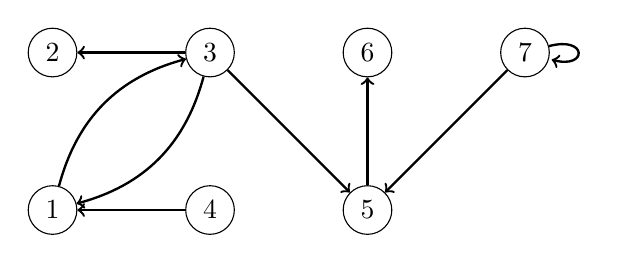
\begin{tikzpicture}[]
 \node[circle,draw=black] (1) at (0,0) {$1$};
 \node[circle,draw=black] (2) at (0,2) {$2$};
 \node[circle,draw=black] (3) at (2,2) {$3$};
 \node[circle,draw=black] (4) at (2,0) {$4$};
 \node[circle,draw=black] (5) at (4,0) {$5$};
 \node[circle,draw=black] (6) at (4,2) {$6$};
 \node[circle,draw=black] (7) at (6,2) {$7$};
		
 \draw[->,line width=0.3mm] (4) edge (1) (3) edge (2) (3) to[bend left] (1) (3) edge (5) (5) edge (6) (7) edge (5);
 \draw[->,line width=0.3mm] (1) to[bend left] (3) (7) edge[loop right] (7);
\end{tikzpicture}
\end{center}
\end{bsp} 

\begin{defn}
Für einen gegebenen Knoten $a \in V$ heißt die Anzahl der Knoten $b \in V$ mit $(a,b) \in A$ der \emph{Ausgangsgrad} von~$a$.
Analog heißt für $b \in V$ die Anzahl der Knoten $a \in V$ mit $(a,b) \in A$ der \emph{Eingangsgrad} von~$b$.
\end{defn} 

\begin{defn}
Sind $D=(V,A)$ und $D'=(V',A')$ zwei Digraphen, so dass $V' \subseteq V$ und $A' \subseteq A$ gelten, so nennt man $D'$ einen \emph{Teilgraphen} von~$D$.
Ist $W \subseteq V$ so heißt
\[
D_{W} := \left( W, \setcond{(a,b)}{a,b \in W \text{ und } (a,b) \in A} \right)
\]
der durch $W$ \emph{induzierte} Teilgraph von~$D$.
\end{defn}

\begin{defn} 
Für einen Digraphen $D=(V,A)$ und Knoten $a,b \in V$ heißt ein Tupel $(v_0,\ldots,v_k)$ mit $(v_i,v_{i+1}) \in A$, für $0 \leq i \leq k-1$ und $v_0=a$ und $v_k=b$ ein \emph{$(a,b)$-Pfad} der Länge~$k$.
Ein Pfad heißt \emph{Weg}, wenn die Knoten des Pfades paarweise verschieden sind.
Der Pfad $(v_i,\ldots,v_j)$ mit $0 \le i \le j \le k$ heißt \emph{Teilpfad} von $(v_0,\ldots,v_k)$.
Ein $(a,b)$-Pfad mit $a=b$ heißt \emph{Zyklus}.
Ein Zyklus $(v_0,\ldots,v_k)$ heißt \emph{Kreis}, falls die Knoten $v_1,\ldots,v_{k-1}$ paarweise verschieden sind.
Die Zyklen $(v_0,\ldots,v_k)$ und $(v_i,\ldots,v_k,v_0,\ldots,v_i)$ werden als gleich angesehen.
Man sagt eine Kante $(u,v)$ \emph{gehört} zu einem Pfad $(v_0,\ldots,v_k)$, falls $u=v_i$ und $v=v_{i+1}$ für ein $i$ mit $0 \le i \leq k-1$ gilt.
Digraphen ohne Zyklen heißen \emph{azyklisch}.
\end{defn} 

%Seien $G=(V,E)$ und $G=(V',E')$ Digraphen und sei $f: V \to V'$ eine Bijektion mit $(a,b) \in E$ $\Leftrightarrow$ $(f(a), f(b)) \in E'$. Die Bijektion $f$ heißt Isomorphismus von $G$ nach $G'$. Zwei Digraphen heißen isomorph, falls ein Isomorphismus von $G$ nach $G'$ existiert. 

\begin{bsp} 
Im Beispieldigraphen von oben markieren wir den Weg $(4,1,3,5,6)$ in blau:

\begin{center}
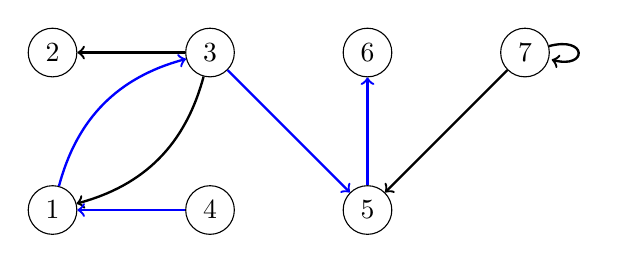
\begin{tikzpicture}[]
 \node[circle,draw=black] (1) at (0,0) {$1$};
 \node[circle,draw=black] (2) at (0,2) {$2$};
 \node[circle,draw=black] (3) at (2,2) {$3$};
 \node[circle,draw=black] (4) at (2,0) {$4$};
 \node[circle,draw=black] (5) at (4,0) {$5$};
 \node[circle,draw=black] (6) at (4,2) {$6$};
 \node[circle,draw=black] (7) at (6,2) {$7$};
		
 \draw[->,line width=0.3mm] (3) edge (2) (3) to[bend left] (1) (7) edge (5);
 \draw[->,line width=0.3mm] (7) edge[loop right] (7);
 \draw[->,line width=0.3mm,blue] (4) edge (1) (1) to[bend left] (3) (3) edge (5) (5) edge (6);
 
\end{tikzpicture}
\end{center}
\end{bsp} 

\begin{bem}
Ein wichtiger Aspekt von Digraphen ist die Orientierung der Kanten, die es ermöglicht zwischen Start- und Endknoten zu unterscheiden.
Wird eine solche Orientierung nicht benötigt, so vereinfachen sich manche Begriffe und wir sprechen anstelle von Digraphen dann von Graphen.
\end{bem} 

\begin{defn} 
Sei dazu $V$ wieder eine endliche Menge und sei $E$ nun eine Teilmenge der ungeordneten Paare $\binom{V}{2}:= \setcond{\{a,b\}}{a, b \in V, a \ne b} $ von Elementen aus~$V$.
Das Paar $G=(V,E)$ heißt \emph{Graph} mit \emph{Knotenmenge} $V$ und \emph{Kantenmenge}~$E$.
Die Elemente von $V$ heißen wieder \emph{Knoten} und die Elemente von $E$ heißen \emph{Kanten} (engl.~\emph{edges}) von~$G$.
Ist $\{a,b\} \in E$ eine Kante, so nennen wir~$a$ und~$b$ ihre \emph{Endknoten}.
Wiederum sagen wir, dass die Knoten $a$ und $b$ \emph{benachbart} und die Kante $\{a,b\}$ \emph{inzident} zu~$a$ und $b$ ist.
\end{defn} 

\begin{bem}
Im Gegensatz zu Digraphen erlaubt die Definition eines Graphen keine Schlingen oder parallele Kanten.
In manchen Literaturquellen lässt man mitunter Mehrfachkanten oder \glqq ungerichtete Schlingen\grqq\ zu und spricht dann von einem \emph{einfachen Graphen} wenn man beides verbietet.
\end{bem}

\begin{defn} 
Für einen Knoten $a \in V$ heißt die Anzahl der Knoten $b \in V$ mit $\{a,b\} \in E$ der \emph{Grad} des Knotens~$a$.
Die Begriffe \emph{(induzierter) Teilgraph}, \emph{Pfad}, \emph{Weg}, \emph{Teilpfad}, \emph{Zyklus} und \emph{Kreis} werden für Graphen analog zu denen für Digraphen definiert.
Ein Graph ohne Zyklen heißt \emph{Wald}.
\end{defn}

\begin{defn} 
Ein Graph $G=(V,E)$ heißt \emph{zusammenhängend}, falls für alle Knoten $a, b \in V$ ein $(a,b)$-Pfad existiert.
Ein zusammenhängender Wald heißt \emph{Baum}.
Die Relation \glqq es existiert ein $(a,b)$-Pfad\grqq\ ist eine Äquivalenzrelation auf den Knoten des Graphen~$G$.
Die Äquivalenzklassen bezüglich dieser Relation heißen \emph{Zusammenhangskomponenten} des Graphen.
Ein Wald ist ein Graph bei dem jede Zusammenhangskomponente ein Baum ist.
\end{defn} 


\begin{bsp}
Die folgende Abbildung zeigt einen Graphen mit zwei Zusammenhangskomponenten:

\begin{center}
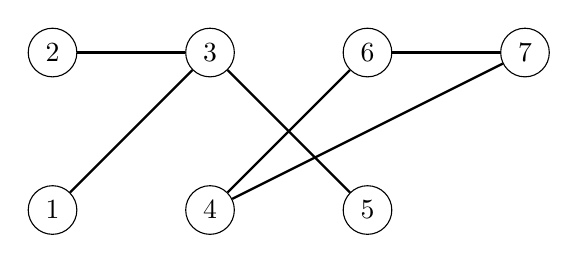
\begin{tikzpicture}[]
 \node[circle,draw=black] (1) at (0,0) {$1$};
 \node[circle,draw=black] (2) at (0,2) {$2$};
 \node[circle,draw=black] (3) at (2,2) {$3$};
 \node[circle,draw=black] (4) at (2,0) {$4$};
 \node[circle,draw=black] (5) at (4,0) {$5$};
 \node[circle,draw=black] (6) at (4,2) {$6$};
 \node[circle,draw=black] (7) at (6,2) {$7$};
		
 \draw[-,line width=0.3mm] (3) edge (2) (3) edge (1) (3) edge (5);
 \draw[-,line width=0.3mm] (4) edge (6) (6) edge (7) (7) edge (4);
\end{tikzpicture}
\end{center}
\end{bsp} 

\begin{bem}
Wir benutzen gelegentlich die Kurzbezeichnung $ab:=(a,b)$ für Kanten von Digraphen und $ab:=\{a,b\}$ für Kanten von Graphen.
Beachten Sie, dass es im Fall einer gerichteten Kante auf die Reihenfolge der Knoten~$a$ und $b$ ankommt.
\end{bem}

\begin{defn}
Ein schleifenfreier Digraph $D = (V,A)$ kann auch als Orientierung eines ungerichteten Graphen $G=(V,E)$ mit $E = \{\{u,v\} : (u,v) \in A\}$ verstanden werden.
Der Graph~$G$ wird dann als der \emph{zugrundeliegende Graph} von~$D$ bezeichnet.
Sobald $E$ nicht leer ist, gibt es stets mindestens zwei Digraphen, denen~$G$ zugrundeliegt.
\end{defn} 

\begin{bsp}
Die folgende Abbildung zeigt einen (schleifenfreien) Digraphen und den dazugehörigen zugrundeliegenden Graphen:
\begin{center}
\hfill
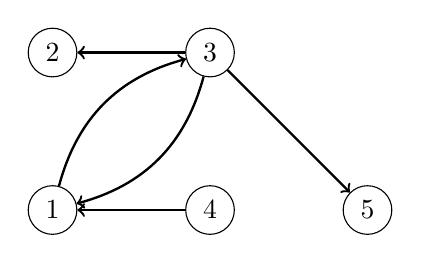
\begin{tikzpicture}[]
 \node[circle,draw=black] (1) at (0,0) {$1$};
 \node[circle,draw=black] (2) at (0,2) {$2$};
 \node[circle,draw=black] (3) at (2,2) {$3$};
 \node[circle,draw=black] (4) at (2,0) {$4$};
 \node[circle,draw=black] (5) at (4,0) {$5$};
		
 \draw[->,line width=0.3mm] (4) edge (1) (3) edge (2) (3) to[bend left] (1) (3) edge (5);
 \draw[->,line width=0.3mm] (1) to[bend left] (3);
\end{tikzpicture}
\hfill
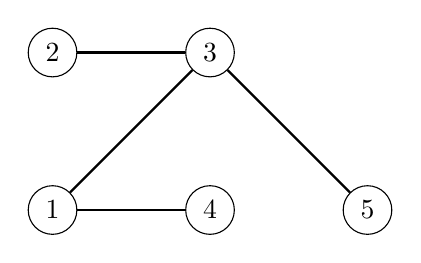
\begin{tikzpicture}[]
 \node[circle,draw=black] (1) at (0,0) {$1$};
 \node[circle,draw=black] (2) at (0,2) {$2$};
 \node[circle,draw=black] (3) at (2,2) {$3$};
 \node[circle,draw=black] (4) at (2,0) {$4$};
 \node[circle,draw=black] (5) at (4,0) {$5$};
		
 \draw[-,line width=0.3mm] (1) edge (4) (3) edge (2) (3) edge (1) (3) edge (5);
\end{tikzpicture}
\hfill\,
\end{center}
Beachten Sie, dass die beiden in entgegengesetzten Richtungen orientierten Kanten zwischen den Knoten $1$ und $3$ zu \emph{einer} Kante im ungerichteten Graphen verschmelzen.
\end{bsp}

\begin{defn} 
Halten wir noch ein paar wichtige spezielle Graphenklassen und deren Bezeichnungen fest: Sei dazu im Folgenden $G=(V,E)$ ein Graph mit $n$ Knoten und $m$ Kanten.
\begin{itemize}
 \item Ist $E=\binom{V}{2}$, so heißt $G$ \emph{vollständig}.
 Ein vollständiger Graph mit $n$ Knoten wird oft mit~$K_n$ bezeichnet.

 \item Ist $E=\emptyset$, so heißt $G$ \emph{leer}.
 Ein leerer Graph mit $n$ Knoten wird oft mit~$\bar K_n$ bezeichnet.

 \item Ist $V$ eine disjunkte Vereinigung zweier Mengen $A$ und $B$ und hat jede Kante von~$G$ die Form $\{a,b\}$ mit $a \in A$ und $b \in B$, so heißt $G$ \emph{bipartit}.
 Die Mengen~$A$ und $B$ heißen dann \emph{Partitionsklassen} von $G$.
 
 \item Ist $G$ bipartit und gilt darüber hinaus, dass jedes $\{a,b\}$ mit $a \in A$ und $b \in B$ eine Kante von $G$ ist, so heißt $G$ \emph{vollständig bipartit}.
 Ein vollständig bipartiter Graph, deren Partitionsklassen die Größe~$r$ und~$s$ haben, wird oft mit~$K_{r,s}$ bezeichnet.
 Natürlich gilt $n = r + s$.
 
 \item Eine \emph{Einbettung} von~$G$ in die Ebene~$\R^2$ ist eine Menge $P=\{p_1,\ldots,p_n\} \subseteq \R^2$ von Punkten zusammen mit einer Menge $S=\{S_1,\ldots,S_m\}$ von Streckensegmenten, so dass es eine Bijektion $f:V \to P$ gibt mit der Eigenschaft, dass $\{u,v\}$ genau dann eine Kante von~$G$ ist, wenn die Punkte $f(u)$ und $f(v)$ Eckpunkte desselben Streckensegmentes~$S_i$ sind.
 Besitzt ein Graph eine Einbettung bei der je zwei verschiedene Streckensegmente sich höchstens in Eckpunkten schneiden, so heißt dieser Graph \emph{planar}.
 
 Beispiele: $K_n$ ist planar genau dann wenn $n\leq4$ ist; $K_{3,3}$ ist nicht planar.
\end{itemize}
\end{defn} 

\begin{bsp}
Die nachfolgende Illustration zeigt zwei Darstellungen des $K_4$:
\begin{center}
\hfill
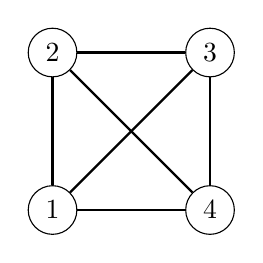
\begin{tikzpicture}[]
\tikzset{every loop/.style={}} % no arrows in loops
 \node[circle,draw=black] (1) at (0,0) {$1$};
 \node[circle,draw=black] (2) at (0,2) {$2$};
 \node[circle,draw=black] (3) at (2,2) {$3$};
 \node[circle,draw=black] (4) at (2,0) {$4$};
		
 \draw[-,line width=0.3mm] (1) edge (2) (1) edge (3) (1) edge (4) (2) edge (3) (2) edge (4) (3) edge (4);
		% (4) edge[loop right] (4);		
\end{tikzpicture}
\hfill
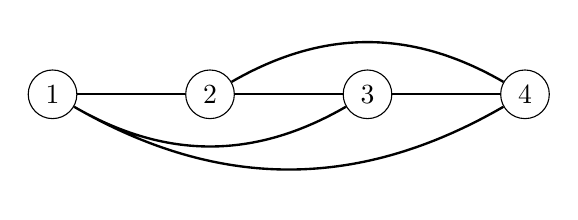
\begin{tikzpicture}[]
\tikzset{every loop/.style={}} % no arrows in loops
 \node[circle,draw=black] (1) at (0,0) {$1$};
 \node[circle,draw=black] (2) at (2,0) {$2$};
 \node[circle,draw=black] (3) at (4,0) {$3$};
 \node[circle,draw=black] (4) at (6,0) {$4$};
		
 \draw[-,line width=0.3mm] (1) edge (2) (2) edge (3) (3) edge (4);
 \draw[-,line width=0.3mm] (1) to[bend right] (3) (1) to[bend right] (4);
 \draw[-,line width=0.3mm] (2) to[bend left] (4);		
\end{tikzpicture}
\hfill\,
\end{center}
Keine der beiden Darstellungen zeigt, dass $K_4$ planar ist.
Warum nicht?
Finden Sie eine Darstellung, die dies illustriert!
\end{bsp}



\begin{bem}
In der Graphentheorie ist die Bezeichnung der Hautbegriffe nicht einheitlich.
Von Quelle zu Quelle unterscheiden sich die Definitionen geringfügig und insbesondere in Bezug auf die Namensgebung gibt es teilweise große Unterschiede.
Zu diesem Zweck listen wir hier die geläufigsten Synonyme um mögliche Verwirrungen beim Lesen unterschiedlicher Quellen zu vermeiden:
\begin{align*}
\text{gerichteter Graph} &= \text{Digraph}\\
\text{Knoten} &= \text{Ecke}\\
\text{gerichtete Kante} &= \text{Bogen}\\
\text{adjazent} &= \text{benachbart}\\
\text{Grad} &= \text{Valenz}\\
\text{Weg} &= \text{einfacher Pfad}\\
\text{Kreis} &= \text{einfacher Zyklus}\\
\text{Kantenzug} &= \text{Pfad}\\
\text{geschlossener Kantenzug} &= \text{Zyklus}\\
\text{Schleife} &= \text{Schlinge}
\end{align*}
\end{bem}

\begin{bem}
Zum Abschluss dieser Einführung in die Grundbegriffe schauen wir uns noch verschiedene Möglichkeiten an, wie man einen gegebenen (Di)Graphen im Rechner darstellt, das heißt, in welcher Form man die Beziehungen zwischen Knoten und (gerichteten) Kanten verwalten kann.

Sei dazu ein Graph oder ein Digraph gegeben und zur Vereinheitlichung im Folgenden mit $G=(V,E)$ bezeichnet.
\end{bem} 

\begin{defn}
{\bfseries Kantenliste:} Liste/Array der Kanten von $G$. 
\end{defn}

\begin{bsp}\ 
\begin{center}
\hfill
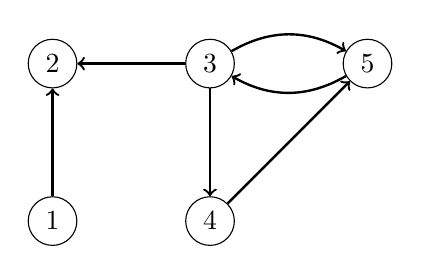
\begin{tikzpicture}[]
 \node[circle,draw=black] (1) at (0,0) {$1$};
 \node[circle,draw=black] (2) at (0,2) {$2$};
 \node[circle,draw=black] (3) at (2,2) {$3$};
 \node[circle,draw=black] (4) at (2,0) {$4$};
 \node[circle,draw=black] (5) at (4,2) {$5$};
% \node[black] (G) at (2,3.5) {$G=(V,E)$};
		
 \draw[->,line width=0.3mm] (1) edge (2) (3) edge (2) (3) edge (4) (3) to[bend left] (5) (4) edge (5);
 \draw[->,line width=0.3mm] (5) to[bend left] (3);
\end{tikzpicture}
\hfill
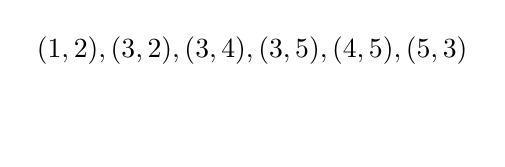
\begin{tikzpicture}[]
 \node[black] (1) at (0,0) {$(1,2),(3,2),(3,4),(3,5),(4,5),(5,3)$};
 \node[black] (1) at (0,-1) {$ $};
\end{tikzpicture}
\hfill\,
\end{center}
\end{bsp}

\begin{defn} 
{\bfseries Adjazenzliste:} Hier speichern wir die Knotenmenge $V$ als Liste und jedem Element $u \in V$ der Liste wird eine Liste aller Knoten $v \in V$ mit $uv \in E$ zugeordnet.
Der Speicherplatzbedarf für diese Darstellung ist offensichtlich $\Theta(|V|+|E|)$.
\end{defn}

\begin{bsp} \ 
\begin{center}
\hfill
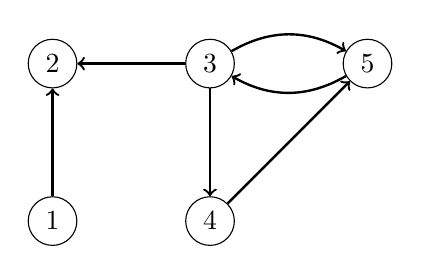
\begin{tikzpicture}[]
 \node[circle,draw=black] (1) at (0,0) {$1$};
 \node[circle,draw=black] (2) at (0,2) {$2$};
 \node[circle,draw=black] (3) at (2,2) {$3$};
 \node[circle,draw=black] (4) at (2,0) {$4$};
 \node[circle,draw=black] (5) at (4,2) {$5$};
% \node[black] (G) at (2,3.5) {$G=(V,E)$};
		
 \draw[->,line width=0.3mm] (1) edge (2) (3) edge (2) (3) edge (4) (3) to[bend left] (5) (4) edge (5);
 \draw[->,line width=0.3mm] (5) to[bend left] (3);
\end{tikzpicture}
\hfill
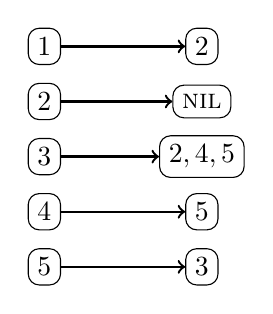
\begin{tikzpicture}[]
 \node[rounded corners,draw=black] (1) at (0,0) {$1$};
 \node[rounded corners,draw=black] (L1) at (2,0) {$2$};
 \node[rounded corners,draw=black] (2) at (0,-.7) {$2$};
 \node[rounded corners,draw=black] (L2) at (2,-.7) {$\textsc{nil}$};
 \node[rounded corners,draw=black] (3) at (0,-1.4) {$3$};
 \node[rounded corners,draw=black] (L3) at (2,-1.4) {$2,4,5$};
 \node[rounded corners,draw=black] (4) at (0,-2.1) {$4$};
 \node[rounded corners,draw=black] (L4) at (2,-2.1) {$5$};
 \node[rounded corners,draw=black] (5) at (0,-2.8) {$5$};
 \node[rounded corners,draw=black] (L5) at (2,-2.8) {$3$};
		
 \draw[->,line width=0.3mm] (1) edge (L1) (2) edge (L2) (3) edge (L3) (4) edge (L4) (5) edge (L5);
\end{tikzpicture}
\hfill\,
\end{center}
\end{bsp} 

\begin{defn} 
{\bfseries Adjazenzmatrix:} Sei $V=\{v_1,\ldots,v_n\}$.
Die Adjazenzmatrix von~$G$ ist die Matrix $A=(a_{i,j}) \in \R^{n \times n}$ mit Einträgen
\[
a_{i,j} = \begin{cases}1&,\text{ falls }\{v_i,v_j\} \in E \text{ bzw.~falls }(v_i,v_j) \in E,\\ 0&,\text{ sonst}.\end{cases}
\]
Der Speicherplatzbedarf (bei direkter Implementierung von Matrizen) ist $\Theta(|V|^2)$.

\begin{center}
\hfill
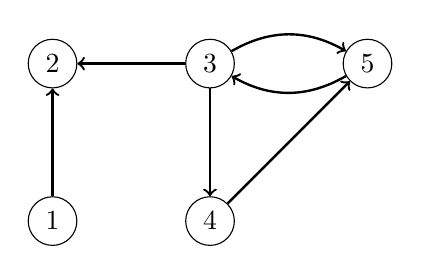
\begin{tikzpicture}[]
 \node[circle,draw=black] (1) at (0,0) {$1$};
 \node[circle,draw=black] (2) at (0,2) {$2$};
 \node[circle,draw=black] (3) at (2,2) {$3$};
 \node[circle,draw=black] (4) at (2,0) {$4$};
 \node[circle,draw=black] (5) at (4,2) {$5$};
% \node[black] (G) at (2,3.5) {$G=(V,E)$};
		
 \draw[->,line width=0.3mm] (1) edge (2) (3) edge (2) (3) edge (4) (3) to[bend left] (5) (4) edge (5);
 \draw[->,line width=0.3mm] (5) to[bend left] (3);
\end{tikzpicture}
\hfill
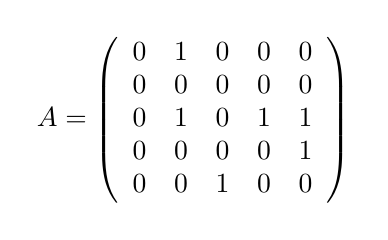
\begin{tikzpicture}[]
 \node[black] (1) at (0,0) {$A=\left(\begin{array}{ccccc}
0 & 1 & 0 & 0 & 0 \\
0 & 0 & 0 & 0 & 0 \\
0 & 1 & 0 & 1 & 1 \\
0 & 0 & 0 & 0 & 1 \\
0 & 0 & 1 & 0 & 0
\end{array}\right)$
};
\end{tikzpicture}
\hfill\,
\end{center}
\end{defn} 

\begin{defn}
{\bfseries Inzidenzmatrix:} Sei $V=\{v_1,\ldots,v_n\}$ und $E=\{e_1,\ldots,e_m\}$.
Sei weiterhin $G$ zunächst als gerichteter Graph ohne Schleifen angenommen.
Die Inzidenzmatrix von~$G$ ist die Matrix $B=(b_{i,j}) \in \R^{n \times m}$ mit Einträgen
\[
b_{i,j} = \begin{cases}1&,\text{ falls }v_i\text{ Startknoten von }e_j\text{ ist},\\ -1&,\text{ falls }v_i\text{ Endknoten von }e_j\text{ ist},\\ 0&,\text{ sonst}.\end{cases}
\]
Ist $G$ ein ungerichteter Graph, so lassen wir lediglich die Vorzeichen weg, das heißt, die Einträge der Inzidenzmatrix sind
\[
b_{i,j} = \begin{cases}1&,\text{ falls }v_i\text{ Endknoten von }e_j\text{ ist},\\ 0&,\text{ sonst}.\end{cases}
\]
Der Speicherplatzbedarf (bei direkter Implementierung von Matrizen) ist $\Theta(|V|\cdot|E|)$.
\end{defn} 

\begin{bsp} \ 
\begin{center}
\hfill
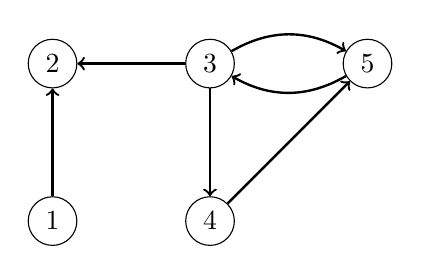
\begin{tikzpicture}[]
 \node[circle,draw=black] (1) at (0,0) {$1$};
 \node[circle,draw=black] (2) at (0,2) {$2$};
 \node[circle,draw=black] (3) at (2,2) {$3$};
 \node[circle,draw=black] (4) at (2,0) {$4$};
 \node[circle,draw=black] (5) at (4,2) {$5$};
% \node[black] (G) at (2,3.5) {$G=(V,E)$};
		
 \draw[->,line width=0.3mm] (1) edge (2) (3) edge (2) (3) edge (4) (3) to[bend left] (5) (4) edge (5);
 \draw[->,line width=0.3mm] (5) to[bend left] (3);
\end{tikzpicture}
\hfill
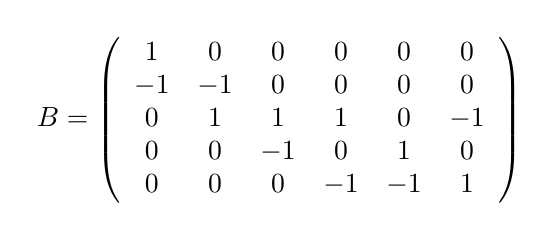
\begin{tikzpicture}[]
 \node[black] (1) at (0,0) {$B=\left(\begin{array}{cccccc}
1 & 0 & 0 & 0 & 0 & 0\\
-1 & -1 & 0 & 0 & 0 & 0\\
0 & 1 & 1 & 1 & 0 & -1\\
0 & 0 & -1 & 0 & 1 & 0\\
0 & 0 & 0 & -1 & -1 & 1
\end{array}\right)$
};
\end{tikzpicture}
\hfill\,
\end{center}

Die Kanten in der vorigen Abbildung sind in der Reihenfolge $12,32,34,35,45,53$ nummeriert.
\end{bsp}  
\section{Breitensuche}


\begin{bem}
Die Eingabe für die Breitensuche ist ein Digraph $D=(V,A)$ in Form einer \underline{Adjazenzliste}~$N$.
Das heißt, für jeden Knoten $u \in V$ ist $N[u]$ eine Liste aller $v \in V$ mit $(u,v) \in A$.
%Wie wir sehen werden erlaubt die Darstellung von $D$ als Adjazenzliste eine Durchmusterung mit der optimalen Laufzeit $\Theta(|V|+|A|)$.
Erinnern Sie sich, dass der Speicherplatz für die Adjazenzliste $\Theta(|V|+|A|)$ beträgt.

Auf ungerichteten Graphen ist die Vorgehensweise analog und wir diskutieren (fast ausschließlich) die gerichtete Variante.
\end{bem}


\begin{bem} 
\underline{Die Idee der Breitensuche:} (engl.~\textbf{breadth first search}, daher auch kurz BFS genannt).

Die Breitensuche ist ein \glqq vorsichtiger\grqq\ Erkundungs-Algorithmus zur Durchmusterung von Graphen.
Wir fassen die Knoten $u \in V$ als Orte und $N[u]$ als die Nachbarschaft des Ortes~$u$ auf.
Die Breitensuche will zuerst die gesamte Nachbarschaft eines Ortes erkunden, bevor sie sich \glqq traut\grqq\ weiter in die Welt hinauszugehen:
\begin{itemize} 
 \item Man sucht die Umgebung von $u$ durch. 
 \item Man erkundet erst die Nachbarschaft eines zuvor noch nicht gesehenen Ortes~$v$, wenn man alle Orte gesehen hat, die man von $u$ aus erreichen kann. 
\end{itemize} 
%
Die Umsetzung dieser Strategie basiert auf Farbattributen der Knoten, die man im Laufe der Durchmusterung sukzessiv zuerst als weiß ($=$ noch nicht gesehen), dann als grau ($=$ gesehen aber noch nicht abgearbeitet) und schließlich als schwarz ($=$ abgearbeitet) setzt. 
\end{bem}


\begin{defn}
Wenn die Breitensuche entlang einer Kante verläuft, die in einen weißen Knoten endet, dann sagen wir, dass der entsprechende Knoten \textbf{entdeckt} wird.

\noindent Eine Zusammenfassung der Bedeutung der Farben der Knoten:
\begin{itemize}
	\item[] {\bfseries weiß:} Der Knoten wurde noch nicht entdeckt. 
	\item[] {\bfseries grau:} Der Knoten wurde entdeckt und die Breitensuche für den Knoten läuft gerade.
	\item[] {\bfseries schwarz:} Der Knoten wurde entdeckt und die Breitensuche für den Knoten ist bereits beendet.
\end{itemize}

\noindent Wird ein Knoten schwarz gefärbt, so sagen wir auch dass er \textbf{abgearbeitet} wurde.
\end{defn}


\begin{defn}
Für zwei Knoten $u,v \in V$ in~$D$ definieren wir den \textbf{Abstand} (die \textbf{Distanz}) von~$u$ nach~$v$ als die minimale Länge eines $(u,v)$-Pfades und bezeichnen ihn mit $\delta(u,v)$.
Wenn kein solcher Pfad existiert, setzen wir $\delta(u,v):=\infty$.
Für ungerichtete Graphen ist $\delta(u,v)$ entsprechend definiert und es gilt $\delta(u,v)=\delta(v,u)$ für alle Knoten $u,v \in V$.
Gilt für einen Knoten $s \in V$, dass $\delta(s,v) < \infty$, so sagen wir, dass~$v$ von~$s$ aus \textbf{erreichbar} ist.
\end{defn} 

\begin{bem} 
Die Breitensuche erlaubt das Bestimmen der Abstände $\delta(s,v)$ von einem festen \textbf{Startknoten} $s \in V$ aus zu jedem anderen Knoten~$v \in V$.

Während der Durchmusterung des Digraphen~$D=(V,A)$ wird dabei ein Array~$d$ der Länge~$|V|$ verwaltet, in dem nach Abschluss der Breitensuche die Abstände $\delta(s,v)$, für alle Knoten $v \in V$, gespeichert sind.
\end{bem} 


\begin{bem} 
Vor der eigentlichen Breitensuche müssen eine Reihe von Attributen korrekt initialisiert werden:
\begin{itemize}
 \item Zu Beginn setzen wir $d[v]:=\infty$, für alle $v \in V \setminus \{s\}$, und $d[s]:=0$.
Besteht die Gleichheit $d[v]=\infty$ zu einem Moment der Breitensuche, so bedeutet dies, dass der Knoten~$v$ bisher noch nicht entdeckt wurde.
Die erste Veränderung des Wertes~$d[v]$ entspricht der Entdeckung von~$v$, und wir nennen $d[v]$ die \textbf{aktuelle Distanz} von~$s$ zu~$v$. 
 \item Wir verwalten weiterhin ein \textbf{Farbattribut} $\cc{Farbe}[u]$ für jeden Knoten~$u \in V$ um den Bearbeitungszustand von~$u$ zu jedem Zeitpunkt der Breitensuche zu kennen.
 \item Desweiteren kommt die sogenannte \textbf{Vorgängerabbildung}~$\pi$ zum Einsatz.
 Dies ist ein Array~$\pi$ mit $|V|$ Komponenten.
	Durch $\pi[v]$ wird notiert von welchem Knoten aus der Knoten $v$ entdeckt wurde.
\end{itemize}
\end{bem} 

%\begin{defn}
%	Die \textbf{Vorgängerabbildung} ist ein Array~$\pi$ mit $|V|$ Komponenten.
%	Durch $\pi[v]$ wird notiert von welchem Knoten aus der Knoten $v$ entdeckt wurde.
%\end{defn}

\begin{defn} 
Für die Umsetzung der Breitensuche wird die folgende Hilfsdatenstruktur benutzt.
Eine \textbf{Warteschlange}~$Q$ ist eine Liste $Q=[q_1,\ldots,q_k]$, die mit zwei Grundoperationen ausgestattet ist:
\begin{itemize}
 \item $\cc{Dequeue}(Q)$: Das \textbf{erste} Element~$q_1$ von~$Q$ wird zurückgegeben und aus der Warteschlange entfernt.
 Man nennt das Element~$q_1$ den \textbf{Kopf} der Warteschlange und nach der Operation gilt $Q=[q_2,\ldots,q_k]$.

 \item $\cc{Enqueue}(Q,x)$: Das Element~$x$ wird am \textbf{Ende} von~$Q$ hinzugefügt.
 Nach Ausführung dieser Operation gilt also $Q=[q_1,\ldots,q_k,x]$. 
\end{itemize}
\end{defn} 

\begin{bem}
Aufgrund der Einfüge- und Rückgabereihenfolge sagt man auch, dass Warteschlangen nach dem FIFO-Prinzip (First In - First Out) arbeiten.
Warteschlangen mit höchstens $n \in \N$ Elementen können auf der Basis von Arrays der Länge~$n$ umgesetzt werden, sodass die Laufzeit der beiden Grundoperationen $\Theta(1)$ Zeiteinheiten beträgt. 
\end{bem} 



\begin{bem} 
Auch die Warteschlange muss korrekt initialisiert werden.
Wir fassen alle Initialisierungen zu einer eigenen Hilfsprozedur zusammen:

\begin{algorithm}[H]
\caption{$\cc{Breitensuche-initialisieren}(s)$}
\begin{algorithmic}[1]
 \FOR{$u \in V \setminus \{s\}$}
  \STATE $\cc{Farbe}[u] := \cc{weiss}$
  \STATE $d[u] := \infty$ $\quad$ \COMMENT{Aktueller Abstand zu $s$}
  \STATE $\pi[u] := \cc{nil}$ $\quad$ \COMMENT{Vorgänger von $u$}
 \ENDFOR
 \STATE $\cc{Farbe}[s] := \cc{grau}$
 \STATE $d[s] := 0$
 \STATE $\pi[s] := \cc{nil}$
 \STATE Deklariere eine leere Warteschlange $Q$
 \STATE $\cc{Enqueue}(Q,s)$
\end{algorithmic}
\end{algorithm}
\end{bem}

\begin{bem}
Die Breitensuche ist so umgesetzt, dass das \glqq Leben\grqq\ eines jeden Knotens $u$ als der folgende Ablauf zusammengefasst werden kann: 
\begin{equation*}
	\cc{weiss} 
	\ \xrightarrow{\text{$u$ kommt in $Q$}} \ 
	\cc{grau}
	\  \xrightarrow{\text{$u$ verlässt $Q$}} \ 
	\ \xrightarrow{\text{Sondierung von $N[u]$}} \ 
	\cc{schwarz} 
\end{equation*} 
%
Beim Sondieren/Erkunden der Nachbarschaft $N[u]$ von~$u$ werden weiße Knoten entdeckt: Sie werden in $Q$ eingefügt und dann grau gefärbt. Die Breitensuche ist durch die Wahl des Containers~$Q$ als \underline{Warteschlange} ausgezeichnet.

Durch diese Wahl \glqq simuliert\grqq\ die Breitensuche die Ausbreitung einer Welle in einem Medium. Stellen Sie sich vor in $s$ kommt es zu einer Explosion; die Schallwelle breitet sich im Graphen $D$ entlang der Kanten aus und erreicht mit der Zeit immer mehr Knoten. Wie sich die Front der Schallwelle durch die Knoten ausbreitet wird durch die Warteschlange $Q$ \glqq modelliert\grqq.


\begin{algorithm}[H]
\caption{$\cc{Breitensuche}(s)$}
\begin{algorithmic}[1]
 \STATE $\cc{Breitensuche-initialisieren}(s)$
 \WHILE{$Q$ enthält Knoten}
  \STATE\label{line:breitensuche-dequeue} $u:=\cc{Dequeue}(Q)$ $\quad$ \COMMENT{Die Bearbeitung des Knotens $u$ beginnt.}
  \STATE \COMMENT{Aus $u$ ausgehende Kanten werden sondiert/untersucht}
  \FOR{$v \in N[u]$}
   \IF{$\cc{Farbe}[v]=\cc{weiss}$}\label{line:breitensuche-if}
    \STATE $\cc{Farbe}[v]:=\cc{grau}$
    \STATE\label{line:breitensuche-enqueue} $\cc{Enqueue}(Q,v)$
    \STATE\label{line:breitensuche-pi} $\pi[v] := u$
    \STATE\label{line:breitensuche-d} $d[v]:=d[u]+1$
   \ENDIF
  \ENDFOR
  \STATE $\cc{Farbe}[u]:=\cc{schwarz}$
 \ENDWHILE
\end{algorithmic}
\end{algorithm}
\end{bem}

\begin{bem}\ Hier eine Umsetzung der BFS in Sage/Python: 
\lstinputlisting[language=Python]{Code/bfs.sage}
\end{bem} 

\begin{bsp}
\label{bsp:breitensuche}
Wir sehen uns die Arbeitsweise der Breitensuche auf dem folgenden Digraphen an:

\condclearpage 
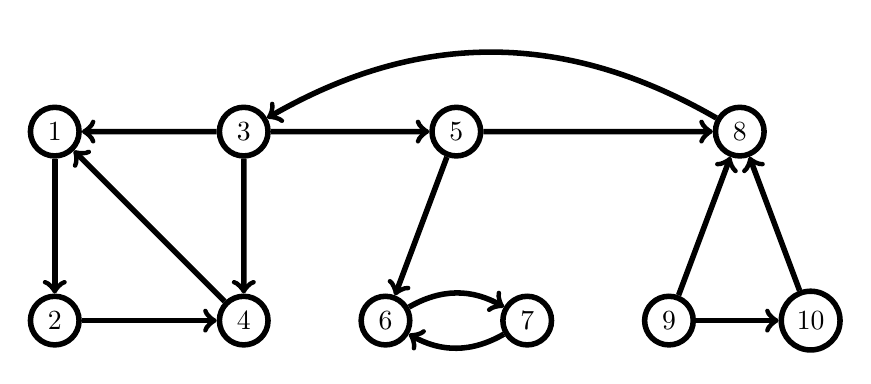
\begin{tikzpicture}[line width=2,scale=1.2]
 \node[circle,draw=black] (1) at (0,2) {$1$};
 \node[circle,draw=black] (2) at (0,0) {$2$};
 \node[circle,draw=black] (3) at (2,2) {$3$};
 \node[circle,draw=black] (4) at (2,0) {$4$};
 \node[circle,draw=black] (5) at (4.25,2) {$5$};
 \node[circle,draw=black] (6) at (3.5,0) {$6$};
 \node[circle,draw=black] (7) at (5,0) {$7$};
 \node[circle,draw=black] (8) at (7.25,2) {$8$};
 \node[circle,draw=black] (9) at (6.5,0) {$9$};
 \node[circle,draw=black] (10) at (8,0) {$10$};
		
 \draw[->] (1) edge (2);
 \draw[->] (2) edge (4);
 \draw[->] (3) edge (1) (3) edge (4) (3) edge (5);
 \draw[->] (4) edge (1);
 \draw[->] (5) edge (6) (5) edge (8); 
 \draw[->] (6) to[bend left] (7);
 \draw[->] (7) to[bend left] (6);
 \draw[->] (8) to[bend right] (3);
 \draw[->] (9) edge (8) (9) edge (10);
 \draw[->] (10) edge (8); 
\end{tikzpicture}
\hfill\,

Als Startknoten wählen wir~$s=3$ und treffen ansonsten jede Wahl aufsteigend in der Reihenfolge der Knotenindizes.
Wir zeigen die ersten 8 Schritte durch die folgende Sequenz von gefärbten Digraphen.
Dabei entspricht die Knotenfarbe dem aktuellen Farbattribut und die bereits sondierten Kanten sind rot markiert:

\condclearpage 
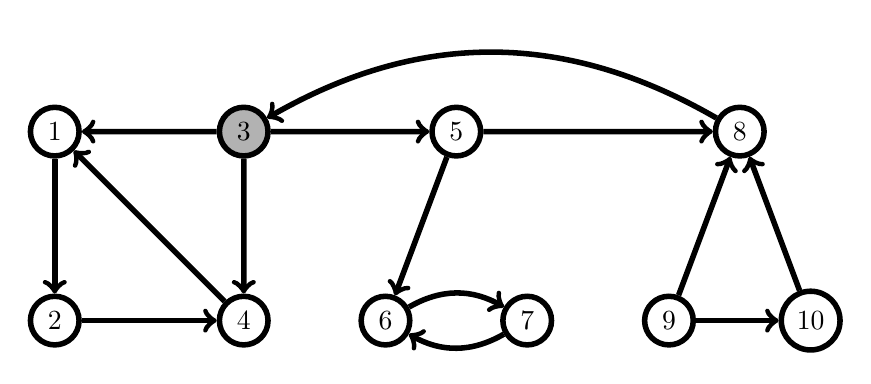
\begin{tikzpicture}[line width=2,scale=1.2]
 \tikzset{gnode/.style ={fill=black!30!,circle,draw}}
 \tikzset{snode/.style ={white,fill=black,circle,draw}}

 \node[circle,draw=black] (1) at (0,2) {$1$};
 \node[circle,draw=black] (2) at (0,0) {$2$};
 \node[gnode] (3) at (2,2) {$3$};
 \node[circle,draw=black] (4) at (2,0) {$4$};
 \node[circle,draw=black] (5) at (4.25,2) {$5$};
 \node[circle,draw=black] (6) at (3.5,0) {$6$};
 \node[circle,draw=black] (7) at (5,0) {$7$};
 \node[circle,draw=black] (8) at (7.25,2) {$8$};
 \node[circle,draw=black] (9) at (6.5,0) {$9$};
 \node[circle,draw=black] (10) at (8,0) {$10$};
		
 \draw[->] (1) edge (2);
 \draw[->] (2) edge (4);
 \draw[->] (3) edge (1) (3) edge (4) (3) edge (5);
 \draw[->] (4) edge (1);
 \draw[->] (5) edge (6) (5) edge (8); 
 \draw[->] (6) to[bend left] (7);
 \draw[->] (7) to[bend left] (6);
 \draw[->] (8) to[bend right] (3);
 \draw[->] (9) edge (8) (9) edge (10);
 \draw[->] (10) edge (8); 
\end{tikzpicture}
\hfill\, $Q: \ 3 $

\condclearpage 
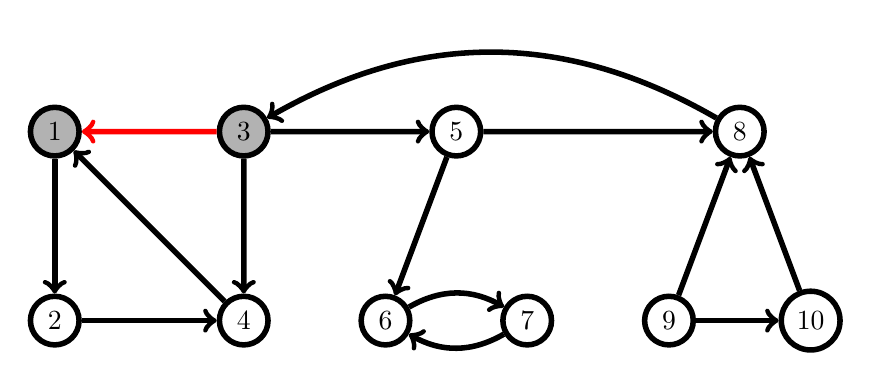
\begin{tikzpicture}[line width=2,scale=1.2]
 \tikzset{gnode/.style ={fill=black!30!,circle,draw}}
 \tikzset{snode/.style ={white,fill=black,circle,draw}}

 \node[gnode] (1) at (0,2) {$1$};
 \node[circle,draw=black] (2) at (0,0) {$2$};
 \node[gnode] (3) at (2,2) {$3$};
 \node[circle,draw=black] (4) at (2,0) {$4$};
 \node[circle,draw=black] (5) at (4.25,2) {$5$};
 \node[circle,draw=black] (6) at (3.5,0) {$6$};
 \node[circle,draw=black] (7) at (5,0) {$7$};
 \node[circle,draw=black] (8) at (7.25,2) {$8$};
 \node[circle,draw=black] (9) at (6.5,0) {$9$};
 \node[circle,draw=black] (10) at (8,0) {$10$};
		
 \draw[->] (1) edge (2);
 \draw[->] (2) edge (4);
 \draw[->,red] (3) edge (1);
 \draw[->] (3) edge (4) (3) edge (5);
 \draw[->] (4) edge (1);
 \draw[->] (5) edge (6) (5) edge (8); 
 \draw[->] (6) to[bend left] (7);
 \draw[->] (7) to[bend left] (6);
 \draw[->] (8) to[bend right] (3);
 \draw[->] (9) edge (8) (9) edge (10);
 \draw[->] (10) edge (8); 
\end{tikzpicture}
\hfill\, $Q: \ \not 3\ 1 $ 

\condclearpage 
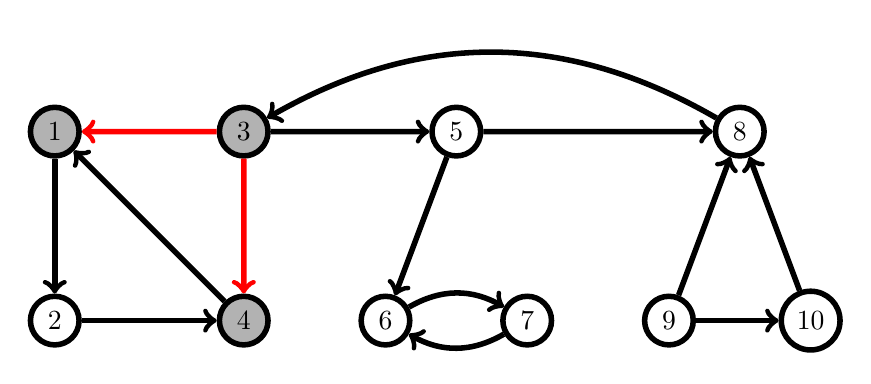
\begin{tikzpicture}[line width=2,scale=1.2]
 \tikzset{gnode/.style ={fill=black!30!,circle,draw}}
 \tikzset{snode/.style ={white,fill=black,circle,draw}}

 \node[gnode] (1) at (0,2) {$1$};
 \node[circle,draw=black] (2) at (0,0) {$2$};
 \node[gnode] (3) at (2,2) {$3$};
 \node[gnode] (4) at (2,0) {$4$};
 \node[circle,draw=black] (5) at (4.25,2) {$5$};
 \node[circle,draw=black] (6) at (3.5,0) {$6$};
 \node[circle,draw=black] (7) at (5,0) {$7$};
 \node[circle,draw=black] (8) at (7.25,2) {$8$};
 \node[circle,draw=black] (9) at (6.5,0) {$9$};
 \node[circle,draw=black] (10) at (8,0) {$10$};
		
 \draw[->] (1) edge (2);
 \draw[->] (2) edge (4);
 \draw[->,red] (3) edge (1);
 \draw[->,red] (3) edge (4);
 \draw[->] (3) edge (5);
 \draw[->] (4) edge (1);
 \draw[->] (5) edge (6) (5) edge (8); 
 \draw[->] (6) to[bend left] (7);
 \draw[->] (7) to[bend left] (6);
 \draw[->] (8) to[bend right] (3);
 \draw[->] (9) edge (8) (9) edge (10);
 \draw[->] (10) edge (8); 
\end{tikzpicture}
\hfill\, $Q: \ \not 3\ 1\ 4$ 

\condclearpage 
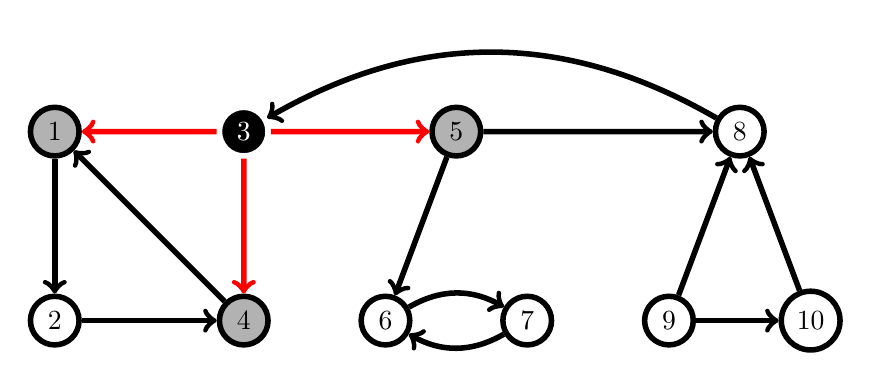
\begin{tikzpicture}[line width=2,scale=1.2]
 \tikzset{gnode/.style ={fill=black!30!,circle,draw}}
 \tikzset{snode/.style ={white,fill=black,circle,draw}}

 \node[gnode] (1) at (0,2) {$1$};
 \node[circle,draw=black] (2) at (0,0) {$2$};
 \node[snode] (3) at (2,2) {$3$};
 \node[gnode] (4) at (2,0) {$4$};
 \node[gnode] (5) at (4.25,2) {$5$};
 \node[circle,draw=black] (6) at (3.5,0) {$6$};
 \node[circle,draw=black] (7) at (5,0) {$7$};
 \node[circle,draw=black] (8) at (7.25,2) {$8$};
 \node[circle,draw=black] (9) at (6.5,0) {$9$};
 \node[circle,draw=black] (10) at (8,0) {$10$};
		
 \draw[->] (1) edge (2);
 \draw[->] (2) edge (4);
 \draw[->,red] (3) edge (1);
 \draw[->,red] (3) edge (4);
 \draw[->,red] (3) edge (5);
 \draw[->] (4) edge (1);
 \draw[->] (5) edge (6) (5) edge (8); 
 \draw[->] (6) to[bend left] (7);
 \draw[->] (7) to[bend left] (6);
 \draw[->] (8) to[bend right] (3);
 \draw[->] (9) edge (8) (9) edge (10);
 \draw[->] (10) edge (8); 
\end{tikzpicture}
\hfill\, $Q: \ \not 3\ 1\ 4\ 5$ 

\condclearpage 
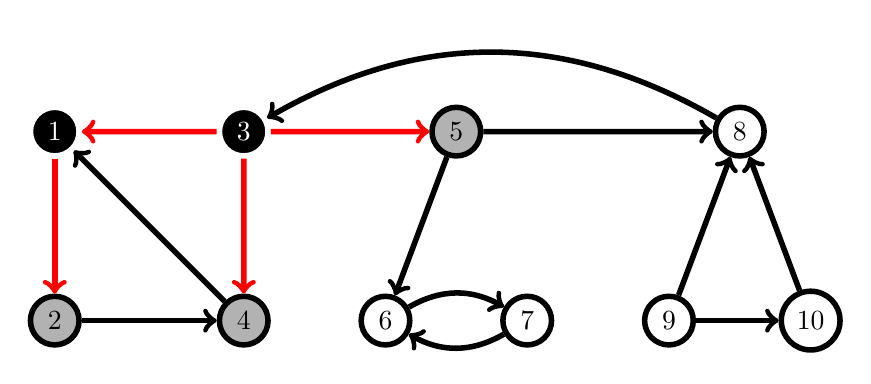
\begin{tikzpicture}[line width=2,scale=1.2]
 \tikzset{gnode/.style ={fill=black!30!,circle,draw}}
 \tikzset{snode/.style ={white,fill=black,circle,draw}}

 \node[snode] (1) at (0,2) {$1$};
 \node[gnode] (2) at (0,0) {$2$};
 \node[snode] (3) at (2,2) {$3$};
 \node[gnode] (4) at (2,0) {$4$};
 \node[gnode] (5) at (4.25,2) {$5$};
 \node[circle,draw=black] (6) at (3.5,0) {$6$};
 \node[circle,draw=black] (7) at (5,0) {$7$};
 \node[circle,draw=black] (8) at (7.25,2) {$8$};
 \node[circle,draw=black] (9) at (6.5,0) {$9$};
 \node[circle,draw=black] (10) at (8,0) {$10$};
		
 \draw[->,red] (1) edge (2);
 \draw[->] (2) edge (4);
 \draw[->,red] (3) edge (1);
 \draw[->,red] (3) edge (4);
 \draw[->,red] (3) edge (5);
 \draw[->] (4) edge (1);
 \draw[->] (5) edge (6) (5) edge (8); 
 \draw[->] (6) to[bend left] (7);
 \draw[->] (7) to[bend left] (6);
 \draw[->] (8) to[bend right] (3);
 \draw[->] (9) edge (8) (9) edge (10);
 \draw[->] (10) edge (8); 
\end{tikzpicture}
\hfill\, $Q: \ \not 3 \not 1\ 4\ 5\ 2$ 

\condclearpage 
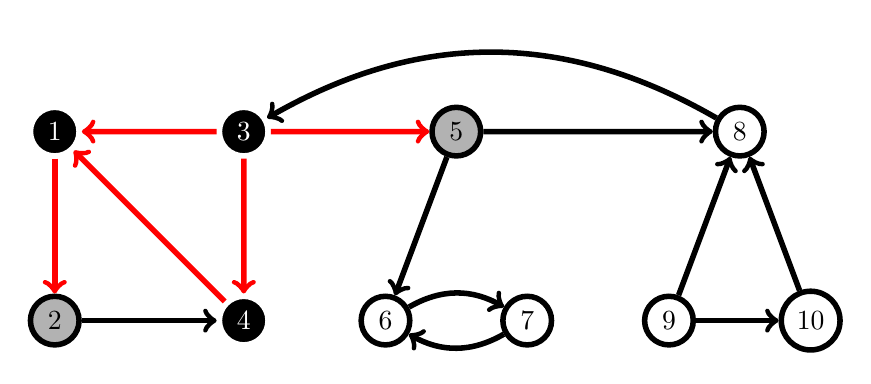
\begin{tikzpicture}[line width=2,scale=1.2]
 \tikzset{gnode/.style ={fill=black!30!,circle,draw}}
 \tikzset{snode/.style ={white,fill=black,circle,draw}}

 \node[snode] (1) at (0,2) {$1$};
 \node[gnode] (2) at (0,0) {$2$};
 \node[snode] (3) at (2,2) {$3$};
 \node[snode] (4) at (2,0) {$4$};
 \node[gnode] (5) at (4.25,2) {$5$};
 \node[circle,draw=black] (6) at (3.5,0) {$6$};
 \node[circle,draw=black] (7) at (5,0) {$7$};
 \node[circle,draw=black] (8) at (7.25,2) {$8$};
 \node[circle,draw=black] (9) at (6.5,0) {$9$};
 \node[circle,draw=black] (10) at (8,0) {$10$};
		
 \draw[->,red] (1) edge (2);
 \draw[->] (2) edge (4);
 \draw[->,red] (3) edge (1);
 \draw[->,red] (3) edge (4);
 \draw[->,red] (3) edge (5);
 \draw[->,red] (4) edge (1);
 \draw[->] (5) edge (6) (5) edge (8); 
 \draw[->] (6) to[bend left] (7);
 \draw[->] (7) to[bend left] (6);
 \draw[->] (8) to[bend right] (3);
 \draw[->] (9) edge (8) (9) edge (10);
 \draw[->] (10) edge (8); 
\end{tikzpicture}
\hfill\, $Q: \ \not 3 \not 1 \not 4\ 5\ 2$

\condclearpage 
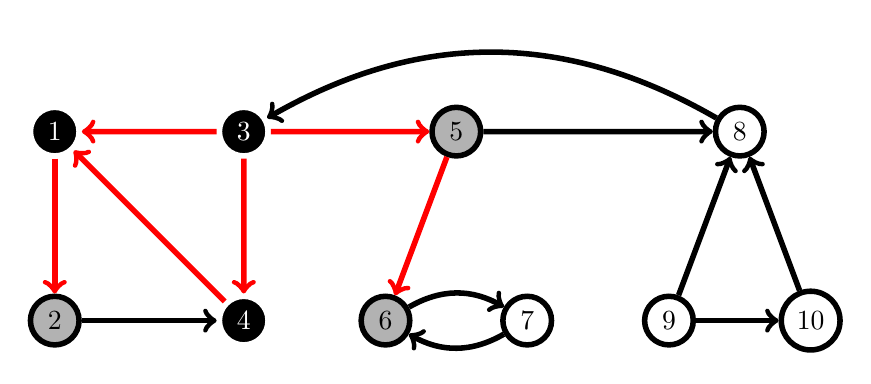
\begin{tikzpicture}[line width=2,scale=1.2]
 \tikzset{gnode/.style ={fill=black!30!,circle,draw}}
 \tikzset{snode/.style ={white,fill=black,circle,draw}}

 \node[snode] (1) at (0,2) {$1$};
 \node[gnode] (2) at (0,0) {$2$};
 \node[snode] (3) at (2,2) {$3$};
 \node[snode] (4) at (2,0) {$4$};
 \node[gnode] (5) at (4.25,2) {$5$};
 \node[gnode] (6) at (3.5,0) {$6$};
 \node[circle,draw=black] (7) at (5,0) {$7$};
 \node[circle,draw=black] (8) at (7.25,2) {$8$};
 \node[circle,draw=black] (9) at (6.5,0) {$9$};
 \node[circle,draw=black] (10) at (8,0) {$10$};
		
 \draw[->,red] (1) edge (2);
 \draw[->] (2) edge (4);
 \draw[->,red] (3) edge (1);
 \draw[->,red] (3) edge (4);
 \draw[->,red] (3) edge (5);
 \draw[->,red] (4) edge (1);
 \draw[->,red] (5) edge (6);
 \draw[->] (5) edge (8); 
 \draw[->] (6) to[bend left] (7);
 \draw[->] (7) to[bend left] (6);
 \draw[->] (8) to[bend right] (3);
 \draw[->] (9) edge (8) (9) edge (10);
 \draw[->] (10) edge (8); 
\end{tikzpicture}
\hfill\, $Q: \ \not 3 \not 1 \not 4 \not 5\ 2\ 6$

\condclearpage 
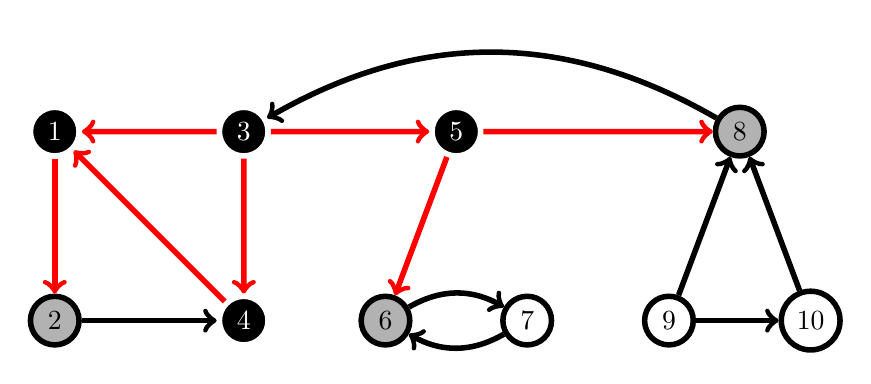
\begin{tikzpicture}[line width=2,scale=1.2]
 \tikzset{gnode/.style ={fill=black!30!,circle,draw}}
 \tikzset{snode/.style ={white,fill=black,circle,draw}}

 \node[snode] (1) at (0,2) {$1$};
 \node[gnode] (2) at (0,0) {$2$};
 \node[snode] (3) at (2,2) {$3$};
 \node[snode] (4) at (2,0) {$4$};
 \node[snode] (5) at (4.25,2) {$5$};
 \node[gnode] (6) at (3.5,0) {$6$};
 \node[circle,draw=black] (7) at (5,0) {$7$};
 \node[gnode] (8) at (7.25,2) {$8$};
 \node[circle,draw=black] (9) at (6.5,0) {$9$};
 \node[circle,draw=black] (10) at (8,0) {$10$};
		
 \draw[->,red] (1) edge (2);
 \draw[->] (2) edge (4);
 \draw[->,red] (3) edge (1);
 \draw[->,red] (3) edge (4);
 \draw[->,red] (3) edge (5);
 \draw[->,red] (4) edge (1);
 \draw[->,red] (5) edge (6) (5) edge (8); 
 \draw[->] (6) to[bend left] (7);
 \draw[->] (7) to[bend left] (6);
 \draw[->] (8) to[bend right] (3);
 \draw[->] (9) edge (8) (9) edge (10);
 \draw[->] (10) edge (8); 
\end{tikzpicture}
\hfill\, $Q: \ \not 3 \not 1 \not 4 \not 5\ 2\ 6\ 8$

\condclearpage 
Da die Knoten~$9$ und~$10$ nicht vom Startknoten $s=3$ aus erreichbar sind, ist der Endzustand nach dem Abschluss von $\cc{Breitensuche}(3)$ der folgende:

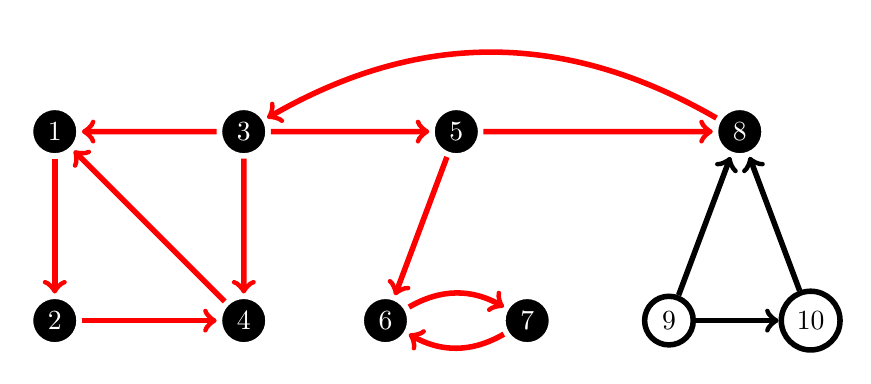
\begin{tikzpicture}[line width=2,scale=1.2]
 \tikzset{gnode/.style ={fill=black!30!,circle,draw}}
 \tikzset{snode/.style ={white,fill=black,circle,draw}}

 \node[snode] (1) at (0,2) {$1$};
 \node[snode] (2) at (0,0) {$2$};
 \node[snode] (3) at (2,2) {$3$};
 \node[snode] (4) at (2,0) {$4$};
 \node[snode] (5) at (4.25,2) {$5$};
 \node[snode] (6) at (3.5,0) {$6$};
 \node[snode] (7) at (5,0) {$7$};
 \node[snode] (8) at (7.25,2) {$8$};
 \node[circle,draw=black] (9) at (6.5,0) {$9$};
 \node[circle,draw=black] (10) at (8,0) {$10$};
		
 \draw[->,red] (1) edge (2);
 \draw[->,red] (2) edge (4);
 \draw[->,red] (3) edge (1);
 \draw[->,red] (3) edge (4) (3) edge (5);
 \draw[->,red] (4) edge (1);
 \draw[->,red] (5) edge (6) (5) edge (8); 
 \draw[->,red] (6) to[bend left] (7);
 \draw[->,red] (7) to[bend left] (6);
 \draw[->,red] (8) to[bend right] (3);
 \draw[->] (9) edge (8) (9) edge (10);
 \draw[->] (10) edge (8); 
\end{tikzpicture}
\hfill\, $Q: \ \not 3 \not1 \not4 \not5 \not2 \not6 \not8 \not7$

\condclearpage 
Weitere Beispiele können mit \verb#bfs_demo.sage# generiert werden.
\end{bsp}

\begin{bem}
Der Beweis der Korrektheit der Breitensuche inklusive der korrekten Bestimmung der Abstände $\delta(s,v)$, für $v \in V$, erfordert noch etwas Vorbereitung.
Die Laufzeitanalyse können wir allerdings bereits durchführen, mit dem Ergebnis, dass die Breitensuche einen optimalen linearen Aufwand $\Theta(|V|+|A|)$ auf einem Digraphen $D  = (V,A)$ erfordert:
\end{bem}

\begin{thm}
\label{thm:laufzeit-breitensuche}
Es sei ein Digraph $D=(V,A)$ durch eine Adjazenzliste gegeben und es sei $s \in V$ ein beliebiger Startknoten.
Die Laufzeit von $\cc{Breitensuche}(s)$ ist $\Theta(|V|+|A|)$.
\end{thm}

\begin{proof}
Der Aufwand für die Initialisierung $\cc{Breitensuche-initialisieren}(s)$ ist direkt als $\Theta(|V|)$ festzustellen. Der Aufwand von $\cc{Breitensuche}(s)$ kann aus dem Diagramm zur Bearbeitung eines Knotens $u \in V$ abgelesen werden: 
\begin{equation*}
	\cc{weiss} 
	\ \xrightarrow{\text{$u$ kommt in $Q$}} \ 
	 \cc{grau}
	 \  \xrightarrow{\text{$u$ verlässt $Q$}} \ 
	 \ \xrightarrow{\text{Sondierung von $N[u]$}}
	\ \cc{schwarz} 
\end{equation*} 
Der Aufwand pro Knoten, der entdeckt wird ist konstant: der Aufwand  besteht aus der Aufnahme in $Q$,  der Färbung von Weiß zu Grau und von Grau zu Schwarz. Der Aufwand pro Kante $(u,v)$, die sondiert wird, ist ebenfalls konstant: jede Kante $(u,v)$ wird höchstens ein Mal sondiert, denn die Sondierung erfolgt nach der Entfernung von $u$ aus der Warteschlange. Nach der Entfernung von $u$ wird $u$ schwarz gefärbt und daher nicht noch einmal in $Q$ aufgenommen. 

Zusammenfassend erhalten wir also  wie behauptet einen Zeitaufwand von
\[
\Theta(|V|) + \Theta(|V|) + \Theta(|A|) = \Theta(|V|+|A|).
\]
\end{proof}


\begin{defn}
Wir nennen einen $(s,v)$-Pfad der Länge $\delta(s,v)$ einen \textbf{kürzesten Pfad} von~$s$ nach~$v$ in~$D$.
\end{defn}

\begin{lem}
\label{lem:breitensuche-pfad-dreieck}
Sei $D=(V,A)$ ein Digraph und sei $s \in V$ ein beliebiger Startknoten.
Dann  gilt für jede Kante $(u,v) \in A$, dass
\[
\delta(s,v) \leq \delta(s,u) + 1.
\]
\end{lem}

\begin{proof}
Falls $u$ von $s$ aus erreichbar ist, dann ist es auch~$v$.
In diesem Fall ist der kürzeste $(s,v)$-Pfad nicht länger als der kürzeste $(s,u)$-Pfad, verlängert um die Kante $(u,v)$, und die Ungleichung gilt.
Ist~$u$ nicht von~$s$ aus erreichbar, so ist $\delta(s,u)=\infty$, und die Ungleichung ist trivialerweise erfüllt.
\end{proof}

\begin{lem}
\label{lem:breitensuche-d-geq-delta}
Sei $D=(V,A)$ ein Digraph und sei $s \in V$ ein beliebiger Knoten.
Nach Abschluss der Prozedur $\cc{Breitensuche}(s)$ gilt $d[v] \geq \delta(s,v)$, für alle $v \in V$.
\end{lem}

\begin{proof}
Wir argumentieren mittels vollständiger Induktion nach der Anzahl der Ein\-füge\-operatio\-nen in die Warteschlange~$Q$.

Der Induktionsanfang ist der Zeitpunkt nach der Initialisierung zu dem $d[s]=0=\delta(s,s)$ und, für alle $v \in V \setminus \{s\}$, die Ungleichung $d[v]=\infty\geq\delta(s,v)$ gilt.

Für den Induktionsschritt sei~$v$ ein weißer Knoten, der bei der Suche vom Knoten~$u$ aus entdeckt wird.
Nach Induktionsvoraussetzung gilt $d[u] \geq \delta(s,u)$.
Aufgrund der Zuweisung in Zeile~\ref{line:breitensuche-d} in $\cc{Breitensuche}(s)$ und Lemma~\ref{lem:breitensuche-pfad-dreieck} gilt
\[
d[v] = d[u] + 1 \geq \delta(s,u) + 1 \geq \delta(s,v).
\]
Der Knoten~$v$ wird in die Warteschlange~$Q$ eingefügt, und da er zu diesem Zeitpunkt grau gefärbt wurde, ändert sich der Wert $d[v]$ nicht mehr und die Ungleichung bleibt bis zur Terminierung des Algorithmus gültig.
\end{proof}

\begin{bem} 
Für das folgende Lemma fassen wir die Warteschlange als Liste oder Array $[v_1,\ldots,v_r]$ auf, wobei $v_1$ der Kopf und $v_r$ das Ende von~$Q$ ist.
\end{bem} 

\begin{lem}
\label{lem:breitensuche-warteschlange-monotonie}
Zu jedem Zeitpunkt der Ausführung von $\cc{Breitensuche}(s)$ erfüllt die Warteschlange $Q=[v_1,\ldots,v_r]$ die Bedingung
\[
d[v_1] \leq d[v_2] \leq \ldots \leq d[v_r] \leq d[v_1] + 1.
\]
Mit anderen Worten: die Liste 
\[
	Q_d:=[d[v_1],\ldots,d[v_r]]
\] der Distanzen der Knoten von $Q$ hat die Form $[t,\ldots,t]$ oder die Form $[t,\ldots,t,t+1,\ldots,t+1]$ mit $t \in \N_0$ (die Liste $Q_d$ enthält einen Wert oder zwei aufeinanderfolgende ganzzahlige Werte und sie ist aufsteigend sortiert). 
\end{lem}

\begin{proof}
Am Anfang der Breitensuche enthält~$Q$ nur den Startknoten~$s$ und die Aussage gilt trivialerweise.

Wir zeigen, dass wenn die behauptete Bedingung zu einem Zeitpunkt gilt, dass sie dann auch gültig bleibt, wenn eine Warteschlangenoperation ausgeführt wird.
(Das heißt, wir argumentieren mittels vollständiger Induktion über die Anzahl der ausgeführten Warteschlangenoperationen.)

\condclearpage 

Sei zunächst wie angenommen $Q=[v_1,\ldots,v_r]$ und führen wir $\cc{Dequeue}(Q)$ aus.
Hat die Liste $Q_d$ die Form $[t,\ldots,t]$ so, hat sie nach der Entfernung von $v_1$ immer noch die Form $[t,\ldots,t]$ (und Länge um eins kleiner).
Hat die Liste $Q_d$ die Form $[t,\ldots,t,t+1,\ldots,t+1]$, so hat sie nach der Entfernung von $v_1$ die Form $[t,\ldots,t,t+1,\ldots,t+1]$, wobei die Länge des Blocks $t,\ldots,t$ um eins kleiner geworden ist, oder sie hat die Form $[t+1,\ldots,t+1]$. 

\condclearpage 

Schauen wir uns an, was passiert, wenn in Zeile~\ref{line:breitensuche-enqueue} von $\cc{Breitensuche}(s)$ die Opera\-tion $\cc{Enqueue}(Q,v)$ ausgeführt wird.
Der Knoten~$v$ wird zum Ende der neuen Warteschlange $Q'=[v_1,\ldots,v_r,v]$ und zum Zeitpunkt dieser Operation durchsucht der Algorithmus die Nachbarschaft des Knotens~$u$, der zuvor aus der Warteschlange entfernt wurde.
Daher gilt nach Annahme die Ungleichung $d[u] \leq d[v_i]$ für alle $1 \leq i \leq r$ und nach Zeile~\ref{line:breitensuche-d} weiterhin $d[v] = d[u]+1 \leq d[v_1]+1$.
Es gilt außerdem, dass $d[v_r] \leq d[u]+1=d[v]$, da wie bereits erwähnt, $u$ zuvor aus der Schlange entfernt wurde, und nach Annahme die Aussage des Lemmas vor der Operation $\cc{Enqueue}(Q,v)$ gilt.
Alle anderen Ungleichungen bleiben unangetastet und wir erhalten zusammenfassend
\[
d[v_1] \leq d[v_2] \leq \ldots \leq d[v_r] \leq d[v] \leq d[v_1] + 1,
\]
wie behauptet.
\end{proof}

\begin{kor}
\label{cor:breitensuche-warteschlange}
Seien $v$ und $v'$ Knoten, die während der Ausführung von $\cc{Breitensuche}(s)$ in~$Q$ eingefügt werden, und nehmen wir weiterhin an, dass~$v$ zu einem früheren Zeitpunkt als $v'$ eingefügt wird.
Dann gilt $d[v] \leq d[v']$ zum Zeitpunkt des Einfügens von~$v'$.
\end{kor}

\begin{proof}
Aus Lemma~\ref{lem:breitensuche-warteschlange-monotonie} folgt: solange $Q$ nicht leer ist, wächst das Maximum von $Q_d$ monoton während der Ausführung der Breitensuche (monotones Wachstum im nicht-strikten Sinn). Die Entfernung des Kopfes verändert die Form von $Q_d$ nicht, solange die Schlange $Q$ nicht leer bleibt. Beim Hinzufügen eines neuen Elements zu $Q$ bleibt das Maximum in dem Fall, dass $Q_d=[t,\ldots,t,t+1,\ldots,t+1]$ ist, unverändert und es wächst um eine Einheit falls $Q_d=[t,\ldots,t]$, weil nach dem Hinzufügen $Q_d = [t,\ldots,t,t+1]$ gilt.
\end{proof}



\begin{thm}
\label{thm:breitensuche}
Sei $D=(V,A)$ ein Digraph und sei $s \in V$ ein beliebiger Knoten.
Dann entdeckt $\cc{Breitensuche}(s)$ während ihrer Ausführung jeden Knoten, der von~$s$ aus erreichbar ist. 

Bei der Terminierung gilt $d[v] = \delta(s,v)$, für alle $v \in V$.

Außerdem besteht für jeden von~$s$ aus erreichbaren Knoten $v \in V \setminus \{ s\}$, einer der kürzesten $(s,v)$-Pfade aus einem kürzesten $(s,\pi[v])$-Pfad und der Kante $(\pi[v],v)$.
\end{thm}

\begin{proof}
Wir führen einen Widerspruchsbeweis und nehmen dazu an, dass es einen Knoten~$v$ gibt, so dass $d[v] \neq \delta(s,v)$ gilt.
Sei weiterhin angenommen, dass~$v$ ein solcher Knoten mit kleinstem Abstand $\delta(s,v)$ zu~$s$ ist.
Da $d[s]=0=\delta(s,s)$ gilt, ist demnach in jedem Fall $v \neq s$.
Nach Lemma~\ref{lem:breitensuche-d-geq-delta} ist $d[v] \geq \delta(s,v)$ und daher $d[v] > \delta(s,v)$ für diesen ausgezeichneten Knoten~$v$.
Weiterhin muss~$v$ von~$s$ aus erreichbar sein, da ansonsten $\delta(s,v)=\infty \geq d[v]$ gelte.

\condclearpage

Sei nun~$u$ ein Knoten auf einem kürzesten $(s,v)$-Pfad, der unmittelbar vor~$v$ liegt, so dass $\delta(s,v)=\delta(s,u)+1$ gilt.
Die Wahl des Knotens~$v$ zusammen mit $\delta(s,u) < \delta(s,v)$ ergibt die Identität $d[u]=\delta(s,u)$, und wir fassen unsere Beobachtungen in folgender Ungleichungskette zusammen
\begin{align}
d[v] &> \delta(s,v) = \delta(s,u) + 1 = d[u] + 1.\label{eqn:breitensuche-korrekt}
\end{align}

\condclearpage

Sehen wir uns den Zeitpunkt an, zu dem der Algorithmus $\cc{Breitensuche}(s)$ in Zeile~\ref{line:breitensuche-dequeue} den Knoten~$u$ aus der Warteschlange entfernt.
Wir unterscheiden danach, welche Farbe $\cc{Farbe}[v]$ der Knoten~$v$ zu diesem Zeitpunkt trägt:

Ist $\cc{Farbe}[v]=\cc{weiss}$, so wird in Zeile~\ref{line:breitensuche-d} $d[v]=d[u]+1$ gesetzt und danach im Algorithmus nicht mehr verändert.
Dies steht im Widerspruch zu~\eqref{eqn:breitensuche-korrekt}.

Ist $\cc{Farbe}[v]=\cc{grau}$, so ist $v$ beim Sondieren eines anderen Knotens~$w$  grau gefärbt worden.
Dieser Knoten wurde früher als~$u$ aus der Warteschlange entfernt und es wurde $d[v]=d[w]+1$ gesetzt.
Nach Korollar~\ref{cor:breitensuche-warteschlange} gilt daher $d[w] \leq d[u]$ und damit $d[v]=d[w]+1 \leq d[u]+1$, im Widerspruch zu~\eqref{eqn:breitensuche-korrekt}.

Ist $\cc{Farbe}[v]=\cc{schwarz}$, so wurde~$v$ bereits aus der Warteschlange entfernt und nach Korollar~\ref{cor:breitensuche-warteschlange} gilt $d[v] \leq d[u]$, im Widerspruch zu~\eqref{eqn:breitensuche-korrekt}.

Zusammenfassend erhalten wir in jedem Fall einen Widerspruch zu~\eqref{eqn:breitensuche-korrekt} und damit gilt also $d[v]=\delta(s,v)$, für alle Knoten $v \in V$.

\condclearpage

Alle von~$s$ aus erreichbaren Knoten werden bei der Breitensuche entdeckt, da für einen ansonsten unentdeckten Knoten~$v$ der Initialwert $d[v]=\infty$ größer als $\delta(s,v)$ wäre.
Abschließend bemerken wir noch, dass die Verwaltung der Vorgängerabbildung~$\pi$ und des Abstandsattributs~$d$ in den Zeilen~\ref{line:breitensuche-pi} und~\ref{line:breitensuche-d} von $\cc{Breitensuche}(s)$ impliziert, dass $\delta(s,v)=d[v]=d[\pi[v]]+1=\delta(s,\pi[v])+1$ gilt und somit jeder kürzeste $(s,\pi[v])$-Pfad über die Kante $(\pi[v],v)$ zu einem kürzesten $(s,v)$-Pfad erweitert werden kann.
\end{proof}

\begin{defn} 
	Die Vorgängerabbildung $\pi$ aus der Breitensuche erzeugt auf einem Digraphen $D=(V,A)$, von einem Startknoten~$s \in V$ ausgehend, den \textbf{Vorgängerteilgraphen} $D_\pi = (V_\pi,A_\pi)$, der durch
	\[
	V_\pi := \left\{ v \in V : \pi[v] \neq \cc{nil}\right\} \cup \{s\} \quad \text{ und } \quad A_\pi := \left\{ (\pi[v],v) : v \in V_\pi \setminus \{s\}\right\}
	\]
	definiert ist.
	
	Man kann zeigen, dass $D_\pi$ ein gerichteter Baum mit Wurzel $s$ ist.
	Nach dem Abschluss der Breitensuche nennt man diesen Baum den \textbf{Breitensuchbaum} der Breitensuche; die Kanten von $D_\pi$ werden die \textbf{Baumkanten} der Breitensuche genannt.
\end{defn}

\begin{prop}
	Zu jeder Zeit der Ausführung der Breitensuche auf einem Digraphen $D=(V,A)$ ist $D_\pi$ ein gerichteter Baum. 
\end{prop} 
\begin{proof} 
	Die Aussage kann durch Induktion über die Anzahl der erfolgten Grau-Färbungen von weißen Knoten bewiesen werden. 
	Nach der ersten Grau-Färbung ist $D_\pi$ der Baum mit einem einzigen Knoten $s$. Nach jeder neuen Grau-Färbung von einem noch weißen Knoten wird ein Knoten~$v$, der außerhalb von $D_\pi $ liegt, $D_\pi$ hinzugefügt und es entsteht eine neue Kante $(u,v)$ zwischen einem Knoten $u$, der bereits in $D_\pi$ liegt, und dem neu hinzugefügten Knoten $v$.
	Daher bleibt $D_\pi$ nach diesem Update ein gerichteter Baum.
\end{proof} 

\begin{bem}Zur Berechnung der kürzesten Pfade kann die folgende Prozedur benutzt werden: 
	\begin{algorithm}[H]
	\caption{$\cc{Pfad-Ausgeben}(s,v)$}
	\begin{algorithmic}[1]
		\IF{$v=s$}
		\STATE print $s$
		\ELSE
		\STATE $\cc{Pfad-Ausgeben}(s,\pi[v])$
		\STATE print $v$
		\ENDIF
	\end{algorithmic}
\end{algorithm}
\end{bem}

\begin{prop}
	Ist $\pi$ die Vorgängerabbildung zur Breitensuche auf $D=(V,A)$ mit dem Startknoten $s$, so gibt die Prozedur $\cc{Pfad-Ausgeben}(s,v)$, für jedes $v \in V$ mit $\delta(s,v)<\infty$, einen kürzesten $(s,v)$-Pfad aus.
\end{prop}
\begin{proof} 
 Dass die Prozedur $\cc{Pfad-Ausgeben}(s,v)$ terminiert und einen kürzesten $(s,v)$-Pfad ausgibt kann durch Induktion über $\delta(s,v)$ gezeigt werden.
 Ist $\delta(s,v)=0$ so ist $v=s$ und die Behauptung ist klar.
 Angenommen, die Behauptung gelte für alle $v \in V$ mit $\delta(s,v)=t-1$ für ein $t \in \N$. 

Wir betrachten ein $v \in V$ mit $\delta(s,v) = t$.
In der Breitensuche setzt man  $\pi[v] := u$ gleichzeitig mit $d[v] = d[u]+1$ für $v \in N[u]$. Daher hat man $t = d[v] = d[\pi[u]] + 1 $, sodass $d[\pi[u]]=t-1$ gilt. Nach der Induktionsvoraussetzung  gibt $\cc{Pfad-Ausgeben}(s,\pi[v])$ einen $(s,\pi[v])$-Pfad der L\"ange $\delta(s,\pi[u]) = d[\pi[u]]  = t-1$ aus. Also gibt $\cc{Pfad-Ausgeben}(s,v)$ einen $(s,v)$-Pfad der Länge $t = d[v] = \delta(s,v)$ aus, was die Korrektheit und die Terminierung der Prozedur $\cc{Pfad-Ausgeben}$ auf dem Knoten $v$ bestätigt. 
\end{proof} 



\begin{bsp}
Sammeln wir die Daten zur Vorgängerabbildung und zu den Distanzen während der Breitensuche in Beispiel~\ref{bsp:breitensuche}, so erhalten wir nach Abschluss von $\cc{Breitensuche}(3)$ die folgenden Werte:

\begin{table}[H]
\centering
\begin{tabular}{|c|c|c|c|c|c|c|c|c|c|c|}
\hline
\textbf{Knoten $u$}        & \textbf{1} & \textbf{2} & \textbf{3} & \textbf{4} & \textbf{5} & \textbf{6} & \textbf{7} & \textbf{8} & \textbf{9} & \textbf{10} \\ \hline
\textbf{$\pi[u]$}    & 3          & 1          & $\cc{nil}$          & 3          & 3          & 5          & 6         & 5         & $\cc{nil}$         & $\cc{nil}$          \\ \hline
\textbf{$d[u]$} & 1          & 2          & 0         & 1          & 1         & 2         & 3         & 2         & $\infty$         & $\infty$          \\ \hline
\end{tabular}
\end{table}

Daraus ergibt sich der nachfolgende Breitensuchbaum, in dem der kürzeste $(3,7)$-Pfad in blau markiert ist:

\begin{center} 
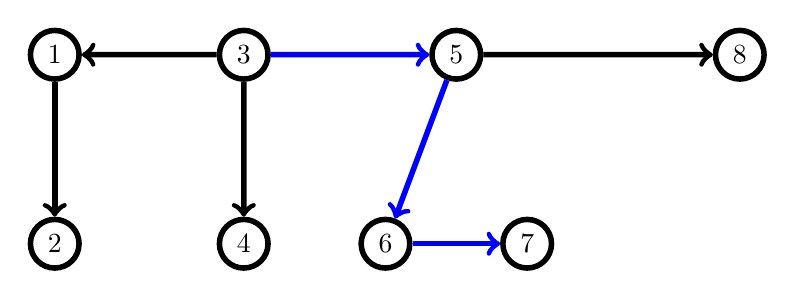
\begin{tikzpicture}[line width=2,scale=1.2]
 \node[circle,draw=black] (1) at (0,2) {$1$};
 \node[circle,draw=black] (2) at (0,0) {$2$};
 \node[circle,draw=black] (3) at (2,2) {$3$};
 \node[circle,draw=black] (4) at (2,0) {$4$};
 \node[circle,draw=black] (5) at (4.25,2) {$5$};
 \node[circle,draw=black] (6) at (3.5,0) {$6$};
 \node[circle,draw=black] (7) at (5,0) {$7$};
 \node[circle,draw=black] (8) at (7.25,2) {$8$};
% \node[circle,draw=black] (9) at (6.5,0) {$9$};
% \node[circle,draw=black] (10) at (8,0) {$10$};
		
 \draw[->] (1) edge (2);
 \draw[->] (3) edge (4);
 \draw[->] (3) edge (1) ;
 \draw[->] (5) edge (8); 
 \draw[->,blue] (3) edge (5) (5) edge (6) (6) edge (7);
\end{tikzpicture}
\end{center} 

Beachten Sie, dass die Knoten $9$ und $10$ nicht im Breitensuchbaum auftreten, da diese vom Startknoten~$s=3$ aus nicht erreichbar sind.
\end{bsp}

\begin{bem} Einige Anwendungen der Breitensuche: 
	\begin{itemize} 
		\item Bestimmen der Zusammenhangskomponente des Knotens $s$ bei einem ungerichteten Graphen $G$. 
		\item Umsetzung von Web-Crawlern, die das Umfeld einer Webseite $s$ bestimmen, das hei\ss t, die Menge von Webseiten, die innerhalb einer vorgegebenen Anzahl $k$ von Klicks von $s$ aus erreichbar sind. 
	\end{itemize}
\end{bem} 

\begin{bem}[Entscheidung von Spielen mit einer Variante der Breitensuche]  		
		Bei verschiedenen Arten von Spielen lässt sich die Frage stellen: Kann man das Gewinnen von einer gegebenen Position aus erzwingen und ggf. wie? Dafür benutzt man etwa im Schach die sogenannten Endspieldatenbanken. 
		Die Generierung von Endspieldatenbanken basiert im Wesentlichen auf der Breitensuche. Vgl. den Abschnitt Generating Tablebases in \url{https://en.wikipedia.org/wiki/Endgame_tablebase}. Endspieldatenbanken kann man für verschiedene Spiele generieren (Treblecross, Hex, Go, Nim usw.), die Anzahl der Positionen ist aber ein mögliches praktisches Hindernis, da der Graph der Endspiele, den man erzeugt, potenziell extrem groß sein kann.   

\condclearpage

		Wir beschreiben eine Art und Weise, die alle Endspiele für eine gegebene Auswahl von Steinen entscheidet: Man erzeugt den Digraphen des Spiels $D=(V,A)$, bei dem jeder Knoten $v \in V$ eine Position (mit gegebener Anzahl der Steine) darstellt, mit dem Vermerk wer dran ist. Die Menge $V$ besteht aus den Knoten, bei denen Weiß dran ist und aus den Knoten, bei denen Schwarz dran ist. Wir zerlegen dementsprechend $V$ als $V = W \cupdot S$. Die Kanten $(a,b) \in A $ stellen die Züge dar, und da Weiß und Schwarz abwechselnd dran sind, gilt für jede Kante entweder  $a \in W,\ b \in S$ oder $a \in S,\ b \in W$. 
		
		Um zu entscheiden, in welchen Stellungen Schwarz den Sieg erzwingen kann, markieren wir die Positionen $a \in W$, bei denen Weiß matt gesetzt ist als \glqq Schwarz gewinnt in $0$\grqq\ Zügen oder kurz $s_0$. Dann markieren wir alle $a \in S$, bei denen $(a,b) \in A$ ist und $b$ als $s_0$ markiert ist als \glqq Schwarz gewinnt in $1$ Zug\grqq\ oder kurz $s_1$. So gehen wir iterativ vor: Sind die Markierungen $s_0,\ldots,s_{k-1}$ bereits vergeben, so bestimmen wir die Knoten $a \in S$, für welche eine Kante $(a,b)$ existiert derart, dass für alle Kanten $(b,c)$, die von $b$ ausgehen, der Knoten $c \in S$ bereits als $s_i$ mit $i=0,\ldots,k-1$ markiert ist. Man markiert $a$ als $s_k$ und merkt sich dabei den Siegeszug $(a,b)$. Auf diese Weise lassen sich alle Positionen markieren, bei denen Schwarz den Sieg erzwingen kann. Analog kann man auch alle Positionen bestimmen, bei denen Weiß den Sieg erzwingen kann.
		Alle nicht markierten Positionen führen beim optimalen Spiel zu unentschieden. 
\end{bem} 

\begin{aufg}\ Nachfolgend eine Illustration des Graphen des Spiels Nim für die Anfangspositionen $(2,2,2)$. Es gibt zwei Startpositionen (für den Fall, dass $A$ beginnt und für den Fall, dass $B$ beginnt). Die Gewinnstrategie für dieses Spiel ist zwar bekannt, man kann den Graphen trotzdem als Illustration zur Lösung der Spiele mit Hilfe von (End)spieldatenbanken benutzen. Berechnen Sie mit Hilfe des Graphen alle Positionen, von denen $A$ (bzw. $B$) den Sieg erzwingen kann. Bei den Positionen, die mit $a$ bzw. $b$ markiert sind, ist $A$ bzw. $B$ dran. Bei Standard-Nim ist die Endposition $b000$ der Sieg für $A$ und $a000$ der Sieg für $B$ (bei Mis\`ere-Nim ist das genau umgekehrt). 
%\begin{center}
%			\includegraphics[width=0.4\textwidth]{Code/nim_222.pdf}
%\end{center}

\begin{center} 
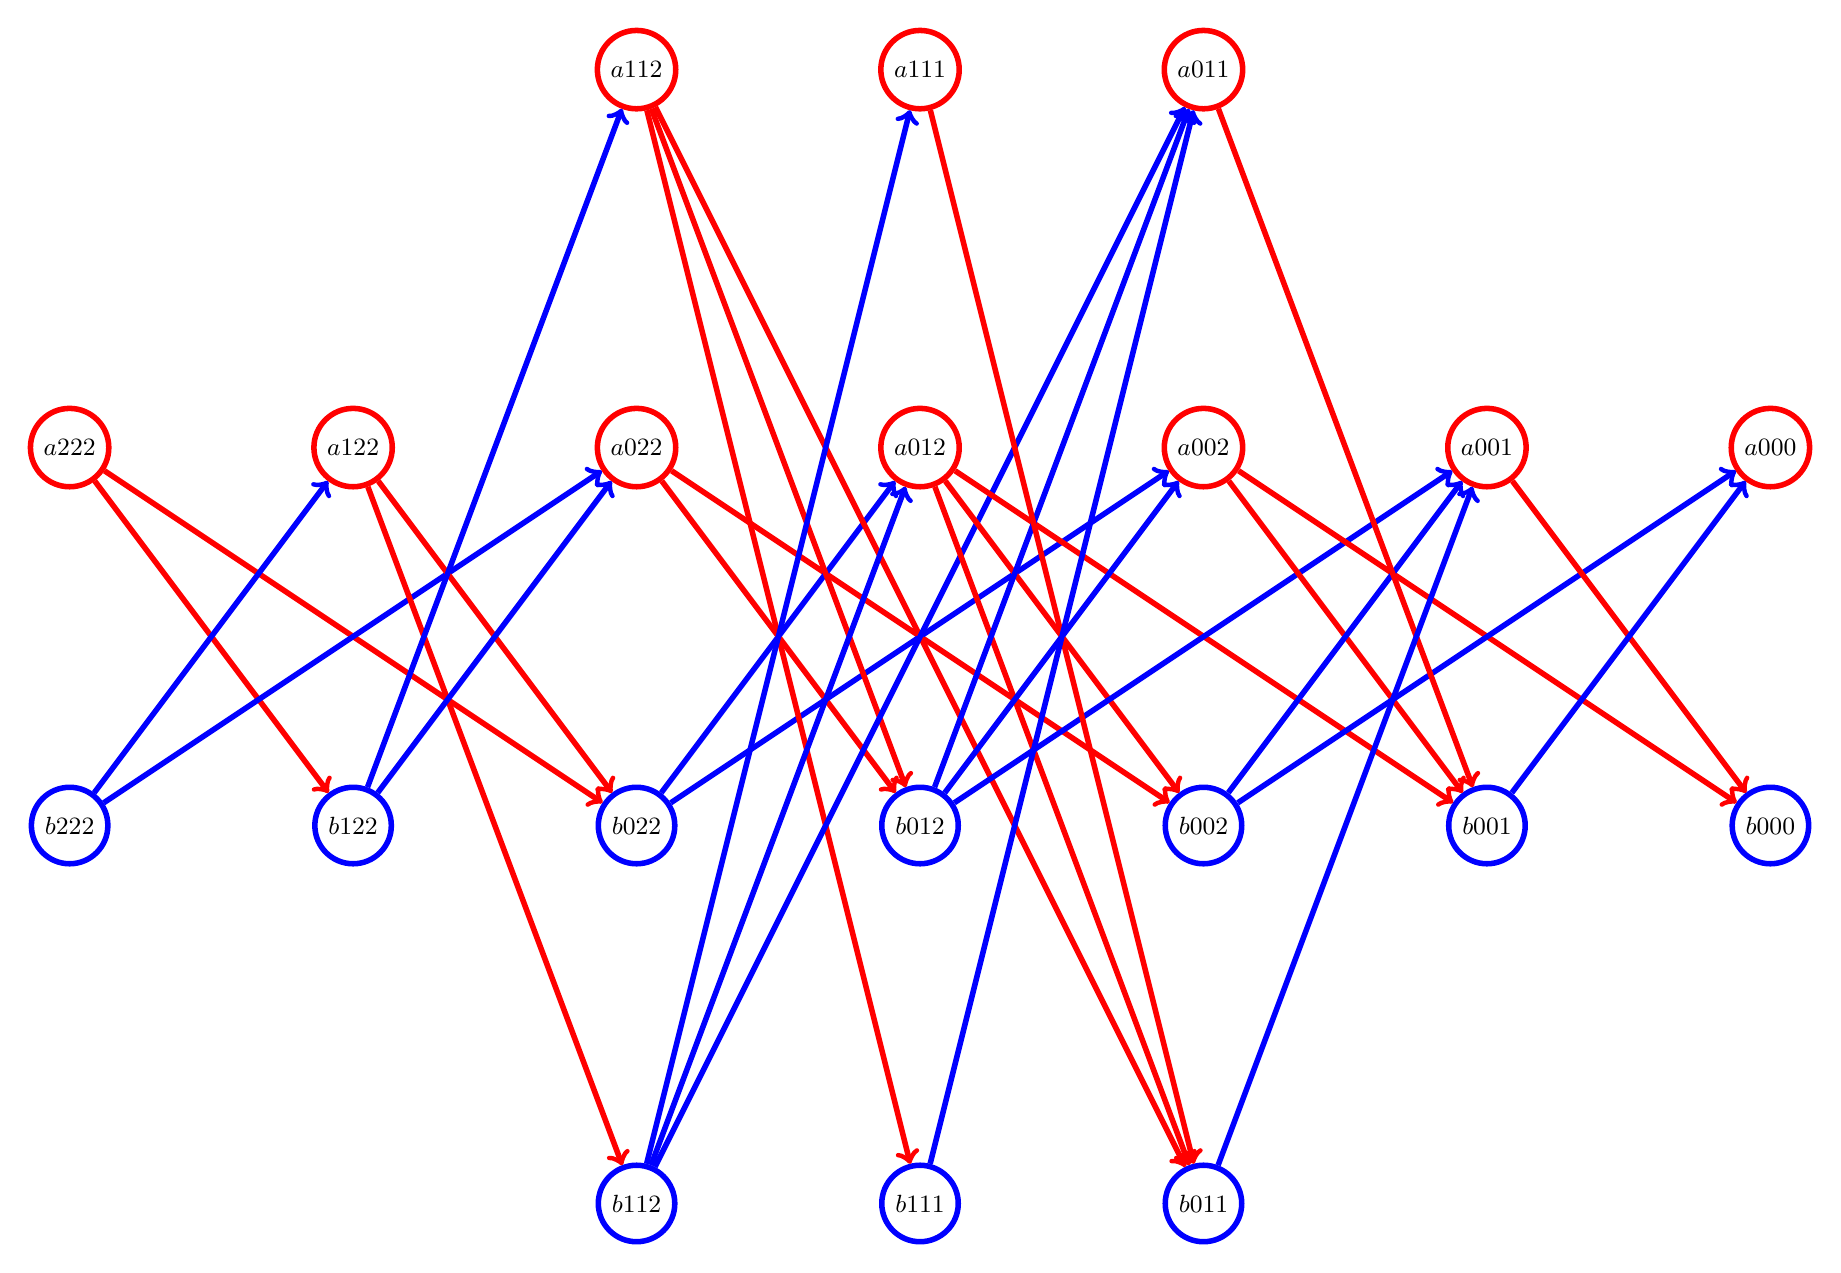
\begin{tikzpicture}[line width=2,scale=1.2]
 \node[circle,draw=red] (a222) at (0,3) {\small $a222$};
 \node[circle,draw=red] (a122) at (3,3) {\small $a122$};
 \node[circle,draw=red] (a022) at (6,3) {\small $a022$};
 \node[circle,draw=red] (a012) at (9,3) {\small $a012$};
 \node[circle,draw=red] (a002) at (12,3) {\small $a002$};
 \node[circle,draw=red] (a001) at (15,3) {\small $a001$};
 \node[circle,draw=red] (a000) at (18,3) {\small $a000$};
 \node[circle,draw=red] (a112) at (6,7) {\small $a112$};
 \node[circle,draw=red] (a111) at (9,7) {\small $a111$};
 \node[circle,draw=red] (a011) at (12,7) {\small $a011$};

 \node[circle,draw=blue] (b222) at (0,-1) {\small $b222$};
 \node[circle,draw=blue] (b122) at (3,-1) {\small $b122$};
 \node[circle,draw=blue] (b022) at (6,-1) {\small $b022$};
 \node[circle,draw=blue] (b012) at (9,-1) {\small $b012$};
 \node[circle,draw=blue] (b002) at (12,-1) {\small $b002$};
 \node[circle,draw=blue] (b001) at (15,-1) {\small $b001$};
 \node[circle,draw=blue] (b000) at (18,-1) {\small $b000$};
 \node[circle,draw=blue] (b112) at (6,-5) {\small $b112$};
 \node[circle,draw=blue] (b111) at (9,-5) {\small $b111$};
 \node[circle,draw=blue] (b011) at (12,-5) {\small $b011$};

 \draw[->,draw=red] (a222) edge (b122);
 \draw[->,draw=red] (a222) edge (b022);
 \draw[->,draw=blue] (b222) edge (a122);
 \draw[->,draw=blue] (b222) edge (a022);

 \draw[->,draw=red] (a122) edge (b112);
 \draw[->,draw=red] (a122) edge (b022);
 \draw[->,draw=blue] (b122) edge (a112);
 \draw[->,draw=blue] (b122) edge (a022);

 \draw[->,draw=red] (a022) edge (b012);
 \draw[->,draw=red] (a022) edge (b002);
 \draw[->,draw=blue] (b022) edge (a012);
 \draw[->,draw=blue] (b022) edge (a002);

 \draw[->,draw=red] (a112) edge (b012);
 \draw[->,draw=red] (a112) edge (b111);
 \draw[->,draw=red] (a112) edge (b011);
 \draw[->,draw=blue] (b112) edge (a012);
 \draw[->,draw=blue] (b112) edge (a111);
 \draw[->,draw=blue] (b112) edge (a011);

 \draw[->,draw=red] (a012) edge (b011);
 \draw[->,draw=red] (a012) edge (b002);
 \draw[->,draw=red] (a012) edge (b001);
 \draw[->,draw=blue] (b012) edge (a011);
 \draw[->,draw=blue] (b012) edge (a002);
 \draw[->,draw=blue] (b012) edge (a001);

 \draw[->,draw=red] (a111) edge (b011);
 \draw[->,draw=blue] (b111) edge (a011);

 \draw[->,draw=red] (a002) edge (b001);
 \draw[->,draw=red] (a002) edge (b000);
 \draw[->,draw=blue] (b002) edge (a001);
 \draw[->,draw=blue] (b002) edge (a000);

 \draw[->,draw=red] (a011) edge (b001);
 \draw[->,draw=blue] (b011) edge (a001);

 \draw[->,draw=red] (a001) edge (b000);
 \draw[->,draw=blue] (b001) edge (a000);
\end{tikzpicture}
\end{center} 
\end{aufg}

\begin{aufg} 
	Wie kann man auf der Basis der Breitensuche testen, ob ein gegebener Graph bipartit ist? 
\end{aufg} 

\begin{aufg}
	Implementieren Sie die Breitensuche. Testen Sie die Laufzeit Ihrer Implementierung auf den realen Straßennetzwerken, die in der 9th DIMACS Implementation Challenge benutzt wurden. Die Graphen sind unter 
	\url{http://www.diag.uniroma1.it/challenge9/download.shtml}  verfügbar. Diese Graphen sind gewichtet: für den Test Ihrer Implementierung können Sie die Gewichte ignorieren. 
\end{aufg} 

\begin{bem}
	Die obige Präsentation der Breitensuche ist in Anlehnung auf \cite{CLRS17} entstanden.
\end{bem} 

\section{Tiefensuche}
\label{sect:tiefensuche}


\begin{bem} 
Die Eingabe für die hier diskutierte Tiefensuche ist ein Digraph $D=(V,A)$.
Ist der Graph ungerichtet, so ist die Vorgehensweise vollkommen analog und daher diskutieren wir hier (fast ausschließlich) die gerichtete Variante.
Der Digraph $D$ ist durch seine Adjazenzliste $N$ gegeben, das heißt, für jeden Knoten $u \in V$ ist $N[u]$ eine Liste aller $v \in V$ mit $(u,v) \in A$.
Die Darstellung von $D$ als Adjazenzliste eine Durchmusterung mit der optimalen Laufzeit $\Theta(|V|+|A|)$ erlaubt.
\end{bem}


\begin{bem} 
	Die Tiefensuche ist ein ``reiselustiger'' Algorithmus zur Durchmusterung von Graphen. Wenn wir Knoten als Orte auffassen und $N[u]$ als die Umgebung des Ortes $u$, so können wir das Grundgerüst der Tiefensuche so beschreiben. Man will alle noch nicht gesehenen Orte erkunden, die man von einem gegebenen Ort $u$ aus erreichen kann. Man kann dazu das folgende Vorgehen benutzen: 
	\begin{itemize} 
			\item Man sucht die Umgebung von $u$ durch. 
			\item Sobald man einen  noch nicht besuchten Ort $v$ sieht, erkundet man alle noch nicht gesehene Orte, die man von $v$ aus erreichen kann. 
	\end{itemize} 
	Der Grundgedanke  der Tiefensuche rekursiv: man erkundet neue Orte von $u$ aus, indem man die Orte erkunden, die man aus noch nicht gesehenen Nachbarschaft von $u$ erreichen kann. Die ``Reiselust'' dieser Durchmusterung besteht darin, dass man sich die Erkundung der Orte \emph{sofort} einen neuen Ort versetzt, wenn ein solcher Ort gefunden wird.  
	
	
	Bei rekursiven Algorithmen soll man sich bei der Umsetzung in der Regel als Erstes darum kümmern, dass der Algorithmus terminiert. Daher soll man bei der Durchmusterung die Orte, an die man kommt, gleich als ``gesehen'' markieren.  Stellen Sie sich einfach vor, dass Sie ein Stück Kreide nehmen und da, wo Sie angekommen sind, gleich schreiben ``hier war ich schon''. Sollten Sie bei Ihrer Wanderung durch den Graphen noch ein mal an diesen Ort kommen,  so werden Sie merken, dass Sie an diesem Ort bereits gewesen sind. Auf diese Weise werden Sie nicht endlos im Kreis herumlaufen, wenn etwa Ihr Graph ein Kreis ist oder einen Kreis enthält. 
	
	Die Umsetzung der oben beschriebenen Strategie basiert auf Farbattributen der Knoten, die man im Laufe der Durchmusterung sukzessiv zuerst als weiß ($=$ noch nicht gesehen), dann als  grau ($=$ gesehen aber noch nicht abgearbeitet) und schließlich als  schwarz ($=$ abgearbeitet) setzt. 
\end{bem}

\begin{defn}
	Wenn die Tiefensuche entlang einer Kante verläuft, die in einen weißen Knoten endet, dann sagen wir, dass der entsprechende Knoten \textbf{entdeckt} wird.

Hier eine Zusammenfassung der Bedeutung der Farben der Knoten.  
\begin{itemize}
	\item[] {\bfseries weiß:} Der Knoten wurde noch nicht entdeckt. 
	\item[] {\bfseries grau:} Der Knoten wurde entdeckt und die Tiefensuche für den Knoten läuft gerade.
	\item[] {\bfseries schwarz:} Der Knoten wurde entdeckt und die Tiefensuche für den Knoten ist bereits beendet.
\end{itemize}

Wird ein Knoten schwarz gefärbt, so sagen wir auch das er \textbf{abgearbeitet} wurde.

Durch die Tiefensuche können verschiedene Aufgaben erledigt werden. Nicht alle diese Aufgaben benötigen alle drei Farbattributen der Knoten. Bei manchen Aufgaben reicht auch die Unterscheidung zwischen ``entdeckt'' (weiß) und ``nicht entdeckt'' (grau oder schwarz) aus. 
\end{defn}

\begin{bem}
	Auf diese Weise können wir die Tiefensuche initialisiert: 
	\begin{algorithm} 
		\caption{$\cc{Tiefensuche-Initialisieren}(D)$}
	\begin{algorithmic}[1]
		\FOR{$u \in V$}
		\STATE $\cc{Farbe}[u]=\cc{weiß}$
		\STATE $\pi[u]=\cc{nil}$
		\ENDFOR
		\end{algorithmic}
	\end{algorithm} 
\end{bem}  


\begin{bem} Sobald die Initialisierung erfolgt ist, können wir die Tiefensuche von einem gegebenen Knoten ausführen. Hier die rekursive Umsetzung: 
	\begin{algorithm}[H]
		\caption{$\cc{Tiefensuche}(u)$}
		\begin{algorithmic}[1]
			\STATE $\cc{Farbe}[u]:=\cc{grau}$ \ \COMMENT{$u$ als entdeckt notiert} 
			\FOR{$v \in N[u]$}
			\STATE  \COMMENT{Die Kante $(u,v)$ wird sondiert}
			\IF{$\cc{Farbe}[v]=\cc{weiß}$}
			\STATE $\pi[v]:=u$   \ \COMMENT{Knoten $v$ wurde entdeckt} 
			\STATE $\cc{Tiefensuche}(v)$
			\ENDIF
			\ENDFOR
			\STATE $\cc{Farbe}[u]:=\cc{schwarz}$ 
		\end{algorithmic}
	\end{algorithm}
\end{bem}

\begin{bem} 
	Die Prozedur Tiefensuche können wir in den folgenden Rahmen einbauen. 
	\begin{algorithm}[H]
		\caption{$\cc{Vollständige-Tiefensuche}(D)$}
		\begin{algorithmic}[1]
			\STATE $\cc{Tiefensuche-Initialisieiren}(D)$ 
			\FOR{$u \in V$}\label{line:tiefensuche-hauptschleife-start}
			\IF{$\cc{Farbe}[u]=\cc{weiß}$}
			\STATE $\cc{Tiefensuche}(u)$
			\ENDIF 
			\ENDFOR\label{line:tiefensuche-hauptschleife-ende}
		\end{algorithmic}
	\end{algorithm}
	Durch diese Prozedur entdecken wir jeden jeden Knoten genau ein mal und sondieren dabei jede Kante von $D=(V,A)$. 
\end{bem}




\begin{bem}[Variante mit Zeitstempeln] 
 Jeder Knoten $v \in V$ kann während der Tiefensuche mit zwei \emph{Zeitstempeln} versehen werden: Der erste Zeitstempel $\cc{Grau}[v]$ zeichnet auf, wann der Knoten grau gefärbt wird, das heißt, wann er das erste Mal entdeckt wird.
Der zweite Zeitstempel $\cc{Schwarz}[v]$ hingegen, speichert den Zeitpunkt der Schwarzfärbung von~$v$, das heißt, den Moment in dem der Knoten abgearbeitet ist.

Im Algorithmus werden beide Zeitstempel ganze Zahlen zwischen $1$ und $2 |V|$ sein, da es für jeden Knoten $v \in V$ genau einen Zeitpunkt der Entdeckung (Graufärbung) und einen Zeitpunkt der Abarbeitung (Schwarzfärbung) gibt.

Für jedes $v \in V$ gilt $\cc{Grau}[v] < \cc{Schwarz}[v]$.
Weiterhin ist $v$ vor dem Zeitpunkt $\cc{Grau}[v]$ weiß, während der Zeitpunkte $\cc{Grau}[v],\ldots,\cc{Schwarz}[v]-1$ grau, und ab dem Zeitpunkt $\cc{Schwarz}[v]$ schwarz.

Für die Variante mit den Zeitstempeln sollen die Initialisierung und die Tiefensuche geringfügig ergänzt werden. 

Die Initialisierung: 

	\begin{algorithm} 
	\caption{$\cc{Tiefensuche-Initialisieren}(D)$}
	\begin{algorithmic}[1]
		\FOR{$u \in V$}
		\STATE $\cc{Farbe}[u]=\cc{weiß}$
		\STATE $\pi[u]=\cc{nil}$
		\ENDFOR
		\STATE {\color{red} $t:=0$ \quad \COMMENT{Initialisierung der Zeit-Variablen} }
	\end{algorithmic}
\end{algorithm} 

Die Tiefensuche: 

\begin{algorithm}[H]
	\caption{$\cc{Tiefensuche}(u)$}
	\begin{algorithmic}[1]
		\STATE {\color{red} $t := t + 1$ $\quad$ \COMMENT{Die Uhr tickt vor jeder Färbung} }
		\STATE { \color{red} $\cc{Grau}[u] := t$ $\quad$ \COMMENT{Der Knoten $u$ wurde gerade entdeckt} }
		\STATE $\cc{Farbe}[u]:=\cc{grau}$
		\FOR{$v \in N[u]$}
		\IF{$\cc{Farbe}[v]=\cc{weiß}$}
		 \STATE $\pi[v]:=u$  
		\STATE $\cc{Tiefensuche}(v)$
		\ENDIF
		\ENDFOR
		\STATE {\color{red} $t := t + 1$ $\quad$ \COMMENT{Die Uhr tickt vor jeder Färbung} }
		\STATE\label{line:schwarzfaerbung-in-tiefensuche} {\color{red} $\cc{Schwarz}[u] := t$ $\quad$ \COMMENT{Der Knoten $u$ wurde gerade abgearbeitet}}
		\STATE $\cc{Farbe}[u]:=\cc{schwarz}$
	\end{algorithmic}
\end{algorithm}
\end{bem}

\begin{bsp}
\label{bsp:tiefensuche}
Wir illustrieren die Tiefensuche am Digraphen

\hfill
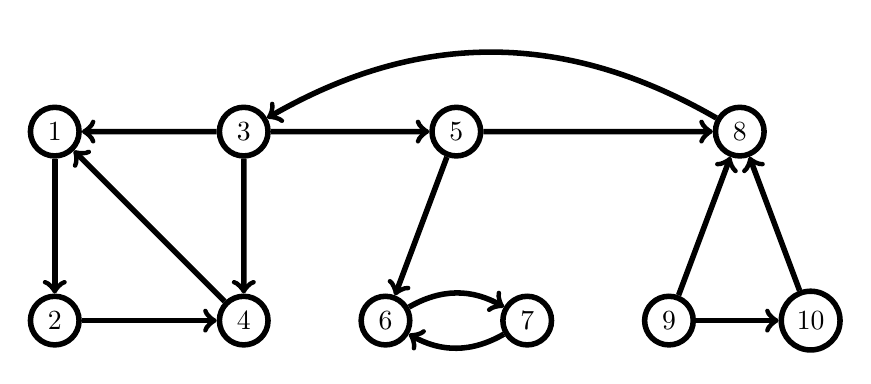
\begin{tikzpicture}[line width=2,scale=1.2]
 \node[circle,draw=black] (1) at (0,2) {$1$};
 \node[circle,draw=black] (2) at (0,0) {$2$};
 \node[circle,draw=black] (3) at (2,2) {$3$};
 \node[circle,draw=black] (4) at (2,0) {$4$};
 \node[circle,draw=black] (5) at (4.25,2) {$5$};
 \node[circle,draw=black] (6) at (3.5,0) {$6$};
 \node[circle,draw=black] (7) at (5,0) {$7$};
 \node[circle,draw=black] (8) at (7.25,2) {$8$};
 \node[circle,draw=black] (9) at (6.5,0) {$9$};
 \node[circle,draw=black] (10) at (8,0) {$10$};
		
 \draw[->] (1) edge (2);
 \draw[->] (2) edge (4);
 \draw[->] (3) edge (1) (3) edge (4) (3) edge (5);
 \draw[->] (4) edge (1);
 \draw[->] (5) edge (6) (5) edge (8); 
 \draw[->] (6) to[bend left] (7);
 \draw[->] (7) to[bend left] (6);
 \draw[->] (8) to[bend right] (3);
 \draw[->] (9) edge (8) (9) edge (10);
 \draw[->] (10) edge (8); 
\end{tikzpicture}
\hfill\,

Wir wählen als Startknoten den Knoten~$3$ und treffen ansonsten jede Wahl aufsteigend in der Reihenfolge der Knotenindizes.
Die ersten sechs Zeitschritte sind durch die folgende Sequenz von gefärbten Digraphen gegeben, wobei die Knotenfarbe dem aktuellen Farbattribut entspricht und die bereits sondierten Kanten rot markiert sind:

\condclearpage 

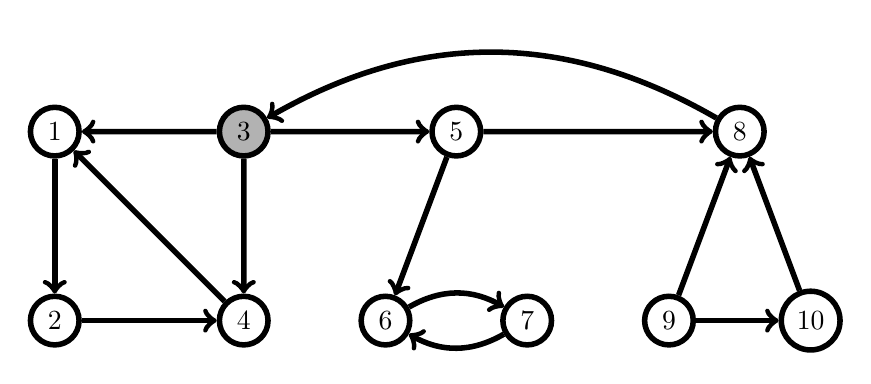
\begin{tikzpicture}[line width=2,scale=1.2]
 \tikzset{gnode/.style ={fill=black!30!,circle,draw}}
 \tikzset{snode/.style ={white,fill=black,circle,draw}}

 \node[circle,draw=black] (1) at (0,2) {$1$};
 \node[circle,draw=black] (2) at (0,0) {$2$};
 \node[gnode] (3) at (2,2) {$3$};
 \node[circle,draw=black] (4) at (2,0) {$4$};
 \node[circle,draw=black] (5) at (4.25,2) {$5$};
 \node[circle,draw=black] (6) at (3.5,0) {$6$};
 \node[circle,draw=black] (7) at (5,0) {$7$};
 \node[circle,draw=black] (8) at (7.25,2) {$8$};
 \node[circle,draw=black] (9) at (6.5,0) {$9$};
 \node[circle,draw=black] (10) at (8,0) {$10$};
		
 \draw[->] (1) edge (2);
 \draw[->] (2) edge (4);
 \draw[->] (3) edge (1) (3) edge (4) (3) edge (5);
 \draw[->] (4) edge (1);
 \draw[->] (5) edge (6) (5) edge (8); 
 \draw[->] (6) to[bend left] (7);
 \draw[->] (7) to[bend left] (6);
 \draw[->] (8) to[bend right] (3);
 \draw[->] (9) edge (8) (9) edge (10);
 \draw[->] (10) edge (8); 
\end{tikzpicture}
\\ $TS(3)$ 

\condclearpage 

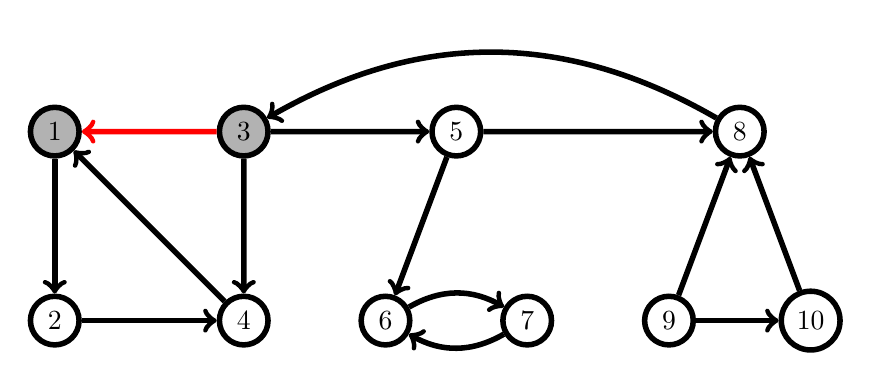
\begin{tikzpicture}[line width=2,scale=1.2]
 \tikzset{gnode/.style ={fill=black!30!,circle,draw}}
 \tikzset{snode/.style ={white,fill=black,circle,draw}}

 \node[gnode] (1) at (0,2) {$1$};
 \node[circle,draw=black] (2) at (0,0) {$2$};
 \node[gnode] (3) at (2,2) {$3$};
 \node[circle,draw=black] (4) at (2,0) {$4$};
 \node[circle,draw=black] (5) at (4.25,2) {$5$};
 \node[circle,draw=black] (6) at (3.5,0) {$6$};
 \node[circle,draw=black] (7) at (5,0) {$7$};
 \node[circle,draw=black] (8) at (7.25,2) {$8$};
 \node[circle,draw=black] (9) at (6.5,0) {$9$};
 \node[circle,draw=black] (10) at (8,0) {$10$};
		
 \draw[->] (1) edge (2);
 \draw[->] (2) edge (4);
 \draw[->,red] (3) edge (1);
 \draw[->] (3) edge (4) (3) edge (5);
 \draw[->] (4) edge (1);
 \draw[->] (5) edge (6) (5) edge (8); 
 \draw[->] (6) to[bend left] (7);
 \draw[->] (7) to[bend left] (6);
 \draw[->] (8) to[bend right] (3);
 \draw[->] (9) edge (8) (9) edge (10);
 \draw[->] (10) edge (8); 
\end{tikzpicture}
\\ $TS(3) \to TS(1)$ 

\condclearpage 
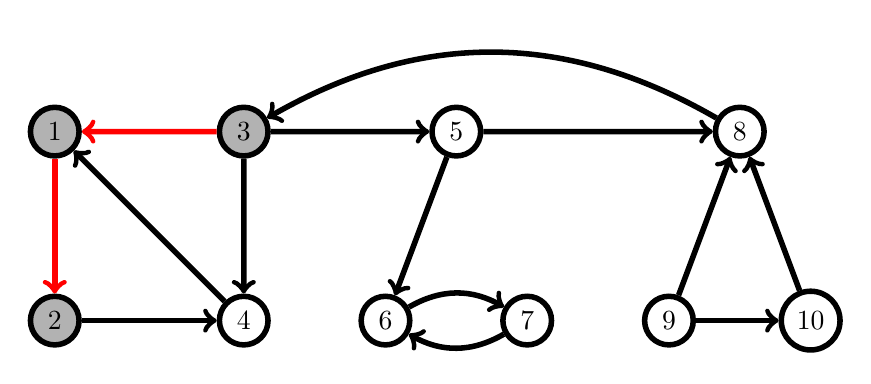
\begin{tikzpicture}[line width=2,scale=1.2]
 \tikzset{gnode/.style ={fill=black!30!,circle,draw}}
 \tikzset{snode/.style ={white,fill=black,circle,draw}}

 \node[gnode] (1) at (0,2) {$1$};
 \node[gnode] (2) at (0,0) {$2$};
 \node[gnode] (3) at (2,2) {$3$};
 \node[circle,draw=black] (4) at (2,0) {$4$};
 \node[circle,draw=black] (5) at (4.25,2) {$5$};
 \node[circle,draw=black] (6) at (3.5,0) {$6$};
 \node[circle,draw=black] (7) at (5,0) {$7$};
 \node[circle,draw=black] (8) at (7.25,2) {$8$};
 \node[circle,draw=black] (9) at (6.5,0) {$9$};
 \node[circle,draw=black] (10) at (8,0) {$10$};
		
 \draw[->,red] (1) edge (2);
 \draw[->] (2) edge (4);
 \draw[->,red] (3) edge (1);
 \draw[->] (3) edge (4) (3) edge (5);
 \draw[->] (4) edge (1);
 \draw[->] (5) edge (6) (5) edge (8); 
 \draw[->] (6) to[bend left] (7);
 \draw[->] (7) to[bend left] (6);
 \draw[->] (8) to[bend right] (3);
 \draw[->] (9) edge (8) (9) edge (10);
 \draw[->] (10) edge (8); 
\end{tikzpicture}
\\ $TS(3)\to TS(1) \to TS(2)$  

\condclearpage 
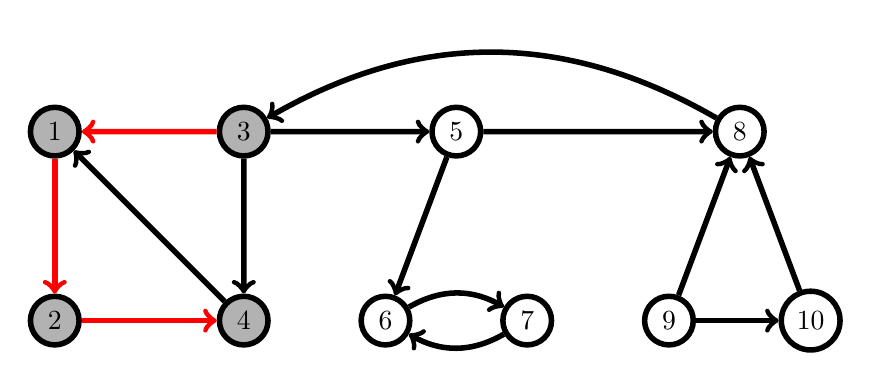
\begin{tikzpicture}[line width=2,scale=1.2]
 \tikzset{gnode/.style ={fill=black!30!,circle,draw}}
 \tikzset{snode/.style ={white,fill=black,circle,draw}}

 \node[gnode] (1) at (0,2) {$1$};
 \node[gnode] (2) at (0,0) {$2$};
 \node[gnode] (3) at (2,2) {$3$};
 \node[gnode] (4) at (2,0) {$4$};
 \node[circle,draw=black] (5) at (4.25,2) {$5$};
 \node[circle,draw=black] (6) at (3.5,0) {$6$};
 \node[circle,draw=black] (7) at (5,0) {$7$};
 \node[circle,draw=black] (8) at (7.25,2) {$8$};
 \node[circle,draw=black] (9) at (6.5,0) {$9$};
 \node[circle,draw=black] (10) at (8,0) {$10$};
		
 \draw[->,red] (1) edge (2);
 \draw[->,red] (2) edge (4);
 \draw[->,red] (3) edge (1);
 \draw[->] (3) edge (4) (3) edge (5);
 \draw[->] (4) edge (1);
 \draw[->] (5) edge (6) (5) edge (8); 
 \draw[->] (6) to[bend left] (7);
 \draw[->] (7) to[bend left] (6);
 \draw[->] (8) to[bend right] (3);
 \draw[->] (9) edge (8) (9) edge (10);
 \draw[->] (10) edge (8); 
\end{tikzpicture}
\\ $TS(3)\to TS(1) \to TS(2) \to TS(4)$ 

\condclearpage
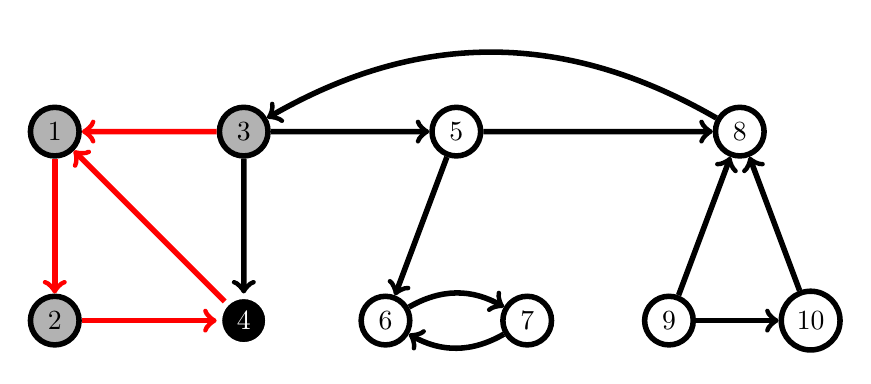
\begin{tikzpicture}[line width=2,scale=1.2]
 \tikzset{gnode/.style ={fill=black!30!,circle,draw}}
\tikzset{snode/.style ={white,fill=black,circle,draw}}

 \node[gnode] (1) at (0,2) {$1$};
 \node[gnode] (2) at (0,0) {$2$};
 \node[gnode] (3) at (2,2) {$3$};
 \node[snode] (4) at (2,0) {$4$};
 \node[circle,draw=black] (5) at (4.25,2) {$5$};
 \node[circle,draw=black] (6) at (3.5,0) {$6$};
 \node[circle,draw=black] (7) at (5,0) {$7$};
 \node[circle,draw=black] (8) at (7.25,2) {$8$};
 \node[circle,draw=black] (9) at (6.5,0) {$9$};
 \node[circle,draw=black] (10) at (8,0) {$10$};
		
 \draw[->,red] (1) edge (2);
 \draw[->,red] (2) edge (4);
 \draw[->,red] (3) edge (1);
 \draw[->] (3) edge (4) (3) edge (5);
 \draw[->,red] (4) edge (1);
 \draw[->] (5) edge (6) (5) edge (8); 
 \draw[->] (6) to[bend left] (7);
 \draw[->] (7) to[bend left] (6);
 \draw[->] (8) to[bend right] (3);
 \draw[->] (9) edge (8) (9) edge (10);
 \draw[->] (10) edge (8); 
\end{tikzpicture}
\\ $TS(3)\to TS(1) \to TS(2)$

\condclearpage 
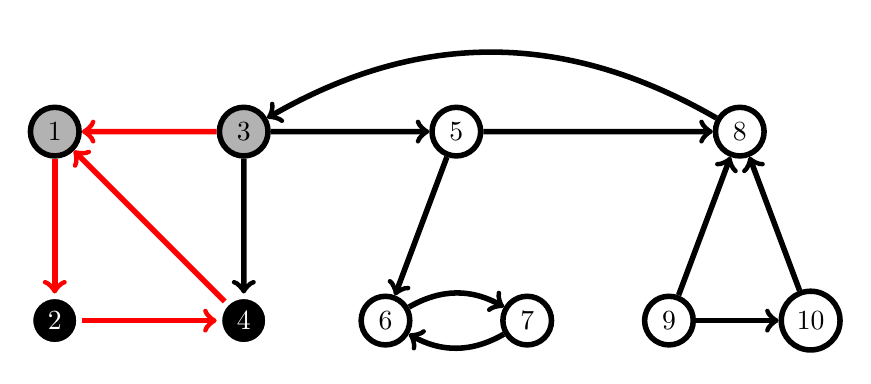
\begin{tikzpicture}[line width=2,scale=1.2]
 \tikzset{gnode/.style ={fill=black!30!,circle,draw}}
 \tikzset{snode/.style ={white,fill=black,circle,draw}}

 \node[gnode] (1) at (0,2) {$1$};
 \node[snode] (2) at (0,0) {$2$};
 \node[gnode] (3) at (2,2) {$3$};
 \node[snode] (4) at (2,0) {$4$};
 \node[circle,draw=black] (5) at (4.25,2) {$5$};
 \node[circle,draw=black] (6) at (3.5,0) {$6$};
 \node[circle,draw=black] (7) at (5,0) {$7$};
 \node[circle,draw=black] (8) at (7.25,2) {$8$};
 \node[circle,draw=black] (9) at (6.5,0) {$9$};
 \node[circle,draw=black] (10) at (8,0) {$10$};
		
 \draw[->,red] (1) edge (2);
 \draw[->,red] (2) edge (4);
 \draw[->,red] (3) edge (1);
 \draw[->] (3) edge (4) (3) edge (5);
 \draw[->,red] (4) edge (1);
 \draw[->] (5) edge (6) (5) edge (8); 
 \draw[->] (6) to[bend left] (7);
 \draw[->] (7) to[bend left] (6);
 \draw[->] (8) to[bend right] (3);
 \draw[->] (9) edge (8) (9) edge (10);
 \draw[->] (10) edge (8); 
\end{tikzpicture}
\\ $TS(3)\to TS(1)$

Wir steigen zum Zeitpunkt $\cc{Schwarz}[8]=14$ mit der Illustration wieder ein:

\condclearpage 
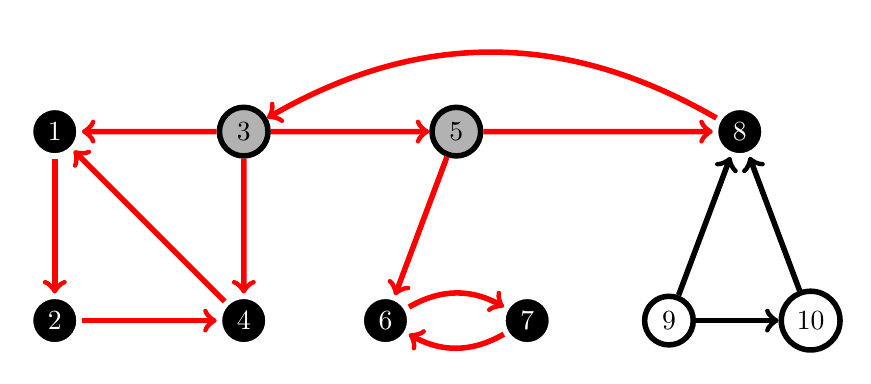
\begin{tikzpicture}[line width=2,scale=1.2]
 \tikzset{gnode/.style ={fill=black!30!,circle,draw}}
 \tikzset{snode/.style ={white,fill=black,circle,draw}}

 \node[snode] (1) at (0,2) {$1$};
 \node[snode] (2) at (0,0) {$2$};
 \node[gnode] (3) at (2,2) {$3$};
 \node[snode] (4) at (2,0) {$4$};
 \node[gnode] (5) at (4.25,2) {$5$};
 \node[snode] (6) at (3.5,0) {$6$};
 \node[snode] (7) at (5,0) {$7$};
 \node[snode] (8) at (7.25,2) {$8$};
 \node[circle,draw=black] (9) at (6.5,0) {$9$};
 \node[circle,draw=black] (10) at (8,0) {$10$};
		
 \draw[->,red] (1) edge (2);
 \draw[->,red] (2) edge (4);
 \draw[->,red] (3) edge (1);
 \draw[->,red] (3) edge (4) (3) edge (5);
 \draw[->,red] (4) edge (1);
 \draw[->,red] (5) edge (6) (5) edge (8); 
 \draw[->,red] (6) to[bend left] (7);
 \draw[->,red] (7) to[bend left] (6);
 \draw[->,red] (8) to[bend right] (3);
 \draw[->] (9) edge (8) (9) edge (10);
 \draw[->] (10) edge (8); 
\end{tikzpicture}
\\ $TS(3)\to TS(5)$

\condclearpage 
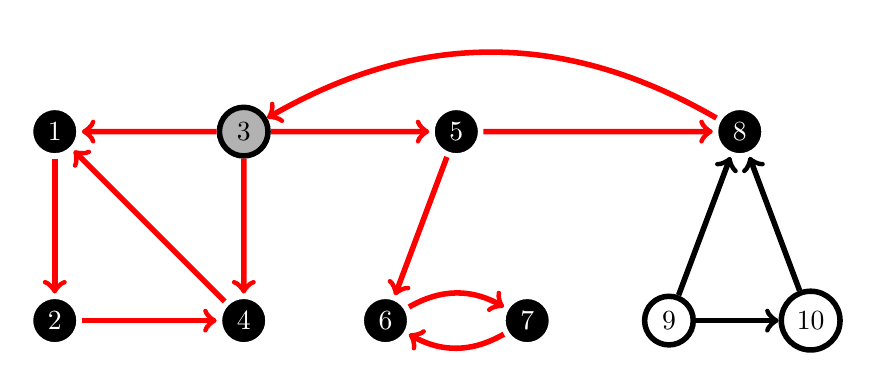
\begin{tikzpicture}[line width=2,scale=1.2]
 \tikzset{gnode/.style ={fill=black!30!,circle,draw}}
 \tikzset{snode/.style ={white,fill=black,circle,draw}}

 \node[snode] (1) at (0,2) {$1$};
 \node[snode] (2) at (0,0) {$2$};
 \node[gnode] (3) at (2,2) {$3$};
 \node[snode] (4) at (2,0) {$4$};
 \node[snode] (5) at (4.25,2) {$5$};
 \node[snode] (6) at (3.5,0) {$6$};
 \node[snode] (7) at (5,0) {$7$};
 \node[snode] (8) at (7.25,2) {$8$};
 \node[circle,draw=black] (9) at (6.5,0) {$9$};
 \node[circle,draw=black] (10) at (8,0) {$10$};
		
 \draw[->,red] (1) edge (2);
 \draw[->,red] (2) edge (4);
 \draw[->,red] (3) edge (1);
 \draw[->,red] (3) edge (4) (3) edge (5);
 \draw[->,red] (4) edge (1);
 \draw[->,red] (5) edge (6) (5) edge (8); 
 \draw[->,red] (6) to[bend left] (7);
 \draw[->,red] (7) to[bend left] (6);
 \draw[->,red] (8) to[bend right] (3);
 \draw[->] (9) edge (8) (9) edge (10);
 \draw[->] (10) edge (8); 
\end{tikzpicture}
\hfill\,

\condclearpage 
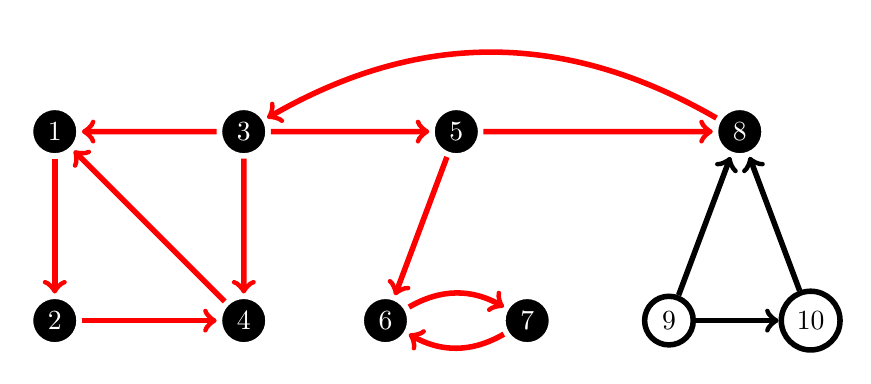
\begin{tikzpicture}[line width=2,scale=1.2]
 \tikzset{gnode/.style ={fill=black!30!,circle,draw}}
 \tikzset{snode/.style ={white,fill=black,circle,draw}}

 \node[snode] (1) at (0,2) {$1$};
 \node[snode] (2) at (0,0) {$2$};
 \node[snode] (3) at (2,2) {$3$};
 \node[snode] (4) at (2,0) {$4$};
 \node[snode] (5) at (4.25,2) {$5$};
 \node[snode] (6) at (3.5,0) {$6$};
 \node[snode] (7) at (5,0) {$7$};
 \node[snode] (8) at (7.25,2) {$8$};
 \node[circle,draw=black] (9) at (6.5,0) {$9$};
 \node[circle,draw=black] (10) at (8,0) {$10$};
		
 \draw[->,red] (1) edge (2);
 \draw[->,red] (2) edge (4);
 \draw[->,red] (3) edge (1);
 \draw[->,red] (3) edge (4) (3) edge (5);
 \draw[->,red] (4) edge (1);
 \draw[->,red] (5) edge (6) (5) edge (8); 
 \draw[->,red] (6) to[bend left] (7);
 \draw[->,red] (7) to[bend left] (6);
 \draw[->,red] (8) to[bend right] (3);
 \draw[->] (9) edge (8) (9) edge (10);
 \draw[->] (10) edge (8); 
\end{tikzpicture}
\hfill\,

Nun muss ein neuer Knoten gewählt werden (Knoten $9$) um die Tiefensuche für den ganzen Digraphen zu beenden:

\condclearpage 
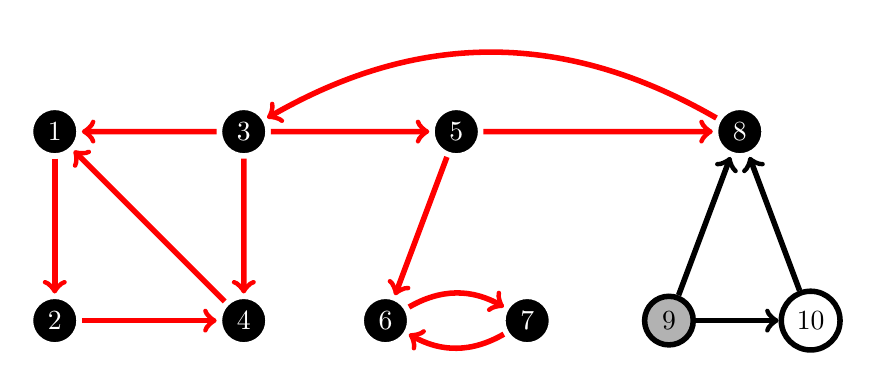
\begin{tikzpicture}[line width=2,scale=1.2]
 \tikzset{gnode/.style ={fill=black!30!,circle,draw}}
 \tikzset{snode/.style ={white,fill=black,circle,draw}}

 \node[snode] (1) at (0,2) {$1$};
 \node[snode] (2) at (0,0) {$2$};
 \node[snode] (3) at (2,2) {$3$};
 \node[snode] (4) at (2,0) {$4$};
 \node[snode] (5) at (4.25,2) {$5$};
 \node[snode] (6) at (3.5,0) {$6$};
 \node[snode] (7) at (5,0) {$7$};
 \node[snode] (8) at (7.25,2) {$8$};
 \node[gnode] (9) at (6.5,0) {$9$};
 \node[circle,draw=black] (10) at (8,0) {$10$};
		
 \draw[->,red] (1) edge (2);
 \draw[->,red] (2) edge (4);
 \draw[->,red] (3) edge (1);
 \draw[->,red] (3) edge (4) (3) edge (5);
 \draw[->,red] (4) edge (1);
 \draw[->,red] (5) edge (6) (5) edge (8); 
 \draw[->,red] (6) to[bend left] (7);
 \draw[->,red] (7) to[bend left] (6);
 \draw[->,red] (8) to[bend right] (3);
 \draw[->] (9) edge (8) (9) edge (10);
 \draw[->] (10) edge (8); 
\end{tikzpicture}
\hfill\,

\condclearpage 
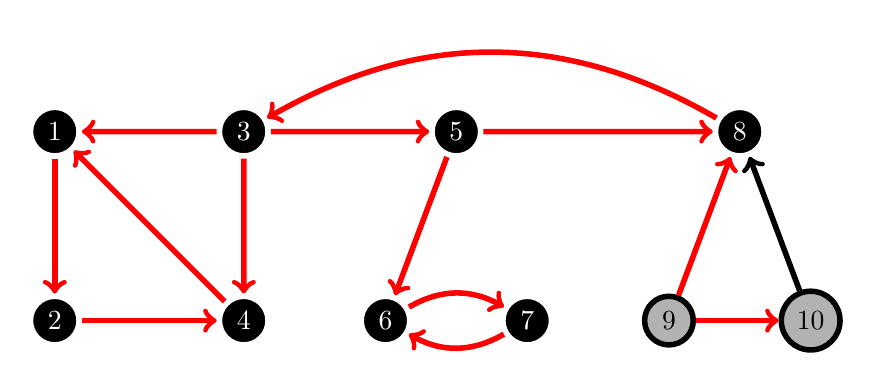
\begin{tikzpicture}[line width=2,scale=1.2]
 \tikzset{gnode/.style ={fill=black!30!,circle,draw}}
 \tikzset{snode/.style ={white,fill=black,circle,draw}}

 \node[snode] (1) at (0,2) {$1$};
 \node[snode] (2) at (0,0) {$2$};
 \node[snode] (3) at (2,2) {$3$};
 \node[snode] (4) at (2,0) {$4$};
 \node[snode] (5) at (4.25,2) {$5$};
 \node[snode] (6) at (3.5,0) {$6$};
 \node[snode] (7) at (5,0) {$7$};
 \node[snode] (8) at (7.25,2) {$8$};
 \node[gnode] (9) at (6.5,0) {$9$};
 \node[gnode] (10) at (8,0) {$10$};
		
 \draw[->,red] (1) edge (2);
 \draw[->,red] (2) edge (4);
 \draw[->,red] (3) edge (1);
 \draw[->,red] (3) edge (4) (3) edge (5);
 \draw[->,red] (4) edge (1);
 \draw[->,red] (5) edge (6) (5) edge (8); 
 \draw[->,red] (6) to[bend left] (7);
 \draw[->,red] (7) to[bend left] (6);
 \draw[->,red] (8) to[bend right] (3);
 \draw[->,red] (9) edge (8) (9) edge (10);
 \draw[->] (10) edge (8); 
\end{tikzpicture}
\hfill\,

\condclearpage 
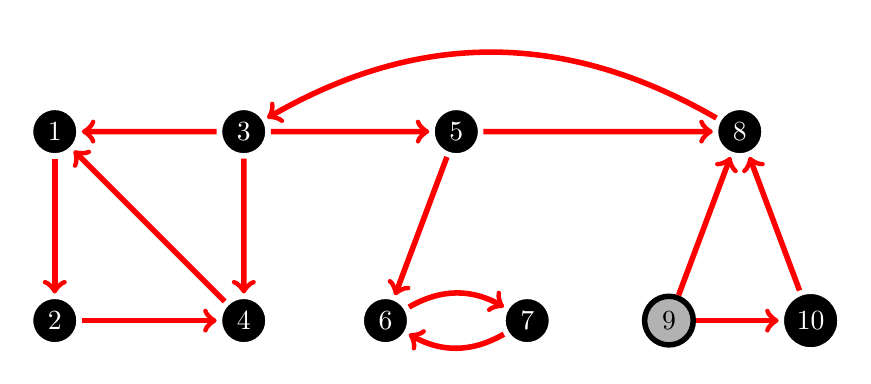
\begin{tikzpicture}[line width=2,scale=1.2]
 \tikzset{gnode/.style ={fill=black!30!,circle,draw}}
 \tikzset{snode/.style ={white,fill=black,circle,draw}}

 \node[snode] (1) at (0,2) {$1$};
 \node[snode] (2) at (0,0) {$2$};
 \node[snode] (3) at (2,2) {$3$};
 \node[snode] (4) at (2,0) {$4$};
 \node[snode] (5) at (4.25,2) {$5$};
 \node[snode] (6) at (3.5,0) {$6$};
 \node[snode] (7) at (5,0) {$7$};
 \node[snode] (8) at (7.25,2) {$8$};
 \node[gnode] (9) at (6.5,0) {$9$};
 \node[snode] (10) at (8,0) {$10$};
		
 \draw[->,red] (1) edge (2);
 \draw[->,red] (2) edge (4);
 \draw[->,red] (3) edge (1);
 \draw[->,red] (3) edge (4) (3) edge (5);
 \draw[->,red] (4) edge (1);
 \draw[->,red] (5) edge (6) (5) edge (8); 
 \draw[->,red] (6) to[bend left] (7);
 \draw[->,red] (7) to[bend left] (6);
 \draw[->,red] (8) to[bend right] (3);
 \draw[->,red] (9) edge (8) (9) edge (10);
 \draw[->,red] (10) edge (8); 
\end{tikzpicture}
\hfill\,

\condclearpage 
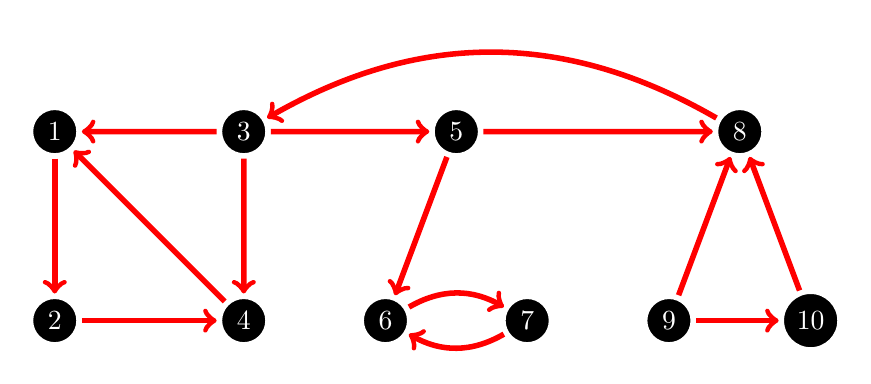
\begin{tikzpicture}[line width=2,scale=1.2]
 \tikzset{gnode/.style ={fill=black!30!,circle,draw}}
 \tikzset{snode/.style ={white,fill=black,circle,draw}}

 \node[snode] (1) at (0,2) {$1$};
 \node[snode] (2) at (0,0) {$2$};
 \node[snode] (3) at (2,2) {$3$};
 \node[snode] (4) at (2,0) {$4$};
 \node[snode] (5) at (4.25,2) {$5$};
 \node[snode] (6) at (3.5,0) {$6$};
 \node[snode] (7) at (5,0) {$7$};
 \node[snode] (8) at (7.25,2) {$8$};
 \node[snode] (9) at (6.5,0) {$9$};
 \node[snode] (10) at (8,0) {$10$};
		
 \draw[->,red] (1) edge (2);
 \draw[->,red] (2) edge (4);
 \draw[->,red] (3) edge (1);
 \draw[->,red] (3) edge (4) (3) edge (5);
 \draw[->,red] (4) edge (1);
 \draw[->,red] (5) edge (6) (5) edge (8); 
 \draw[->,red] (6) to[bend left] (7);
 \draw[->,red] (7) to[bend left] (6);
 \draw[->,red] (8) to[bend right] (3);
 \draw[->,red] (9) edge (8) (9) edge (10);
 \draw[->,red] (10) edge (8); 
\end{tikzpicture}
\hfill\,

Nun sind alle Knoten schwarz und die Tiefensuche ist beendet.
\end{bsp}

%Als Beispiel kann man die TS mit dem Startknoten $1$ im Fall von $N$:
%\[
%	\begin{array}{llll}
%	1: & 2, & 4 
%	\\ 2: & 3
%	\\ 3: & 
%	\\ 4: & 2, & 3, & 5
%	\\ 5: & 6
%	\\ 6: & 4
%	\\ 7: & 6
%	\end{array}
%\]
%betrachten. Wir protokollieren die Änderungen wann welche TSen aufgerufen und beendet werden und wie sich die Farben der Knoten ändern. *****

\begin{bem}
	Bevor wir die Anwendungen der Tiefensuche diskutieren, analysieren wir Ihre Laufzeit. 
\end{bem} 

\begin{thm}
\label{thm:laufzeit-tiefensuche}
Es sei ein Digraph $D=(V,A)$ durch eine Adjazenzliste gegeben. Dann hat die Laufzeit von $\cc{Tiefensuche}(s)$ die Ordnung $O(|V|+|A|)$ und die  Laufzeit von $\cc{Vollständige-Tiefensuche}(D)$ die Ordnung $\Theta(|V|+|A|)$.
\end{thm}

\begin{proof}
Der Aufwand setzt sich aus aus den folgenden Operationen zusammen, die man den Knoten und Kanten zuordnet: 

\begin{equation*}
	\cc{weiss} 
	\ \xrightarrow{\text{$TS(u)$ Start}} \ 
	\cc{grau}
	\ \xrightarrow{\text{Sondierung von $N[u]$}}
	\ \cc{schwarz} 
	\  \xrightarrow{\text{$TS(u)$ Ende}} \ 
\end{equation*} 

Hier wird $TS$ als Abkürzung für $\cc{Tiefensuche}$ benutzt. Für die Tiefensuche und vollständige Tiefensuche ist der Aufwand somit höchstens $O(|V|+|E|)$, denn der Aufwand pro Konten  $O(1)$, da kein Knoten $u$ wegen der Änderung der Farben mehr als ein mal sondiert werden kann. Genau so ist der Aufwand pro jede Kante $O(1)$, da eine Kante $(u,v)$ genau dann sondiert wird, wenn man $u$ entdeckt, der Knoten $u$ wird aber höchstens ein mal entdeckt. 

Es ist klar, dass der Aufwand bei der vollständigen Tiefensuche $\Omega(|V|+|A|)$, da die For-Schleife in der vollständige Tiefensuche dafür sorgt, dass jeder Knoten ein mal entdeckt wird. 
\end{proof}


%\begin{thm}
%	Sei $G=(V,E)$ Digraph mit $m \in \N$ Kanten und $n \in \N$ Knoten, der durch eine Adjazenzliste gegeben ist. Sei $s \in V$. Dan gilt für die Tiefensuche auf $G$ mit dem Startknoten $s$:
%	\begin{enumerate}[(a)]
%		\item Die Laufzeit des Verfahrens ist $O(m+n)$ (das heißt, höchstens $c(m+n)$ für eine Konstante $c>0$).
%		\item Die Menge aller Knoten von $G$, die von $s$ aus durch einen Pfad erreichbar sind ist genau die Menge der Knoten, die während der Ausführung entdeckt werden. 
%		\item Der Graph $G$ enthält genau dann einen von $s$ aus erreichbaren Zyklus, wenn während der Ausführung beim Sondieren einer der Kanten $(u,v)$ die Farbe von $v$ grau ist. 
%	\end{enumerate} 
%\end{thm}
%\begin{proof}
%	(a): Während der Ausführung werden die folgende Operationen ausgeführt: Änderung der Farben und Aufruf der TS für unterschiedliche Knoten sowie Sondierung der Kanten. Jeder entdeckte Knoten ändert seine Farbe von weiß zu grau und anschließend zu schwarz. Da eine TS nur für einen weißen Knoten gestartet wird, wird die TS für jeden Knoten höchstens ein mal ausgeführt. Somit dauert die Bearbeitung von jedem Knoten (Farbenänderung, Aufruf der TS) $O(1)$ Zeiteinheiten. Eine Kante $(u,v)$ wird genau dann sondiert, wenn die TS für $u$ aufgerufen wird. Somit kann jede Kante höchstens ein mal sondiert werden. Das Sondieren jeder Kante beträgt dadurch höchstens $O(1)$ Zeiteinheiten. Der Gesamtaufwand der TS mit dem Startknoten $s$ ist somit $O(m+n)$. 
%	
%	(b): Seien $u_1,\ldots,u_k$ alle Knoten, die während der Ausführung entdeckt werden und seien $u_1,\ldots,u_k$ in dieser Reihenfolge entdeckt ($u_1$ ist der erste entdeckte Knoten, $u_2$ der zweite usw.). Dann ist $u_1$ von $s$ aus erreichbar, denn $u_1=s$. Die TS für einen Knoten $u_j$ mit $j > 1$ wird aus einer TS für einen Knoten $u_i$ aufgerufen, der im Moment der Aufuruf von $TS(u_j)$ bereits entdeckt ist. Man hat also $j< i$. Wenn $u_j$ von $s$ aus erreichbar ist, so ist auch $u_i$ von $s$ aus erreichbar, da $(u_i,u_j)$ eine Kante von $G$ ist. Somit folgt durch Induktion über $j$, das jeder Knoten $u_j$ von $s$ aus erreichbar ist. 
%	
%	Umgekehrt zeigen wir nun, dass jeder Knoten $v \in V$, der von $s$ aus erreichbar ist, während der Ausführung entdeckt wird. Sei $(v_0,\ldots,v_k)$ ein Pfad von $s$ nach $v$. Wir zeigen nun, dass jeder Knoten $v_j$ dieses Pfades entdeckt wird. Für $v_0=s$ gilt die Aussage offensichtlich. Wird ein Knoten $v_j$ mit $j < k$ entdeckt, so entdeckt man den Knoten $v_{j+1}$ spätestens beim Sondieren der Kante $(v_j,v_{j+1})$ innerhalb der TS für $v_j$. Es kann als durch Induktion über $j$ gezeigt werden, dass alle $v_j$ und insbesondere auch $v_k=v$ entdeckt werden.
%	
%	(c): Der Beweis von (c) ist analog zum Beweis von (b) und wird hier nicht angeführt. (Aufgabe)
%\end{proof}
%

\begin{defn} 
Die Vorgängerabbildung $\pi$ erzeugt den sogenannten \textbf{Vor\-gänger\-teil\-graphen} eines Digraphen $D=(V,A)$, der formal durch $D_\pi=(V,A_\pi)$ mit
\[
A_\pi = \left\{(\pi[v],v) : v \in V \text{ und } \pi[v] \neq \cc{nil}\right\}
\]
definiert ist.
Für jede Tiefensuche ist der Vorgängerteilgraph ein Wald, und wird daher im Folgenden als \textbf{Tiefensuchwald} bezeichnet.
Er ist aus einem oder mehreren \textbf{Tiefensuchbäumen} zusammengesetzt.
\end{defn} 

\begin{bsp} 
In Beispiel~\ref{bsp:tiefensuche} ist die Vorgängerabbildung nach abgeschlossener Tiefensuche durch $\pi=[3,1,\cc{nil},2,3,5,6,5,\cc{nil},9]$ gegeben.
Der zugehörige Tiefensuchwald ist also

\begin{center} 
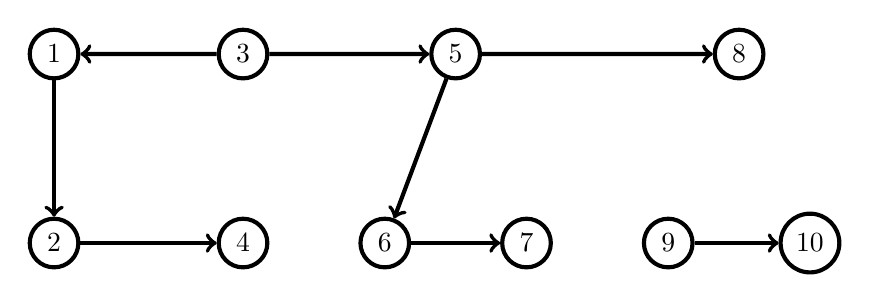
\begin{tikzpicture}[line width=1.5,scale=1.2]
 \node[circle,draw=black] (1) at (0,2) {$1$};
 \node[circle,draw=black] (2) at (0,0) {$2$};
 \node[circle,draw=black] (3) at (2,2) {$3$};
 \node[circle,draw=black] (4) at (2,0) {$4$};
 \node[circle,draw=black] (5) at (4.25,2) {$5$};
 \node[circle,draw=black] (6) at (3.5,0) {$6$};
 \node[circle,draw=black] (7) at (5,0) {$7$};
 \node[circle,draw=black] (8) at (7.25,2) {$8$};
 \node[circle,draw=black] (9) at (6.5,0) {$9$};
 \node[circle,draw=black] (10) at (8,0) {$10$};
		
 \draw[->] (1) edge (2);
 \draw[->] (2) edge (4);
 \draw[->] (3) edge (1) (3) edge (5);
 \draw[->] (5) edge (6) (5) edge (8); 
 \draw[->] (6) edge (7);
 \draw[->] (9) edge (10);
\end{tikzpicture}
\end{center} 
\end{bsp} 

\begin{bem}
		Wir bezeichnen die Tiefensuche kurz als $\cc{TS}$, die vollständige Tiefensuche als $\cc{VTS}$ und die Intialisierung der Tiefensuche als $\cc{TSI}$. 
\end{bem} 

\begin{lem} \label{ts:key:lemma} 
	Sei $D=(V,A)$ Digraph, sei $s \in V$ und man betrachte die Ausführung von $\cc{TS}(s)$ nach einer Initialisierung der Tiefensuche für $D$. Während der Ausführung ist  nach jeder Knotenfärbung  Folgendes erfüllt:
	\begin{enuma} 
		\item Die Menge der grauen Knoten bildet einen gerichteten Weg $(u_0,\ldots,u_m)$ in $D_\pi$, der im Knoten $u_0=s$ beginnt. 
		\item Der Kontrollfluss befindet sich im Aufruf von $\cc{TS}(u_m)$. 
		\item Für jedes $i=1,\ldots,m$ wurde $\cc{TS}(u_i)$  aus $\cc{TS}(u_{i-1})$ aufgerufen und die Aufrufe $\cc{TS}(u_1),\ldots,\cc{TS}(u_m)$ sind noch nicht zu Ende ausgeführt. 
	\end{enuma} 
	Darüber hinaus gilt: ein Knoten $v$ wird während Ausführung genau dann entdeckt, wenn in $D$ ein $(s,v)$-Pfad existiert. 
\end{lem} 
\begin{proof}
	Für Behauptungen (a)--(c) benutzen wir die Induktion über die Anzahl der Färbungen während der Ausführung von $\cc{TS}(s)$. Die erste Färbung ist die Färbung von $s$ mit Grau. In diesem Moment der Ausführung gilt die Behauptung für  den Weg der Länge $0$, der aus dem Knoten $s$ besteht. Angenommen, die Behauptungen gelten nach $k \in\N$ Färbungen. Man betrachten den Pfad $(u_0,\ldots,u_m)$, für den die Behauptungen gelten. 
	
	Wird während der Ausführung von $\cc{TS}(u_m)$, ein weißer Knoten $v$ entdeckt, so wird $\cc{TS}(v)$ aufgerufen, in der $v$ grau gefärbt wird, sodass nach $k+1$ Färbungen die Behauptung für den Pfad $(u_0,\ldots,u_m,v)$ erfüllt wird. 
	
	Sind während der Ausführung von $\cc{TS}(u_m)$ alle von $u_m$ ausgehende Kanten sondiert, so wird $u_m$ schwarz gefärbt, die Ausführung von $\cc{TS}(u_m)$ terminiert und der Kontrollfluss kehrt zum Aufruf $\cc{TS}(u_{m-1})$. In diesem Fall gelten die Behauptungen nach $k+1$ Färbungen für den Pfad $(u_0,\ldots,u_{m-1})$. 
	
	Nun zeigen wir die letzte Behauptung: wenn ein Knoten $v$ entdeckt wird, dann bilden laut der Behauptung (a) die Knoten, die im Moment der Entdeckung von $v$ grau sind, einen $(s,v)$-Pfad. Umgekehrt, sei $v \in V$ ein Knoten, für welchen ein $(s,v)$-Pfad $(v_0,\ldots,v_t)$ in $D$ existiert. Wir zeigen, dass der Knoten $v$ entdeckt. Angenommen, das wäre falsch. Wir zeigen durch Induktion über $i=1,\ldots,t$, dass der Knoten $v_i$ entdeckt wird. Der Knoten $v_0=s$ wird entdeckt. Sei also $1 \le i < t$ und wir nehmen an, dass $v_0,\ldots,v_{i-1}$ entdeckt werden. Da $v_{i-1}$ entdeckt wird, wird die Kanten $(v_{i-1},v_i)$ sondiert, sodass $v_i$ spätestens beim Sondieren der Kante $(v_{i-1},v_i)$ entdeckt wird. 
\end{proof} 

\begin{kor} \label{kor:weisse:pfade} 
	Sei $D=(V,A)$ Digraph und sei $u \in V$.
	Sind die Farbattribute der Knoten von $V$ auf weiß/grau/schwarz gesetzt, und ist $u$ ein weißer Knoten, für den man $\cc{TS}(u)$ startet, so wird ein weißer Knoten $v \in V$ während der Ausführung von $\cc{TS}(u)$ genau dann entdeckt, wenn vor der Ausführung von $\cc{TS}(u)$ ein $(u,v)$-Pfad aus weißen Knoten existiert. 
\end{kor} 
\begin{proof}
	Bei der Ausführung von $\cc{TS}(u)$, wird die TS für Knoten, die vor der Ausführung grau oder schwarz waren, nicht aufgerufen. Somit entspricht der Ausführung von $\cc{TS}(u)$ einer Ausführung auf dem Teilgraphen von $D$, der durch Knoten induziert ist, welche vor der Ausführung weiß waren. Die Behauptung folgt also aus der letzten Behauptung von Lemma~\ref{ts:key:lemma}. 
\end{proof} 

\begin{lem}
	Sei $D= (V,A)$ Digraph. 
	Nach der Initialisierung der Tiefensuche und während der Ausführung von der vollständige Tiefensuche der Graph $D_\pi$ stets ein gerichteter Wald. Die Wurzel der Bäume dieses Waldes sind genau die Knoten $u \in V$, für welche $\cc{TS}(u)$ direkt aus der vollständigen Tiefensuche aufgerufen wurde. 
\end{lem} 
\begin{proof} 
	Die Anzahl der Knoten, die während der Ausführung entdeckt werden nimmt während der Ausführung zu. Am Anfang der Ausführung wird der Knoten $s$ entdeckt und grau gefärbt. Die Behauptung gilt also am Anfang der Ausführung. Wir führen Induktion nach der Anzahl der Färbungen mit der Farben Grau. Am Anfang ist kein Knoten grau gefärbt und kein Vorgänger gesetzt, sodass $D_\pi$ ein Wald ohne Kanten ist. 
\end{proof} 

\begin{thm} \label{thm:ts:und:zyklen} 
	Sei $D=(V,A)$ Digraph, sei $s \in V$ und man betrachte die Ausführung von $\cc{TS}(s)$ nach einer Initialisierung der Tiefensuche für $D$. Der Digraph $D$ enthält genau dann einen von $s$ aus erreichbaren Zyklus, wenn während der Ausführung beim Sondieren einer der Kanten $(u,v)$ die Farbe von $v$ grau ist. 
\end{thm}
\begin{proof}	
	Sei während der Ausführung beim Sondieren eine Kante $(u,v)$ die Farbe von $v$ grau. Nach Lemma~\ref{ts:key:lemma} bildet die Menge der Knoten, die Grau gefärbt sind einen $(s,u)$-Weg $(u_0,\ldots,u_m)$ mit $u_0=s$ und $u=u_m$. Der Knoten $v$ ist also ein Knoten $u_j$ auf diesem Weg. Somit ist $(u_j,\ldots,u_m,u_j)$ ein Zyklus in $D$. 
	
	Umgekehrt sei $Z$ ein Zyklus, der von $s$ aus durch einen Pfad erreichbar ist. Wir zeigen, dass während der bei der Sondierung einer Kante der Endknoten der Kante grau ist. Sei $u$ der Knoten im Zyklus $Z$, der während der Ausführung unter allen Knoten von $Z$ als erster entdeckt wird. Nach der Färbung von $u$ mit Grau existiert nach Lemma~\ref{ts:key:lemma} ein $(s,u)$-Pfad $(u_0,\ldots,u_m)$ mit $s=u_0$ und $u_m=u$, der keinen anderen Knoten von $Z$ außer $u$ enthält. Wir schreiben $Z$ als $(v_0,\ldots,v_t,v_0)$ mit $v_0=u$.  
	
	Unmittelbar vor der Entdeckung ist $v_0,\ldots,v_t$ ein Pfad aus weißen Knoten. Nach Korollar~\ref{kor:weisse:pfade} wird während der Ausführung von $\cc{TS}(u)$ der Knoten $v_t$ entdeckt. Wir wenden das Lemma~\ref{ts:key:lemma} zum Teilgraphen an, der durch die Knoten induziert wird, die unmittelbar vor der Entdeckung von $u$ weiß sind. Da  $(v_0,\ldots,v_t)$ ein Pfad in diesem Teilgraphen ist, wird $v_t$ während der Ausführung von $\cc{TS}(u)$ entdeckt. Bei der Entdeckung von $v_t$ gibt es zwei Arten von grauen Knoten.  Die Knoten, welche vor dem Aufruf von $\cc{TS}(u)$ grau gefärbt wurden, sind $u_0,\ldots,u_m$. Die Knoten, die während der Ausführung von $\cc{TS}(u)$ und bis zum Aufruf von $\cc{TS}(v_t)$ grau gefärbt wurden, bilden einen $(u,v_t)$-Weg. 
	
	Es folgt:  nach der Entdeckung von $v_t$ hat der Weg aus grauen Knoten die Form $(u_0,\ldots,u_m, w_1,\ldots,w_\ell)$ mit $w_\ell =v_t$ hat. Beim sondieren der Kante $(v_t,u)$ ist also die Farbe von $u=u_m$ grau. 
\end{proof}

\begin{defn}
	Bzgl. einer vollständigen Tiefensuche auf $D=(V,A)$ mit Startknoten $s$ definieren die \textbf{Lebenszeitintervall} eines Knoten $v \in V$ als die Menge
	\[
			I_u:=\setcond{t \in \Z}{ \cc{Grau}[u] \le t \le \cc{Schwarz}[u]}. 
	\]
\end{defn} 

\begin{thm}[Klammerungstheorem]
\label{thm:klammerung}
Bei der vollständigen Tiefensuche auf einem Digraphen $D=(V,A)$ ist für jedes Paar von Knoten $u$ und $v$ genau eine der drei folgenden Bedingungen erfüllt:
\begin{enuma}

 \item $I_u \cap I_v = \emptyset$  und weder $u$ noch $v$ ist im Tiefensuchwald ein Nachfahre des anderen.

 \item $I_u \subseteq I_v$ und $u$ ist im Tiefensuchwald ein Nachfahre von $v$.

 \item $I_v \subseteq I_u$ und $v$ ist im Tiefensuchwald ein Nachfahre von $u$.

\end{enuma}
\end{thm}
\begin{proof}
	Die Aussage ist symmetrisch bzgl. $u$ und $v$. Wir  nehmen also ohne Beschränkung der Allgemeinheit an, dass während der Ausführung der vollständigen Tiefensuche der Knoten $u$ als erster entdeckt wurde. Ist die Tiefensuche für $v$ nach der Terminierung der Tiefensuche für $u$ aufgerufen worden, so gilt $I_u \cap I_v = \emptyset$. Ansonsten ist die Tiefensuche für $v$ vor der Terminierung der Tiefensuche für $u$ aufgerufen worden. Das bedeutet, dass der Knoten $v$ während der Ausführung von $u$ entdeckt worden ist. Der Aufruf von $TS(v)$ erfolgt also durch eine Folge der geschachtelten rekursiven Aufrufen 
	\[
		TS(u) \xrightarrow{} \cdots \xrightarrow{} TS(v) 
	\] 
	Somit terminiert $TS(v)$ vor $TS(u)$. Es gilt also $I_v \subseteq I_u$ ist $v$ ist Nachfahre von $u$. 
\end{proof}


\begin{bsp} 
	Die Relation der Lebenszeit Intervallen zu einander kann durch geklammerte Ausdrücke dargestellt werden. 
	Zur Illustration dieses Zusammenhangs sehen wir uns wieder die Tiefensuche aus Beispiel~\ref{bsp:tiefensuche} an.
	Die Daten der Zeitstempel sind in folgender Tabelle zusammengefasst:
	\begin{table}[H]
		\centering
		\begin{tabular}{|c|c|c|c|c|c|c|c|c|c|c|}
			\hline
			\textbf{Knoten $u$}        & \textbf{1} & \textbf{2} & \textbf{3} & \textbf{4} & \textbf{5} & \textbf{6} & \textbf{7} & \textbf{8} & \textbf{9} & \textbf{10} \\ \hline
			\textbf{$\cc{Grau}[u]$}    & 2          & 3          & 1          & 4          & 8          & 9          & 10         & 13         & 17         & 18          \\ \hline
			\textbf{$\cc{Schwarz}[u]$} & 7          & 6          & 16         & 5          & 15         & 12         & 11         & 14         & 20         & 19          \\ \hline
		\end{tabular}
	\end{table}
	Nach obiger Vorschrift können wir damit den zugehörigen Klammerausdruck
	\[
	(3\ (1\ (2\ (4\ 4)\ 2)\ 1)\ (5\ (6\ (7\ 7)\ 6)\ (8\ 8)\ 5)\ 3)\ (9\ (10\ 10)\ 9)
	\]
	ablesen.
	
	Eine andere Möglichkeit diese Klammerstruktur auszudrücken ist im folgenden Satz festgehalten:
\end{bsp} 


\begin{bem}
Als direkte Konsequenz des Klammerungstheorems erhalten wir eine Charakterisierung der Nachfahren im Tiefensuchwald eines gegebenen Knotens.
\end{bem} 

\begin{kor}
\label{cor:nachfahre-tiefenwald}
Der Knoten $v$ ist in einem Tiefensuchwald eines Digraphen genau dann ein echter Nachfahre eines Knotens $u$, wenn
\[
\cc{Grau}[u] < \cc{Grau}[v] < \cc{Schwarz}[v]  < \cc{Schwarz}[u].
\]
\end{kor}

\begin{bem} 
Eine alternative Charakterisierung der Nachfahreneigenschaft in Tiefensuchwäldern, die allerdings über die Farben der Knoten während der Suche geht, wird uns später bei den Anwendungen der Tiefensuche nützlich sein. 
\end{bem}


\begin{defn}
\label{def:kantenarten-tiefensuche}
Die Kanten $(u,v) \in A$ die bei einer Tiefensuche auf $D=(V,A)$ sondiert werden, werden in Abhängigkeit davon, welche Farbe $v$ beim Sondieren von $(u,v)$ hat und in welchem Zusammenhang $\cc{Grau}[u]$  und $\cc{Grau}[v]$ stehen, in die folgenden Arten unterteilt: 
\begin{center} 
\begin{tabular}{l|l}
	Art von $(u,v) \in A$ & Bedingung beim Sondieren 
	\\ \hline 
	\textbf{Baumkante} & $\cc{Farbe}[v]=\cc{weiss}$ 
\\	\textbf{Rückwärtskante} & $\cc{Farbe}[v] = \cc{grau}$
\\ \textbf{Vorwärtskante} & $\cc{Farbe}[v] = \cc{schwarz}$, $\cc{Grau}[u] < \cc{Grau}[v]$
\\ \textbf{Querkante} & $\cc{Farbe}[v] = \cc{schwarz}$, $\cc{Grau}[u] > \cc{Grau}[v]$
\end{tabular} 
\end{center} 
Baumkanten sind die Kanten des Tiefensuchwalds $D_\pi$. 
\end{defn}

\begin{bsp} Im Fall der Adjazensliste 
	\begin{align*}
		 1: & \ [2,4] 
		 \\ 2: & \  [3,4]
		 \\ 3: & \ [1]
		 \\  4: & \ [3]
	\end{align*}
 wird  während der Ausführung von $\cc{Tiefensuche}(1)$ die folgende Unterteilung der Kanten in die vier Arten festgelegt: 
	\begin{center} 
	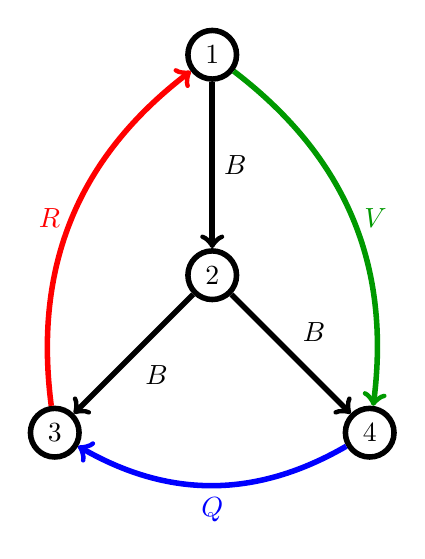
\begin{tikzpicture}[line width=2,scale=2]
		\node[circle,draw=black] (1) at (0,3.4) {$1$};
		\node[circle,draw=black] (2) at (0,2) {$2$};
		\node[circle,draw=black] (3) at (-1,1) {$3$};
		\node[circle,draw=black] (4) at (1,1) {$4$};
		\draw[->] (1) edge node[right]{$B$}(2) (2) edge node[below right]{$B$} (3) (2) edge node[above right]{$B$} (4);
		\draw[->,red] (3) edge[bend left] node[left]{$R$} (1);
		\draw[->,green!60!black]  (1) edge[bend left] node[right]{$V$} (4);
		\draw[->,blue] (4) edge[bend left] node[below]{$Q$} (3);
	\end{tikzpicture} 
	\end{center} 
\end{bsp} 

\begin{prop} 
	Wird die Unterteilung der Kanten in die vier Arten Baum-, Rückwärts- Vorwärts- und Querkante im Rahmen der vollständigen Tiefensuche durchgeführt, so ist jede Kante, welche zwei Bäume des Tiefensuchbaums verbindet eine Querkante. 
\end{prop} 


%\begin{remark}
%Durch die TS können die Kanten $(u,v)$ des Graphen in drei Arten klassifiziert werden: die Vorwärtskanten (beim sondieren von $(u,v)$ ist $v$ weiß), die Rückwärtskarten (beim sondieren der Kante ist $v$ grau) und die Querkanten (beim Sondieren der Kante ist $v$ schwarz). Die Menge aller  $\{u,v\}$ derart, dass $(u,v) \in E$ als ein Vorwärtskante klassifiziert wurde, ist Kantenmenge eines Baums. Die Knotenmenge dieses Baums ist die Menge aller entdeckten Knoten.
%\end{remark}

\begin{bsp} 
Wir schauen uns wiederum die Tiefensuche aus Beispiel~\ref{bsp:tiefensuche} an und, basierend auf den bereits erhobenen Daten, stellen wir die Klassifikation der Kanten des bearbeiteten Digraphen farbkodiert in folgender Abbildung dar.
Dabei sind Baumkanten schwarz, Rückwärtskanten rot, Vorwärtskanten blau und Querkanten grün markiert.

\begin{center} 
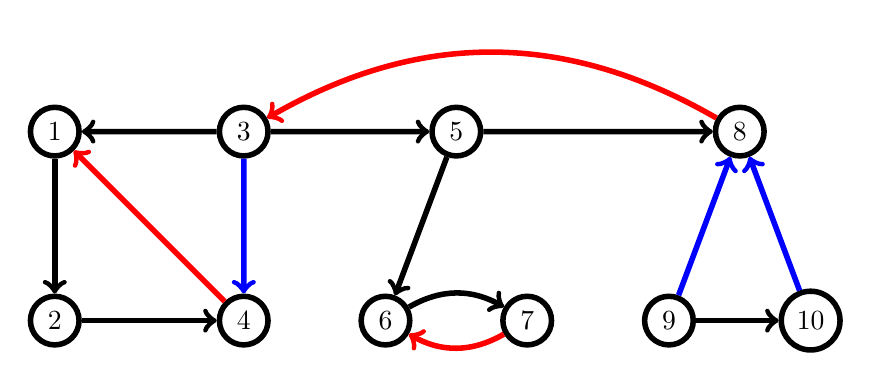
\begin{tikzpicture}[line width=2,scale=1.2]
 \node[circle,draw=black] (1) at (0,2) {$1$};
 \node[circle,draw=black] (2) at (0,0) {$2$};
 \node[circle,draw=black] (3) at (2,2) {$3$};
 \node[circle,draw=black] (4) at (2,0) {$4$};
 \node[circle,draw=black] (5) at (4.25,2) {$5$};
 \node[circle,draw=black] (6) at (3.5,0) {$6$};
 \node[circle,draw=black] (7) at (5,0) {$7$};
 \node[circle,draw=black] (8) at (7.25,2) {$8$};
 \node[circle,draw=black] (9) at (6.5,0) {$9$};
 \node[circle,draw=black] (10) at (8,0) {$10$};

% Baumkanten
 \draw[->] (1) edge (2);
 \draw[->] (2) edge (4);
 \draw[->] (3) edge (1) (3) edge (5);
 \draw[->] (5) edge (6) (5) edge (8); 
 \draw[->] (6) to[bend left] (7);
 \draw[->] (9) edge (10);

% Rückwärtskanten
 \draw[->,red] (4) edge (1);
 \draw[->,red] (7) to[bend left] (6);
 \draw[->,red] (8) to[bend right] (3);

% Vorwärtskanten
 \draw[->,blue] (3) edge (4);
 \draw[->,blue] (9) edge (8);
 \draw[->,blue] (10) edge (8); 
	
% Querkanten (keine vorhanden..)
	
\end{tikzpicture}
\end{center} 
\end{bsp} 


\begin{thm}
Bei einer Tiefensuche auf einem ungerichteten Graphen $G$ ist jede Kante entweder eine Baumkante oder eine Rückwärtskante.
\end{thm}

\begin{proof}
Sei $(u,v)$ eine beliebige Kante von~$G$ und seien die Knoten so bezeichnet, dass $\cc{Grau}[u] < \cc{Grau}[v]$ gilt.
Die Tiefensuche muss daher den Knoten~$v$ entdeckt und fertig abgearbeitet haben, bevor~$u$ fertig abgearbeitet ist.
In der Zwischenzeit ist der Knoten~$u$ stets grau.
Falls die Durchmusterung die Kante zuerst in der Richtung von~$u$ nach~$v$ sondiert, so ist~$v$ bis dahin unentdeckt (also weiß) gewesen, da die Kante sonst bereits in Gegenrichtung sondiert worden wäre.
Mit anderen Worten, die Kante $(u,v)$ ist eine Baumkante.

Falls nun die Durchmusterung die Kante zuerst in der Richtung von~$v$ nach~$u$ sondiert, so ist die Kante $(u,v)$ eine Rückwärtskante, da~$u$ zu dem Zeitpunkt der Sondierung noch grau ist.
\end{proof}


\begin{bem}
	Analog zur diskutierten Breitensuche kann man eine \emph{Tiefensuche} auch ohne Rekursion umsetzen.
	Dies hat praktische Vorteile, weil der Programmstack nicht  belastet wird.
	Dazu ersetzt man die Warteschlange $Q$ durch einen sogenannten \emph{Stack} ($=$ \emph{Stapel}). Für die Tiefensuche kann ein Stack auf der Basis von einem Array umgesetzt werden. 
	
	Hier eine ziemlich direkte Konvertierung der rekursiven Umsetzung. Wir gehen von einem zugrundeliegenden Stack $S$ aus. Als $\cc{Top}(S)$ bezeichnen wir das oberste Element des Stacks . Durch $\cc{Pop}(S)$ erfolgt die Entfernung und Rückgabe des obersten Elements. Durch $\cc{Push}(S,u)$ wird ein neues Element $u$ auf den Stack gelegt. Die Elemente $N[u]$ indexieren wir mit Zahlen $0$ bis $\deg(u)-1$, wobei hier $\deg(u)$ der Grad des Knotens $u$ ist. Wir führen ein Array $\cc{ind}$ ein, in dem durch $\cc{ind}[u]$ notiert wird, dass beim Sondieren der Nachbarn von $u \in V$  der Knoten $v=N[u][\cc{ind}[u]]$ als  nächster dran ist. Ist $\cc{ind}[u]= \deg(u)$, so hat man alle Nachbarn von $u$ sondiert. Wir setzen am Anfang $\cc{ind}[u]=0$ für alle $u \in V$, färben den Startknoten $s$ grau und legen $s$ auf $S$. Auf diese Weise lassen sich mit Hilfe von $S$ und $\cc{ind}$ die gerade laufenden rekursiven Aufrufe der Tiefensuche simulieren: 
	
	\begin{algorithm}[H]
		\caption{$\cc{Tiefensuche-mit-Stack}(s)$} 
		\begin{algorithmic}[1]
			\STATE Stack $S$ für höchstens $|V|$ Elemente anlegen
			\STATE $\cc{Farbe}[s] = \cc{grau}$ 
			\STATE $\cc{push}(S,s)$
			\STATE Liste $\cc{Ind}$  mit $\cc{Ind}[u]=0$ für alle $u \in V$ anlegen
			\WHILE{$S$ nicht leer }
			\STATE $u:= \cc{top}(S)$ \quad \COMMENT{Suche für $u$ läuft weiter}
			\IF{$\cc{ind}[u] = \deg(u)$} 
			\STATE $\cc{pop}(S)$   \quad \COMMENT{Suche für $u$ wird beendet}
			\STATE $\cc{Farbe}[u] := \cc{schwarz}$
			\ELSE
			\STATE $v=N[u][\cc{ind}[u]]$ \quad \COMMENT{Sondierung der Nachbarn von $u$ wird fortgesetzt} 
			\STATE $\cc{ind}[u]:=\cc{ind}[u]+1$				
			\IF{$\cc{Farbe}[v] = \cc{weiss}$}
			\STATE $\cc{Farbe}[v] = \cc{grau}$ \quad \COMMENT{Neuer Knoten ist entdeckt}
			\STATE $\cc{push}(S,v)$ \quad \COMMENT{Suche für $v$ wird gestartet}
			\ENDIF 
			\ENDIF 
			\ENDWHILE  
		\end{algorithmic}
	\end{algorithm}
	
	Die weiteren Daten, die man im Rahmen der rekursiven Tiefensuche berechnen kann, kann man auch in der obigen iterativen Version an den entsprechenden Stellen berechnen. 
\end{bem}

\begin{bem}\ Umsetzung: 
\lstinputlisting{Code/dfs.sage}
\end{bem} 


\condclearpage
\subsection{Anwendung I -- Topologisches Sortieren}

\begin{defn} 
Sei $D=(V,A)$ ein Digraph mit $n$ Knoten.
Eine \emph{topologische Sortierung} von $D$ ist eine Anordnung $v_1,\ldots,v_n$ seiner Knoten, so dass $i < j$ gilt, falls $(v_i,v_j) \in A$ eine Kante in~$D$ ist.
Das heißt, der Startknoten einer jeden Kante kommt in der Anordnung vor dem Endknoten.
\end{defn} 

\begin{bem}
Man kann die topologische Sortierung auch als horizontale Anordnung der Knoten von~$D$ auffassen, so dass jede Kante von links nach rechts zeigt.

Diese Veranschaulichung zeigt, dass es nicht möglich ist, einen Digraphen topologisch zu sortieren, wenn er einen Zyklus enthält.
Im Folgenden werden wir sehen, wie man mit einer Tiefensuche jeden \emph{azyklischen} Digraphen topologisch sortieren kann.
Als Konsequenz ergibt sich:
\end{bem} 

\begin{prop}
Ein Digraph besitzt genau dann eine topologische Sortierung, wenn er azyklisch ist.
\end{prop}

\begin{bem}
	Eine Anwendung des topologischen Sortierens ist \textbf{makefile}. Die Kanten des Diagraphen sind durch  die Paare target-prerequisite gegeben. Die targets sollen in einer topologisch sortierten Reihenfolge abgearbeitet werden. 
	
	Eine andere Anwendung ist das Sequenzieren von Aufträgen (engl.~\emph{scheduling}).
\end{bem}


\begin{thm}
	Nach der Ausführung der vollständigen Tiefensuche auf einem azyklischen Digraphen $D=(V,A)$ ist die Anordnung der Knoten $u \in V$ in der absteigenden Reihenfolge nach $\cc{Schwarz}[u]$ eine topologische Sortierung. Diese Anordnung kann während der Tiefensuche in der Zeit $\Theta(|V|+|A|)$ berechnet werden. 
\end{thm}

\begin{proof}
	Wir betrachten eine Kante $(u,v)$. Ist $v$ vor $u$ entdeckt worden, so wird während der Ausführung von $TS(u)$ der Knoten $u$ nicht entdeckt, denn sonst gäbe es einen $(v,u)$-Pfad und somit auch einen Zyklus in $D$. Das bedeutet, dass in diesem Fall $TS(v)$ vor $TS(u)$ terminiert. Es gilt also $\cc{Schwarz}[v] \le \cc{Schwarz}[u]$. 
	
	Wird $u$ vor $v$ entdeckt, so wird $v$ während der Ausführung von $TS(u)$ spätestens beim Sondieren von $(u,v)$ entdeckt. In diesem Fall terminiert $TS(v)$ ebenfalls vor $TS(u)$. Somit gilt auch in diesem Fall $\cc{Schwarz}[v] \le \cc{Schwarz}[u]$.
\end{proof}




\subsection{Anwendung II -- Starke Zusammenhangskomponenten}

\begin{defn}
	Knoten $u,v \in V$ eines Digraphen $D=(V,A)$ heißen \textbf{gegenseitig erreichbar} wenn ein $(u,v)$-Pfad sowie ein $(v,u)$-Pfad existiert. Gegenseitige Erreichbarkeit ist eine Äquivalenzrelation auf $V$. Die Äquivalenzklassen bzgl. dieser Relation nennt man \textbf{starke Zusammenhangskomponenten} (SZK) von $D$. 
\end{defn} 

\begin{bsp}
	In diesem Beispiel sind die starkten Zusammenhangskomponenten mit mehr als einem Knoten farbich hinterlegt: 
\begin{center}
	\includegraphics[width=0.5\textwidth]{Code/strongly_connected_comp.pdf}
\end{center} 
\end{bsp}

\begin{thm}
	\label{thm:starke-zshgk-laufzeit}
	Ist ein Digraph $D=(V,A)$ als Adjazenzliste gegeben, so hat der Algorithmus aus \ref{szk:algo} die Laufzeit $\Theta(|V|+|A|)$.
\end{thm}
\begin{proof}
	Die Berechnung von $D^\top$ sowie die beiden vollständigen Tiefensuchen sind benötigen jeweils  $\Theta(|V|+|A|)$ Elementaroperationen. 
\end{proof}

\begin{defn}
	Der \textbf{Komponentengraphen} $D^K=(V^K,A^K)$ eines Digraphen $D=(V,A)$
	ist ein Digraph, beim dem die Menge $V^K$ die Menge von SZK von $D$ ist und die Menge $A^K$ der Kanten die Menge aller paare $(U,W)$ mit $U,W \in V^K$ mit der Eigenschaft, dass  $(u,w) \in A$  für ein $u \in U$ und $w \in W$  erfüllt ist. 
\end{defn}

\begin{prop}
	Der Komponentengraph eines jeden Digraphen ist azyklisch. 
\end{prop}


\begin{bsp}
	\label{bsp:starke-zusammenhangskomponenten}
	Die starken Zusammenhangskomponenten des Digraphen aus Beispiel~\ref{bsp:tiefensuche} bestehen aus den Knoten gleicher Farbe in folgender Abbildung:
	
	\hfill
	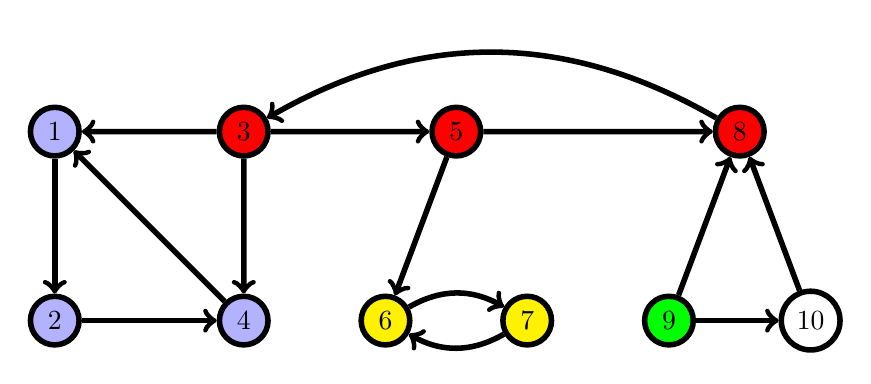
\begin{tikzpicture}[line width=2,scale=1.2]
		\node[fill=blue!30!white,circle,draw] (1) at (0,2) {$1$};
		\node[fill=blue!30!white,circle,draw] (2) at (0,0) {$2$};
		\node[fill=red,circle,draw] (3) at (2,2) {$3$};
		\node[fill=blue!30!white,circle,draw] (4) at (2,0) {$4$};
		\node[fill=red,circle,draw] (5) at (4.25,2) {$5$};
		\node[fill=yellow,circle,draw] (6) at (3.5,0) {$6$};
		\node[fill=yellow,circle,draw] (7) at (5,0) {$7$};
		\node[fill=red,circle,draw] (8) at (7.25,2) {$8$};
		\node[fill=green,circle,draw] (9) at (6.5,0) {$9$};
		\node[circle,draw=black] (10) at (8,0) {$10$};
		
		\draw[->] (1) edge (2);
		\draw[->] (2) edge (4);
		\draw[->] (3) edge (1) (3) edge (4) (3) edge (5);
		\draw[->] (4) edge (1);
		\draw[->] (5) edge (6) (5) edge (8); 
		\draw[->] (6) to[bend left] (7);
		\draw[->] (7) to[bend left] (6);
		\draw[->] (8) to[bend right] (3);
		\draw[->] (9) edge (8) (9) edge (10);
		\draw[->] (10) edge (8); 
	\end{tikzpicture}
	\hfill\,
\end{bsp}

Der Komponentengraph dieses  Digraphen ist: 
\begin{center} 
	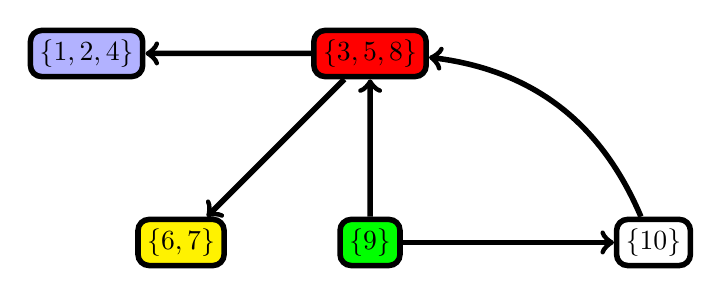
\begin{tikzpicture}[line width=2,scale=1.2]
		\node[fill=blue!30!white,rounded corners,draw] (1) at (3,2) {$\{1,2,4\}$};
		% \node[fill=blue,rounded corners,draw] (2) at (0,0) {$2$};
		% \node[fill=red,rounded corners,draw] (3) at (2,2) {$3$};
		% \node[fill=blue,rounded corners,draw] (4) at (2,0) {$4$};
		\node[fill=red,rounded corners,draw] (5) at (6,2) {$\{3,5,8\}$};
		\node[fill=yellow,rounded corners,draw] (6) at (4,0) {$\{6,7\}$};
		% \node[fill=yellow,rounded corners,draw] (7) at (5,0) {$7$};
		% \node[fill=red,rounded corners,draw] (8) at (7.25,2) {$8$};
		\node[fill=green,rounded corners,draw] (9) at (6,0) {$\{9\}$};
		\node[rounded corners,draw=black] (10) at (9,0) {$\{10\}$};
		
		\draw[->] (5) edge (6) (5) edge (1); 
		\draw[->] (9) edge (5) (9) edge (10);
		\draw[->] (10) to[bend right] (5); 
	\end{tikzpicture}
\end{center}


\begin{defn}
	Für einen Digraphen $D = (V,A)$ führen wir den sogenannten
 \emph{transponierten Graphen} $D^\top = (V,A^\top)$ mit $A^\top = \{(u,v) \in V \times V : (v,u) \in A\}$ ein. 
Wir erhalten also $D^\top$ aus $D$, indem wir die Orientierung aller Kanten von $D$ umdrehen.
\end{defn} 


\begin{prop}
\label{beob:d-vs-dt}
Der zu einem Digraphen $D=(V,A)$ transponierte Graph $D^\top$ hat dieselben starken Zusammenhangskomponenten wie~$D$.
\end{prop}

\begin{bem}  \label{szk:algo}
	Sei $D = (V,A)$ Digraph. Zur Berechnung der SZK von $D$ kann der folgende Algorithmus benutzt werden, den wir als $\cc{SZK}(D)$ bezeichnen: 
\begin{itemize}
	\item \textbf{Phase~1: Anordnung.} Ordne mit Hilfe der vollständigen Tiefesuche auf $D$ die Knotenmenge $V$ in absteigender Reihenfolge $u_1,\ldots,u_n$ der Abarbeitungszeit ($n:=|V|$). Es reicht dafür beim Abarbeiten eines Knoten, den Knoten zu einer Liste mit $n$ Elementen hinzuzufügen (und die Liste vom Ende beginnend zu füllen). 
	\item \textbf{Phase~2: Berechnung der Komponenten.} Für eine vollständige Tiefensuche auf $D^
\top$ durch, bei der  über die Knoten $u \in V$ in der oben bestimmten Reihenfolge $u_1,\ldots,u_n$ iteriert wird. Dabei entdeckt jeder Aufruf der Tiefensuche aus der vollständigen Tiefensuche die Knoten einer starken Zusammenhangskomponente.
\end{itemize} 

Wie man Phase~2 genau umsetzt hängt unter anderem davon ab, in welchem Format man die SZK speichern möchte. 
\end{bem} 

\begin{bem} Umsetzung: 
\lstinputlisting{Code/szk.sage}
\end{bem} 


\begin{thm}
$\cc{SZK}(D)$ bestimmt die starken Zusammenhangskomponenten eines Digraphen~$D=(V,A)$ korrekt.
\end{thm}


\begin{bem}
	Die Präsentation der Tiefensuche basiert auf  \cite{CLRS17}.
\end{bem}  

\section{Der Prim-Algorithmus}


\begin{bem}
In diesem Abschnitt sei $G=(V,E)$ ein (ungerichteter) Graph und $w : E \to \R$ eine \textbf{Gewichtsfunktion} auf seinen Kanten.
Das hei\ss t, jeder Kante $\{u,v\} \in E$ wird eine Zahl (ihr \textbf{Gewicht}) $w(u,v) \in \R$ zugeordnet.
Das Tripel $G=(V,E,w)$ hei\ss t dann \textbf{gewichteter Graph}.
Wir nehmen im Folgenden stets an, dass der Graph~$G$ \underline{zusammenhängend} ist.

Um die Gewichtsfunktion in die Adjazenzliste von $G$ aufzunehmen, kann man die Nachbarn $N[u]$ eines Knotens $u \in V$ zum Beispiel als Paare $(v,w(u,v)) \in V \times \R$ führen.
\end{bem}

\begin{defn}
Sei $G=(V,E,w)$ ein gewichteter Graph.
Ein Baum $T=(V',E')$ heißt \textbf{Spannbaum} von~$G$, falls $V=V'$ und $E' \subseteq E$ gelten.
Für jeden Teilgraphen $G' = (V',E')$ von~$G$ definieren wir sein \textbf{Gewicht} als
\[
w(G') := \sum_{e \in E'} w(e).
\]
%
Ein Spannbaum $T=(V,E')$ von~$G$ heißt \textbf{minimaler Spannbaum}, wenn~$T$ unter allen Spannbäumen von~$G$ minimales Gewicht hat.
\end{defn} 


\begin{bsp}
Jeder Breitensuchbaum und jeder Tiefensuchbaum ist ein Spannbaum.
Im Allgemeinen sind diese Spannbäume aber keine \underline{minimalen} Spannbäume:\\[1em]

\hfill
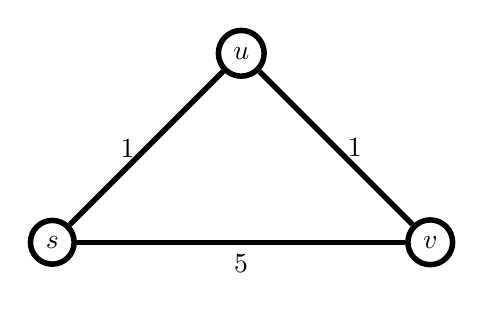
\begin{tikzpicture}[line width=2,scale=1.2]
	 \node[circle,draw=black] (s) at (0,0) {$s$};
	 \node[circle,draw=black] (u) at (2,2) {$u$};
	 \node[circle,draw=black] (v) at (4,0) {$v$};
	 \draw[-] (s) edge node[midway,left]{$1$} (u);
	 \draw[-] (u) edge node[midway,right]{$1$} (v);
	 \draw[-] (v) edge node[midway,below]{$5$} (s);
\end{tikzpicture}
\hfill\,


\end{bsp}

\begin{prop}
Sei $G=(V,E,w)$ ein gewichteter Graph mit paarweise verschiedenen Kantengewichten, das hei\ss t, für je zwei Kanten $\{u,v\} \neq \{r,s\}$ von~$G$ gilt $w(u,v) \neq w(r,s)$.
Dann gibt es genau einen minimalen Spannbaum in~$G$.
\end{prop}
\begin{proof}
Angenommen, es gibt zwei verschiedene minimale Spannbäume $S$ und $T$ von~$G$.
Dann gibt es mindestens eine Kante $e \in E$, die in $S \setminus T$ oder in $T \setminus S$ liegt.
Sei $e_1$ unter allen solchen Kanten, die Kante kleinsten Gewichts, also $w(e_1) < w(e)$, für alle Kanten $e \in S \setminus T \cup T \setminus S$.
Ohne Einschränkung sei $e_1 \in S \setminus T$. (Die Kante $e_1$ ist insbesondere eindeutig.)

Da $T$ ein Spannbaum ist, enthält der Teilgraph $T \cup \{e_1\}$ einen Kreis $C$, der wiederum die Kante $e_1$ enthält.
Der Spannbaum~$S$ ist als Baum ein kreisfreier Graph, und somit gibt es eine Kante $e_2 \in C \setminus S$, und $e_2$ gehört zu~$T$.
Nach Annahme an die Kante~$e_1$, gilt $w(e_2) > w(e_1)$.

\condclearpage

Wir betrachten den Graphen $T' := T \setminus \{e_2\} \cup \{e_1\}$.
Da~$C$ der einizige Kreis in $T \cup \{e_1\}$ ist, ist $T'$ kreisfrei und es ist $|E(T')| = |E(T)| = |V|-1$.
Somit ist $T'$ wiederum ein Spannbaum von~$G$ (siehe Übungszettel).
Weiterhin gilt
\[
w(T') = w(T) - w(e_2) + w(e_1) < w(T),
\]
was im Widerspruch dazu steht, dass $T$ als minimaler Spannbaum angenommen wurde.
\end{proof}

\begin{bem} 
Unser Ziel ist es, das \textbf{Problem des minimalen Spannbaums} möglichst effizient zu lösen:
\begin{center}
\textit{Gegeben ein zusammenhängender gewichteter Graph~$G=(V,E,w)$,\\ finde einen minimalen Spannbaum von~$G$.}
\end{center}
%
\noindent Das Bestimmen eines \underline{minimalen} Spannbaums ist in verschiedenen Problemen praxisrelevant:
%
\begin{itemize}
 \item Verlegen von Glasfaserkabeln (Gewicht einer Verbindung als Funktion von Länge, Tiefe, Bodenbeschaffenheit, etc.)
% \item Bei elektronischen Schaltkreisen will man eine Menge von Kontakten verdrahten, um diese auf das gleiche Potenzial zu legen.
 \item \emph{Spanning tree protocol} (Übersendung von Paketen in einem Netzwerk).
 \item Approximationslösung für das \emph{Problem der Handlungsreisenden}.
 \item Generieren von \emph{Labyrinthen} für Spiele (siehe zB.~\url{https://de.wikipedia.org/wiki/Datei:MAZE_30x20_Prim.ogv}).
\end{itemize}
Wir legen Ihnen nahe, sich mit diesen Anwendungen selbst etwas vertraut zu machen und nachzuvollziehen, inwiefern das Finden eines minimalen Spannbaums in jedem dieser Beispiele von Nutzen ist.
\end{bem} 

\begin{thm}[Cayley]
Der vollständige Graph $K_n$ auf $n$ Knoten hat $n^{n-2}$ Spannbäume.
\end{thm}
Als Folge ist der naive algorithmische Ansatz des Enumerierens aller Spannbäume nicht effizient.


\begin{bem}
Sind alle Kantengewichte in $G=(V,E,w)$ positiv, also $w(u,v) > 0$, für alle $\{u,v\} \in E$, so ist das Problem des minimalen Spannbaums äquivalent zum Problem der Bestimmung eines zusammenhängenden Teilgraphen $G'= (V',E')$ von $G$ mit $V=V'$ und dem kleinsten Gewicht.
\end{bem}

\begin{bem} 
In der Literatur gibt es eine ganze Reihe von Algorithmen zur Lösung des Problems des minimalen Spannbaums.
Wir diskutieren hier den sogennanten \textbf{Prim-Algorithmus} der im Jahr 1957 in einer Arbeit von Robert C.~Prim erschien und zwei Jahre später von Dijkstra neu beschrieben wurde.
Beiden Autoren (und allgemein der westlichen Forschergemeinschaft) war anscheinend die Arbeit von Vojt\v{e}ch Jarn\'{i}k aus dem Jahr 1930 nicht bekannt, der die Vorgehensweise bereits lange zuvor diskutierte.
\end{bem} 

\begin{bem}
\underline{Grundidee des Prim-Algorithmus:}
Der Algorithmus basiert auf der einfachen Idee einen Spannbaum sukzessive \glqq von Null auf\grqq\ durch das Hinzufügen von Kanten kleinstmöglichen Gewichtes wachsen zu lassen.
Genauer gesagt starten wir mit einem Startbaum~$T_0$, der aus einem beliebigen Knoten~$s$ von~$G$ besteht.
Diesen erweitern wir dann durch eine zu~$s$ adjazente Kante kleinsten Gewichtes zu dem Teilbaum~$T_1$.
Im nächsten Schritt wählen wir wieder eine Kante kleinsten Gewichtes unter den verbleibenden Kanten in~$G$ aus, die zu $T_1$ hinzugefügt werden kann und dabei die Baumeigenschaft erhält.
Wir bekommen dadurch den Teilbaum~$T_2$, der nun aus zwei Kanten besteht.
Führen wir dies Schritt für Schritt weiter gelangen wir zu einem Teilbaum~$T_{|V|-1}$ der aus $|V|-1$ Kanten besteht und ein Spannbaum von~$G$ ist.
Der Clou ist nun, dass dieser Spannbaum minimales Gewicht unter allen Spannbäumen von~$G$ hat.
\end{bem} 


\begin{bsp}
\label{bsp:prim}
Gegeben sei der folgende gewichtete zusammenhängende Graph:
%
\begin{center}
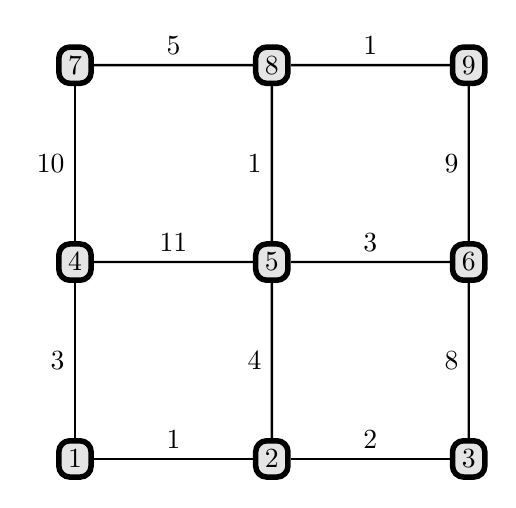
\begin{tikzpicture}[line width=2,scale=2.5]
\tikzstyle{V}=
 =[
 fill=gray!20, rounded corners, draw=black
 ]

\node[V] (1) at (0,0) {$1$};
\node[V] (2) at (1,0) {$2$};
\node[V] (3) at (2,0) {$3$};
\node[V] (4) at (0,1) {$4$};
\node[V] (5) at (1,1) {$5$};
\node[V] (6) at (2,1) {$6$};
\node[V] (7) at (0,2) {$7$};
\node[V] (8) at (1,2) {$8$};
\node[V] (9) at (2,2) {$9$};
	
\draw[line width=0.3mm] 
 (1) edge node[midway,above]{$1$} (2)  
 (2) edge node[midway,above]{$2$} (3) 
 (4) edge node[midway,above]{$11$} (5) 
 (5) edge node[midway,above]{$3$} (6) 
 (7) edge node[midway,above]{$5$} (8)
 (8) edge node[midway,above]{$1$} (9)
 (1) edge node[midway,left]{$3$} (4)
 (2) edge node[midway,left]{$4$} (5)
 (3) edge node[midway,left]{$8$} (6)
 (4) edge node[midway,left]{$10$} (7)
 (5) edge node[midway,left]{$1$} (8)
 (6) edge node[midway,left]{$9$} (9)
;
\end{tikzpicture}	
\end{center}
%
Beginnend vom Startknoten~$s=1$ illustrieren wir die Vorgehensweise des Prim-Algorithmus.
In jedem Graphen der folgenden Sequenz markieren wir den aktuellen Teilbaum~$T_i$ in rot und die in Frage kommenden Kanten für die Erweiterung zum Teilbaum $T_{i+1}$ in grün:
\begin{center}
\hfill
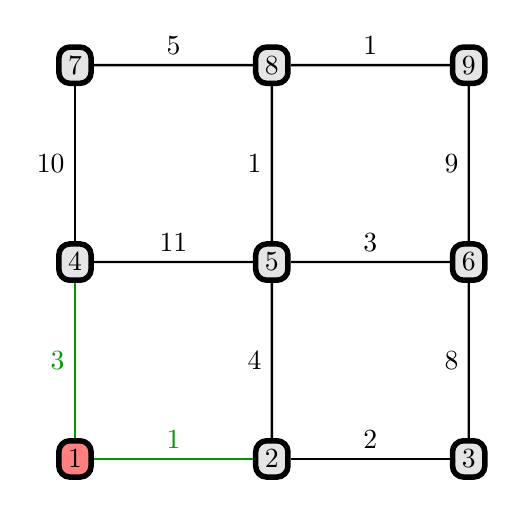
\begin{tikzpicture}[line width=2,scale=2.5]
\tikzstyle{V}=
 =[
 fill=gray!20, rounded corners, draw=black
 ]
\tikzstyle{R}=
 =[
 fill=red!50, rounded corners, draw=black
 ]

\node[R] (1) at (0,0) {$1$};
\node[V] (2) at (1,0) {$2$};
\node[V] (3) at (2,0) {$3$};
\node[V] (4) at (0,1) {$4$};
\node[V] (5) at (1,1) {$5$};
\node[V] (6) at (2,1) {$6$};
\node[V] (7) at (0,2) {$7$};
\node[V] (8) at (1,2) {$8$};
\node[V] (9) at (2,2) {$9$};
	
\draw[line width=0.3mm] 
 (1) edge[green!60!black] node[midway,above]{$1$} (2)  
 (2) edge node[midway,above]{$2$} (3) 
 (4) edge node[midway,above]{$11$} (5) 
 (5) edge node[midway,above]{$3$} (6) 
 (7) edge node[midway,above]{$5$} (8)
 (8) edge node[midway,above]{$1$} (9)
 (1) edge[green!60!black] node[midway,left]{$3$} (4)
 (2) edge node[midway,left]{$4$} (5)
 (3) edge node[midway,left]{$8$} (6)
 (4) edge node[midway,left]{$10$} (7)
 (5) edge node[midway,left]{$1$} (8)
 (6) edge node[midway,left]{$9$} (9)
;
\end{tikzpicture}	
\hfill
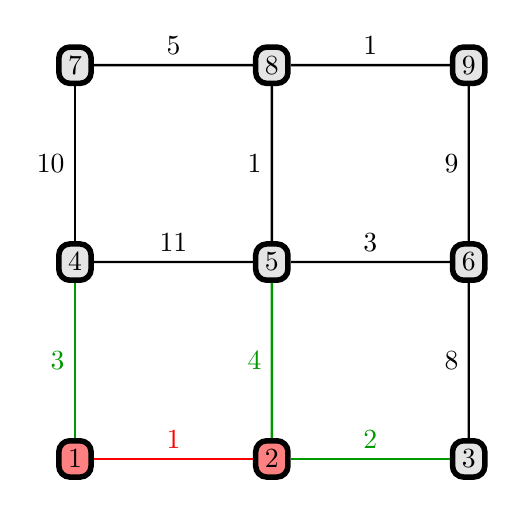
\begin{tikzpicture}[line width=2,scale=2.5]
\tikzstyle{V}=
 =[
 fill=gray!20, rounded corners, draw=black
 ]
\tikzstyle{R}=
 =[
 fill=red!50, rounded corners, draw=black
 ]

\node[R] (1) at (0,0) {$1$};
\node[R] (2) at (1,0) {$2$};
\node[V] (3) at (2,0) {$3$};
\node[V] (4) at (0,1) {$4$};
\node[V] (5) at (1,1) {$5$};
\node[V] (6) at (2,1) {$6$};
\node[V] (7) at (0,2) {$7$};
\node[V] (8) at (1,2) {$8$};
\node[V] (9) at (2,2) {$9$};
	
\draw[line width=0.3mm] 
 (1) edge[red] node[midway,above]{$1$} (2)  
 (2) edge[green!60!black] node[midway,above]{$2$} (3) 
 (4) edge node[midway,above]{$11$} (5) 
 (5) edge node[midway,above]{$3$} (6) 
 (7) edge node[midway,above]{$5$} (8)
 (8) edge node[midway,above]{$1$} (9)
 (1) edge[green!60!black] node[midway,left]{$3$} (4)
 (2) edge[green!60!black] node[midway,left]{$4$} (5)
 (3) edge node[midway,left]{$8$} (6)
 (4) edge node[midway,left]{$10$} (7)
 (5) edge node[midway,left]{$1$} (8)
 (6) edge node[midway,left]{$9$} (9)
;
\end{tikzpicture}	
\hfill\,
\end{center}
\begin{center}
\hfill
\begin{tikzpicture}[line width=2,scale=2.5]
\tikzstyle{V}=
 =[
 fill=gray!20, rounded corners, draw=black
 ]
\tikzstyle{R}=
 =[
 fill=red!50, rounded corners, draw=black
 ]

\node[R] (1) at (0,0) {$1$};
\node[R] (2) at (1,0) {$2$};
\node[R] (3) at (2,0) {$3$};
\node[V] (4) at (0,1) {$4$};
\node[V] (5) at (1,1) {$5$};
\node[V] (6) at (2,1) {$6$};
\node[V] (7) at (0,2) {$7$};
\node[V] (8) at (1,2) {$8$};
\node[V] (9) at (2,2) {$9$};
	
\draw[line width=0.3mm] 
 (1) edge[red] node[midway,above]{$1$} (2)  
 (2) edge[red] node[midway,above]{$2$} (3) 
 (4) edge node[midway,above]{$11$} (5) 
 (5) edge node[midway,above]{$3$} (6) 
 (7) edge node[midway,above]{$5$} (8)
 (8) edge node[midway,above]{$1$} (9)
 (1) edge[green!60!black] node[midway,left]{$3$} (4)
 (2) edge[green!60!black] node[midway,left]{$4$} (5)
 (3) edge[green!60!black] node[midway,left]{$8$} (6)
 (4) edge node[midway,left]{$10$} (7)
 (5) edge node[midway,left]{$1$} (8)
 (6) edge node[midway,left]{$9$} (9)
;
\end{tikzpicture}	
\hfill
\begin{tikzpicture}[line width=2,scale=2.5]
\tikzstyle{V}=
 =[
 fill=gray!20, rounded corners, draw=black
 ]
\tikzstyle{R}=
 =[
 fill=red!50, rounded corners, draw=black
 ]

\node[R] (1) at (0,0) {$1$};
\node[R] (2) at (1,0) {$2$};
\node[R] (3) at (2,0) {$3$};
\node[R] (4) at (0,1) {$4$};
\node[V] (5) at (1,1) {$5$};
\node[V] (6) at (2,1) {$6$};
\node[V] (7) at (0,2) {$7$};
\node[V] (8) at (1,2) {$8$};
\node[V] (9) at (2,2) {$9$};
	
\draw[line width=0.3mm] 
 (1) edge[red] node[midway,above]{$1$} (2)  
 (2) edge[red] node[midway,above]{$2$} (3) 
 (4) edge[green!60!black] node[midway,above]{$11$} (5) 
 (5) edge node[midway,above]{$3$} (6) 
 (7) edge node[midway,above]{$5$} (8)
 (8) edge node[midway,above]{$1$} (9)
 (1) edge[red] node[midway,left]{$3$} (4)
 (2) edge[green!60!black] node[midway,left]{$4$} (5)
 (3) edge[green!60!black] node[midway,left]{$8$} (6)
 (4) edge[green!60!black] node[midway,left]{$10$} (7)
 (5) edge node[midway,left]{$1$} (8)
 (6) edge node[midway,left]{$9$} (9)
;
\end{tikzpicture}	
\hfill\,
\end{center}
\begin{center}
\hfill
\begin{tikzpicture}[line width=2,scale=2.5]
\tikzstyle{V}=
 =[
 fill=gray!20, rounded corners, draw=black
 ]
\tikzstyle{R}=
 =[
 fill=red!50, rounded corners, draw=black
 ]

\node[R] (1) at (0,0) {$1$};
\node[R] (2) at (1,0) {$2$};
\node[R] (3) at (2,0) {$3$};
\node[R] (4) at (0,1) {$4$};
\node[R] (5) at (1,1) {$5$};
\node[V] (6) at (2,1) {$6$};
\node[V] (7) at (0,2) {$7$};
\node[V] (8) at (1,2) {$8$};
\node[V] (9) at (2,2) {$9$};
	
\draw[line width=0.3mm] 
 (1) edge[red] node[midway,above]{$1$} (2)  
 (2) edge[red] node[midway,above]{$2$} (3) 
 (4) edge node[midway,above]{$11$} (5) 
 (5) edge[green!60!black] node[midway,above]{$3$} (6) 
 (7) edge node[midway,above]{$5$} (8)
 (8) edge node[midway,above]{$1$} (9)
 (1) edge[red] node[midway,left]{$3$} (4)
 (2) edge[red] node[midway,left]{$4$} (5)
 (3) edge[green!60!black] node[midway,left]{$8$} (6)
 (4) edge[green!60!black] node[midway,left]{$10$} (7)
 (5) edge[green!60!black] node[midway,left]{$1$} (8)
 (6) edge node[midway,left]{$9$} (9)
;
\end{tikzpicture}	
\hfill
\begin{tikzpicture}[line width=2,scale=2.5]
\tikzstyle{V}=
 =[
 fill=gray!20, rounded corners, draw=black
 ]
\tikzstyle{R}=
 =[
 fill=red!50, rounded corners, draw=black
 ]

\node[R] (1) at (0,0) {$1$};
\node[R] (2) at (1,0) {$2$};
\node[R] (3) at (2,0) {$3$};
\node[R] (4) at (0,1) {$4$};
\node[R] (5) at (1,1) {$5$};
\node[V] (6) at (2,1) {$6$};
\node[V] (7) at (0,2) {$7$};
\node[R] (8) at (1,2) {$8$};
\node[V] (9) at (2,2) {$9$};
	
\draw[line width=0.3mm] 
 (1) edge[red] node[midway,above]{$1$} (2)  
 (2) edge[red] node[midway,above]{$2$} (3) 
 (4) edge node[midway,above]{$11$} (5) 
 (5) edge[green!60!black] node[midway,above]{$3$} (6) 
 (7) edge[green!60!black] node[midway,above]{$5$} (8)
 (8) edge[green!60!black] node[midway,above]{$1$} (9)
 (1) edge[red] node[midway,left]{$3$} (4)
 (2) edge[red] node[midway,left]{$4$} (5)
 (3) edge[green!60!black] node[midway,left]{$8$} (6)
 (4) edge[green!60!black] node[midway,left]{$10$} (7)
 (5) edge[red] node[midway,left]{$1$} (8)
 (6) edge node[midway,left]{$9$} (9)
;
\end{tikzpicture}	
\hfill\,
\end{center}
\begin{center}
\hfill
\begin{tikzpicture}[line width=2,scale=2.5]
\tikzstyle{V}=
 =[
 fill=gray!20, rounded corners, draw=black
 ]
\tikzstyle{R}=
 =[
 fill=red!50, rounded corners, draw=black
 ]

\node[R] (1) at (0,0) {$1$};
\node[R] (2) at (1,0) {$2$};
\node[R] (3) at (2,0) {$3$};
\node[R] (4) at (0,1) {$4$};
\node[R] (5) at (1,1) {$5$};
\node[V] (6) at (2,1) {$6$};
\node[V] (7) at (0,2) {$7$};
\node[R] (8) at (1,2) {$8$};
\node[R] (9) at (2,2) {$9$};
	
\draw[line width=0.3mm] 
 (1) edge[red] node[midway,above]{$1$} (2)  
 (2) edge[red] node[midway,above]{$2$} (3) 
 (4) edge node[midway,above]{$11$} (5) 
 (5) edge[green!60!black] node[midway,above]{$3$} (6) 
 (7) edge[green!60!black] node[midway,above]{$5$} (8)
 (8) edge[red] node[midway,above]{$1$} (9)
 (1) edge[red] node[midway,left]{$3$} (4)
 (2) edge[red] node[midway,left]{$4$} (5)
 (3) edge[green!60!black] node[midway,left]{$8$} (6)
 (4) edge[green!60!black] node[midway,left]{$10$} (7)
 (5) edge[red] node[midway,left]{$1$} (8)
 (6) edge[green!60!black] node[midway,left]{$9$} (9)
;
\end{tikzpicture}	
\hfill
\begin{tikzpicture}[line width=2,scale=2.5]
\tikzstyle{V}=
 =[
 fill=gray!20, rounded corners, draw=black
 ]
\tikzstyle{R}=
 =[
 fill=red!50, rounded corners, draw=black
 ]

\node[R] (1) at (0,0) {$1$};
\node[R] (2) at (1,0) {$2$};
\node[R] (3) at (2,0) {$3$};
\node[R] (4) at (0,1) {$4$};
\node[R] (5) at (1,1) {$5$};
\node[R] (6) at (2,1) {$6$};
\node[V] (7) at (0,2) {$7$};
\node[R] (8) at (1,2) {$8$};
\node[R] (9) at (2,2) {$9$};
	
\draw[line width=0.3mm] 
 (1) edge[red] node[midway,above]{$1$} (2)  
 (2) edge[red] node[midway,above]{$2$} (3) 
 (4) edge node[midway,above]{$11$} (5) 
 (5) edge[red] node[midway,above]{$3$} (6) 
 (7) edge[green!60!black] node[midway,above]{$5$} (8)
 (8) edge[red] node[midway,above]{$1$} (9)
 (1) edge[red] node[midway,left]{$3$} (4)
 (2) edge[red] node[midway,left]{$4$} (5)
 (3) edge node[midway,left]{$8$} (6)
 (4) edge[green!60!black] node[midway,left]{$10$} (7)
 (5) edge[red] node[midway,left]{$1$} (8)
 (6) edge node[midway,left]{$9$} (9)
;
\end{tikzpicture}	
\hfill\,
\end{center}
\begin{center}
\begin{tikzpicture}[line width=2,scale=2.5]
\tikzstyle{V}=
 =[
 fill=gray!20, rounded corners, draw=black
 ]
\tikzstyle{R}=
 =[
 fill=red!50, rounded corners, draw=black
 ]

\node[R] (1) at (0,0) {$1$};
\node[R] (2) at (1,0) {$2$};
\node[R] (3) at (2,0) {$3$};
\node[R] (4) at (0,1) {$4$};
\node[R] (5) at (1,1) {$5$};
\node[R] (6) at (2,1) {$6$};
\node[R] (7) at (0,2) {$7$};
\node[R] (8) at (1,2) {$8$};
\node[R] (9) at (2,2) {$9$};
	
\draw[line width=0.3mm] 
 (1) edge[red] node[midway,above]{$1$} (2)  
 (2) edge[red] node[midway,above]{$2$} (3) 
 (4) edge node[midway,above]{$11$} (5) 
 (5) edge[red] node[midway,above]{$3$} (6) 
 (7) edge[red] node[midway,above]{$5$} (8)
 (8) edge[red] node[midway,above]{$1$} (9)
 (1) edge[red] node[midway,left]{$3$} (4)
 (2) edge[red] node[midway,left]{$4$} (5)
 (3) edge node[midway,left]{$8$} (6)
 (4) edge node[midway,left]{$10$} (7)
 (5) edge[red] node[midway,left]{$1$} (8)
 (6) edge node[midway,left]{$9$} (9)
;
\end{tikzpicture}	
\end{center}
\end{bsp}

\begin{bem}
Für die Umsetzung dieser simplen Idee benötigen wir eine weitere Datenstruktur, die das sukzessive Auswählen der noch verfügbaren Kante kleinstmöglichen Gewichts erlaubt.
\end{bem}

\begin{defn}
	Seien $X$ und $K$ Mengen. 
	Wir definieren die \textbf{Prioritätswarteschlange}~$S$ bzgl. $X$ und $K$ als eine Datenstruktur zur Speicherung und Verwaltung von Wert-Schlüssel-Paaren $(x,k)$ mit $x \in X$ und $k \in K$.
	 
	 Die folgenden Grundoperationen stehen dabei zur Verfügung: 
%
\begin{itemize}
 \item $\cc{Einf\"ugen}(S,(x,k))$
 
 Fügt das Element $(x,k)$ zur Menge $S$ hinzu.

 \item $\cc{Entfernen}(S,(x,k))$
 
 Entfernt das Element~$(x,k)$ aus $S$.

 \item $\cc{Minimum}(S)$
 
 Gibt das Element von $S$ mit dem kleinsten Schlüssel zurück.
 
 \item $\cc{Minimum-Entfernen}(S)$
 
 Entfernt das Element mit dem kleinsten Schlüssel aus~$S$ und gibt dieses zurück.

 \item $\cc{Schl\"u{\ss}el-\"Andern}(S,(x,k),\ell)$
 
 Ändert den Schlüssel des in~$S$ enthaltenen Elements $(x,k)$ auf den Wert~$\ell$.
 
 (Die Änderung ist eine redundante Operation, die der Entfernung von $(x,k)$ und dem Einfügen von $(x,\ell)$ entspricht.) 
\end{itemize}

%	\begin{enuma}
%			\item Initialisierung: Erzeugung einer leeren Prioritätschlange $S$ zur Speicherung von höchstens $n \in \N$ Elementen.
%			\item Aufnahme eines neuen Wert-Schlüssel Paares $(x,k)$ in $S$. 
%			\item Entfernung und Rückgabe eines Paares $(x,k)$ für, welches der Schlüssel $k$ innerhalb von $S$ minimal ist. 
%			\item Änderung des Schlüssels für ein Paar $(x,k)$. (Die Änderung ist eine redundante Operation, die der Enfernung von $x$ und der Aufnahme von $y$ entspricht.) 
%	\end{enuma}
%
\noindent Hierbei wird vorausgesetzt, dass die Schlüssel $k$ aus einer zugrundeliegenden totalgeordneten Menge $(K,\preceq)$ gewählt werden, sodass man je zwei Schlüssel $k,k'$ mit Hilfe der Ordnungsrelation~$\preceq$ vergleichen kann. (In vielen praktischen Situationen reicht es als $(K,\le)$ die totalgeordnete Menge $(\Z,\le)$ der ganzen Zahlen zu wählen.)
\end{defn} 


\begin{bem}
	Bei einer direkten/naiven Umsetzung der Prioritätswarteschlangen auf der Basis von Arrays mit sequentieller Suche beträgt der Aufwand zur Aufnahme eines Elements $\Theta(1)$ Elementaroperationen, während man für die Entfernung eines Elements im Worst-Case $\Theta(n)$ Elementaroperationen benötigt. Wenn man also $n$ Elemente bei einer solchen Umsetzung in die Schlange hinzufügt und dann all diese Elemente wieder entfernt, so hat man im Worst-Case den Gesamtaufwand von $\Theta(n^2)$ an Elementaroperationen bei einem solchen Ablauf.
\end{bem} 

\begin{bem}
	Mit Hilfe von sogenannten Heaps lässt sich die Prioritätswarteschlange so umsetzen, dass für die Durchführung einer jeden Grundoperation nur $O(\log n)$ Elementaroperationen benötigt werden. Mehr dazu im Modul \glqq Algorithmieren und Programmieren\grqq. Man nennt solche Prioritätswarteschlangen dann \textbf{Heap-basiert}.
\end{bem} 


\begin{bem}
Die Umsetzung der Grundidee des Prim-Algorithmus erfolgt nun entlang des nachfolgenden Pseudocodes mit den folgenden Attributen:
\begin{itemize}
 \item $Q$ ist eine Prioritätswarteschlange auf der Knotenmenge $V$
 \item Die Vorgängerabbildung ist wieder durch das Attribut~$\pi[v]$, für $v \in V$, beschrieben.
 \item Der aktuelle Teilbaum $(V',E')$, der nach obiger Idee sukzessive zu einem minimalen Spannbaum erweitert wird, hat zu jedem Zeitpunkt der Ausführung die Knotenmenge $V' = V \setminus Q$ und die Kantenmenge $E' = \left\{\{\pi[v],v\} : v \in V' \setminus \{s\}\right\}$.
 \item Das Attribut $\ell[v]$ für jeden Knoten $v \in V$ fungiert als Schlüssel für die Elemente in $Q$. Dabei ist für alle Knoten~$v \in Q$ mit $\pi[v] \neq \cc{nil}$ das Attribut $\ell[v] < \infty$ und entspricht dem Gewicht der Kante~$\{\pi[v],v\}$.
Diese Kante ist eine Kante mit aktuell kleinstem Gewicht, die den Knoten~$v$ mit dem aktuellen Teilbaum $(V',E')$ verbindet.
\end{itemize}


\begin{algorithm}[H]
\caption{$\cc{Prim}(G)$}
\begin{algorithmic}[1]
 \STATE Ein beliebiges $s \in V$ fixieren.
 \STATE\COMMENT{Initialisierung}
 \FOR{$v \in V$}
  \STATE $\ell[v] := \infty$
  \STATE $\pi[v] := \cc{nil}$
 \ENDFOR
 \STATE $\ell[s] := 0$
 \STATE $Q := $ Prioritätswarteschlange mit $\ell$ als Schlüssel, die alle Knoten $v \in V$ enthält.
 \STATE\COMMENT{Iteratives Aktualisieren der Kanten}
 \WHILE{$Q \neq \emptyset$}
  \STATE $u := \cc{Minimum-Entfernen}(Q)$ 
  \FOR{$v \in N[u]$}
   \STATE $\cc{Prim-Update}(u,v)$
  \ENDFOR
 \ENDWHILE
\end{algorithmic}
\end{algorithm}

Die Hilfsprozedur $\cc{Prim-Update}(u,v)$ ist wie folgt umgesetzt:

\begin{algorithm}[H]
	\caption{$\cc{Prim-Update}(u,v)$}
	\begin{algorithmic}[1]
		\IF{$v \in Q$ und $w(u,v) < \ell[v]$}
		\STATE $\ell[v]:=w(u,v)$
		\STATE $\pi[v] := u$
		\ENDIF
	\end{algorithmic}
\end{algorithm}

Damit in dieser Hilfsprozedur der Test \glqq Ist $v \in Q$?\grqq\ schnell, das heißt, in konstanter Zeit, durchgeführt werden kann, verwalten wir ein Array, das für jeden Knoten $v \in V$ notiert, ob der Knoten aktuell in~$Q$ enthalten ist oder nicht. So ein Array entspricht dem Array mit Farbattributen in der Breiten- oder Tiefensuche. 
\end{bem}

\begin{aufg}
Verfolgen Sie die Arbeitsweise von $\cc{Prim}(G)$ anhand der Dynamiken der involvierten Objekte~$Q$, $\ell$ und~$\pi$ auf dem gewichteten Graphen in Beispiel~\ref{bsp:prim}.
\end{aufg}

\begin{bem}
Nach erfolgter Ausführung des Prim-Algorithmus entspricht der letzte aktuelle Teilbaum $(V',E')$ dem \textbf{Vorgängerteilgraphen} $G_\pi := (V,E_\pi)$ von~$G$ mit Kantenmenge
\[
E_\pi := \setcond{ \{\pi[v],v\}}{v \in V \setminus \{s\}}.
\]
Wie oben bereits erwähnt stellt sich heraus, dass dieser Vorgängerteilgraph tatsächlich ein minimaler Spannbaum von~$G$ ist:
\end{bem} 

\begin{thm}
\label{thm:prim-korrektheit}
Sei $G=(V,E,w)$ ein zusammenhängender gewichteter Graph, der durch eine Adjazenzliste gegeben ist. 
Der Algorithmus $\cc{Prim}(G)$ löst das Problem des minimalen Spannbaums korrekt, das heißt, der Vorgängerteilgraph~$G_\pi$ ist ein minimaler Spannbaum von~$G$.

Ist die Prioritätswarteschlange auf der Basis von Heaps umgesetzt, so beträgt die Laufzeit des Verfahrens $O(|E| \log |V|)$. 
\end{thm}

\begin{proof}
Schauen wir zuerst auf die Laufzeit von $\cc{Prim}(G)$.
Die Initialisierung verläuft in Zeit $\Theta(|V|)$.
Beachten Sie dabei lediglich, dass die Prioritätswarteschlange~$Q$ in linearer Zeit initialisert werden kann, da die Schlüssel für die Knoten $v \neq s$ alle gleich $\infty$ sind.
Die Initialisierung kann also durch ein Array $[s,v_1,\ldots,v_k]$ erfolgen, wobei $v_1,\ldots,v_k$ eine beliebige Anordnung der Knoten in $V \setminus \{s\}$ ist.

Nach erfolgter Initialisierung wird die \texttt{while}-Schleife exakt $|V|$ Mal aufgerufen, ein Mal für jeden Knoten von~$G$.
Die Prozedur $\cc{Minimum-Entfernen}(Q)$ benötigt bei der Heap-basierten Umsetzung höchstens $O(\log |V|)$ Zeiteinheiten, und damit zusammengefasst über die ganze Laufzeit von $\cc{Prim}(G)$ höchstens $O(|V|\log|V|)$ Zeit.
Die \texttt{for}-Schleife wird über den gesamten Algorithmus $O(|E|)$ oft ausgeführt, da jede Kante genau~$2$ Knoten hat.

Die Hilfsprozedur $\cc{Prim-Update}(u,v)$ hat den Anschein in konstanter Zeit zu arbeiten.
Beachten Sie aber, dass nach der Ausführung der Zuweisung $\ell[v]:=w(u,v)$ der Schlüssel von~$v$ in der Prioritätswarteschlange~$Q$ mittels $\cc{Schlüssel-Ändern}(Q,v,\ell[v])$ verkleinert werden muss, was $O(\log|V|)$ Zeiteinheiten erfordert.
Insgesamt werden für die Rechenschritte in der \texttt{for}-Schleife damit $O(|E|\log|V|)$ Zeiteinheiten benötigt.

Die Gesamtlaufzeit von $\cc{Prim}(G)$ ergibt sich nun durch Addition der oben bestimmten Teillaufzeiten und damit zu $\Theta(|V|)+O(|V|\log|V|)+O(|E|\log|V|) = O(|E|\log|V|)$.

\condclearpage

Wir beweisen nun die Korrektheit des Algorithmus.
Man überzeugt sich zum Beispiel mittels vollständiger Induktion davon, dass die beiden folgenden Bedingungen zu Beginn eines jeden Durchlaufs der \texttt{while}-Schleife gelten: 
%
\begin{itemize}
 \item Der Wert $\ell[v]$ für $v \in Q$ ist das kleinste Gewicht einer Kante, die den Knoten~$v$ mit einem Knoten aus $V \setminus Q$ verbindet.
 (Die Existenz einer verbindenden Kante ist durch $\ell[v] < \infty$ angezeigt.) 
 \item Der Teilgraph $G'=(V',E')$ mit $V' = V \setminus Q$ und $E' = \left\{\{\pi[v],v\} : v \in V' \setminus \{s\}\right\}$ ist ein Baum. 
\end{itemize}
%
Nach der Terminierung des Algorithmus ist der obige Teilgraph gleich dem Vorgängerteilgraphen $G' = G_\pi$ und nach der zweiten Eigenschaft oben ein Spannbaum von~$G$.

\condclearpage

Wir zeigen nun, dass $G_\pi$ minimales Gewicht unter allen Spannbäumen von~$G$ hat.
Für einen beliebigen Spannbaum~$S_1$ von $G$ wollen wir also $w(G_\pi) \le w(S_1)$ zeigen.
Ist $S_1=G_\pi$, so ist die Behauptung klar. 
Ansonsten existiert eine Kante die zu~$G_\pi$ aber nicht zu~$S_1$ gehört.
Wir betrachten $G'$ vor dem ersten Moment der Ausführung, in dem eine solche Kante $e \in G_\pi \setminus S_1$ zu~$G_\pi$ hinzugefügt wurde.
Sei diese Kante genauer durch $e = \{u,v\}$ mit $u = \pi[v]$ gegeben.

In $S_1$ existiert ein eindeutiger Pfad~$p$, der den Knoten $u$ im aktuellen Teilgraphen~$G'$ mit dem Knoten $v$ außerhalb von $G'$ verbindet (es gibt mindestens einen Pfad, weil~$S_1$ zusammenhängend und aufspannend ist, und es gibt nicht mehr als einen Pfad, weil~$S_1$ ansonsten Zyklen hätte).
Dieser Pfad~$p$ enthält eine Kante $e_1$ von $S_1$ mit einem Endknoten in $V'$ und einem Endknoten außerhalb von $V'$.
Durch das Entfernen der Kante $e_1$ aus $S_1$ und das Hinzufügen der Kante~$e$ entsteht ein Spannbaum~$S_2$ von $G$. 
Nach der Beschreibung des Prim-Algorithmus hat die Kante~$e$ das kleinste Gewicht unter allen Kanten, die einen Knoten aus~$V'$ mit einem Knoten außerhalb von~$V'$ verbinden.
Daher gilt $w(e_1) \ge w(e)$ und somit $w(S_2) \le w(S_1)$.
Weiterhin haben am Ende der Ausführung des Algorithmus $S_2$ und $G_\pi$ mehr Kanten gemeinsam als $S_1$ und $G_\pi$.

Wiederholen wir dieses Argument iterativ so entsteht eine endliche Folge von Spannbäumen $S_1, S_2,\ldots, S_k$ mit $w(S_1) \ge w(S_2) \ge \ldots \geq w(S_k)$, in der das letzte Element~$S_k$ ein Spannbaum ist, dessen Kanten alle zu~$G_\pi$ gehören.
Somit gilt $S_k=G_\pi$ und wir haben $w(S_1) \ge w(G_\pi)$ wie gewünscht bewiesen.
\end{proof}


\begin{bem}\
\begin{enuma}
 \item Benutzt man für die Heap-basierte Umsetzung einen sogenannten \textbf{Fibonacci-Heap} für die Prioritätswarteschlange~$Q$, so verbessert sich die Laufzeit auf $O(|E|+|V|\log|V|)$.

 \item Ein alternativer Algorithmus zum Bestimmen eines minimalen Spannbaums ist Kruskals Algorithmus.
Dieser verfolgt die Strategie, einen Wald sukzessive mit Kanten zu einem Baum zu füllen, und dabei wie bei $\cc{Prim}(G)$ in jedem Schritt eine zulässige Kante mit kleinstem Gewicht zu wählen.
Die Laufzeit ist auch hier $O(|E|\log|V|)$ bei geeigneter Umsetzung der involvierten Datenstrukturen.

Die Korrektheit des Kruskal-Algorithmus ist etwas weniger direkt zu beweisen als die des Prim-Algorithmus, da man sicherstellen muss, dass zum Wald hinzugefügte Kanten keine Kreise erzeugen.

\end{enuma}
\end{bem}

\begin{bem} Hier eine mögliche Umsetzung des Prim-Algorithmus: 
\lstinputlisting{Code/prim.sage}
Bei dieser Umsetzung benutzten wir im Gegenteil zur Beschreibung durch den Pseudecode keine Schlüssel-Änderung. Im Prim-Algorithmus lassen wir einen Baum auf die folgende Weise iterativ wachsen. 

Auf den Heap werden ``Links'' gelegt, die einen Knoten $u$ des (aktuellen) Baums zu einem Knoten $v$ außerhalb des (aktuellen) Baums verbinden, sobald dieser Link besser als die bis jetzt gefundenen Links vom (aktuellen) Baum zu $v$ ist. Es kann also passieren, dass man während der Ausführung zu einem Knoten $v$ mehr als einen Links auf dem Heap aufgehoben hat. Wird ein Knoten $u$ in den Baum aufgenommen, so wird dieser Knoten mit dem besten gefundenen Link an den Baum verlinkt, weil die Links nach ihrer Priorität entfernt werden. Die weiteren Links zu $u$, die nach der Aufnahme von $u$ in den Baum noch vorhanden sein könnten, werden einfach nur entfernt, weil man den Knoten $u$ als ein Element des Baums notiert und einen Link zur Verbindung von $u$ an den Baum nur dann benutzt, wenn sich $u$ noch nicht im Baum befindet.  

Während man bei der Umsetzung mit der Schlüssel-Änderung einen Heap der Größe $O(|V|)$ benötigt, wird in dieser Umsetzung ein Heap der Größe $O(|E|)$ benötigt. Der Speicheraufwand dieser Umsetzung ist also potenziell größer als bei der Umsetzung mit der Schlüssel-Änderung. Für Graphen, in denen die Anzahl der Kanten nicht wesentlich größer als die Anzahl der Knoten ist, ist der potenzielle größere Speicheraufwand nicht erheblich. 
\end{bem} 

\begin{bem}
	Bei der naiven Umsetzung des Prim-Algorithmus führt man für jeden Knoten den besten Link zum Baum und verlinkt durch das Iterieren über alle Knoten, die aktuelle außerhalb des Baums sind, den Knoten außerhalb des Baums, der einen Link mit dem kleinsten Gewicht besitzt, zu dem Baum. Auf diese Weise lassen sich die Updates der aktuell besten Links zwar sehr schnell in der Zeit $O(1)$ durchführen, die Bestimmung des Knotens, der zum Baum verlink werden soll, benötigt dagegen $O(|V|)$ Operationen. Hier die naive Umsetzung: 
	\lstinputlisting{Code/prim_naive.sage} 
	
	
	Wir kommen bei der naiven Umsetzung auf den Aufwand $|V| O(|V|) + |E| \cdot O(1) = O(|V|^2 + |E|)$, weil jeder Knoten aus dem Baum entfernt wird und jede Kante ein Mal sondiert wird. 
	
	 Für Graphen, deren Anzahl der Kanten wesentlich geringer als $|V|^2$ ist, ist $|V|^2 + |E|$ ein viel höherer Wert als der Wert $|E| \log |V|$ aus der Abschätzung der Laufzeit des Heap-basierten Prim-Algorithmus. Auch die praktische Auswertung der Laufzeiten der beiden Umsetzungen zeigt ganz deutlich, wie erheblich der Unterschied der Laufzeit ist. Für den Vergleich nutzen wir den Code: 

	\lstinputlisting{Code/prim_vs_prim_naive.sage} 	 
	 
	 Auf meinem Computer benötigt die Heap-basierte Umsetzung für diesen Graphen mit $10 \, 000$ Knoten und $19\, 800$ Kanten lediglich $0{,}614$ Sekunden. Die naive Umsetzung benötigt dagegen $2$ Minuten und $13$ Sekunden. Die naive Umsetzung ist somit auf dieser Instanz etwa $200$ mal langsamer. Bei noch größeren Graphen ist die Diskrepanz der Laufzeiten der beiden Umsetzungen noch dramatischer. 
\end{bem} 

\begin{bem}
	Die Präsentation des  Primalgorithmus hier basiert auf  \cite{CLRS17}. 
\end{bem} 





 
\section{Schwere Rechenprobleme für Graphen} 

\subsection{Färbung} 

\begin{defn}
	Fur einen Graphen $ G = (V,E)$ und eine $k$-elementige Menge $C$ heißt eine Abbildung $ f : V\to C$ eine \textbf{$k$-Färbung} wenn $f(u) \ne f(v)$ für alle $\{u,v\} \in E$ gilt. 
	
	Das minimale $k$, für welches $G$ eine $k$-Färbung nennt man die \textbf{chromatische Zahl} von $G$ und bezeichnet diesen Wert als $\chi(G)$. 
\end{defn} 

\begin{prop}[Brute-Force-Färbung] \label{brute-force-faerbung}
	Es gibt einen Algorithmus, der für einen (als Adjazenz- oder Kantenliste) gegebenen Graphen $G=(V,E)$ und ein $k \in \N$ in der Zeit $T$ mit $O(k^{|V|} \cdot |V| \cdot |E|)$ entscheidet, ob $G$ eine $k$-Färbung besitzt. 
\end{prop} 
\begin{proof} 
	Sei $k \ge 2$, denn der Fall $k=1$ ist trivial. 
	Es gibt $k^{|V|}$ Abbildungen $V \to \{0,\ldots,k-1\}$, die man alle algorithmisch aufzählen kann. Zur Aufzählung kann man solche Abbildung als Darstellungen der Zahlen aus $\{0,\ldots,k^{|V|} -1\}$ im Stellenwertsystem zur Basis $k$ auffassen und all diese Darstellungen von der Darstellung von $0$ beginnend durch das sukzessive Inkrementieren aufzählen. Eine Inkremtinierung benötigt $O(|V|)$ Elementaroperationen, sodass man beim Aufzählen auf Insgesamt $O(k^{|V|} |V|)$ Elementaroperationen kommt. Für jede Abbildung kann durch das Iterieren über alle Kanten überprüft werden, ob die Abbildung eine $k$-Färbung ist. 
\end{proof} 


\begin{bem}
	Der Algorithmus aus Proposition~\ref{brute-force-faerbung} ist kein Polynomialzeit-Algorithmus: denn im Fall $k \ge 2$ hat die Laufzeit des Algorithmus die Ordnung mindestens $
k^|V| \ge  2^{|V|}$. Das heißt, es ist kein effizienter Algorithmus. 
	
	Im Spezialfall $k=2$, gibt es aber einen effizienten Algorithmus.
\end{bem} 

\begin{prop}
		Es gibt einen Algorithmus der für einen als Adjazenzliste gegebenen Graphen $G=(V,E)$ in der Zeit $\Theta(|V|+|E|)$, ob $G$ eine $2$-Färbung besitzt. 
\end{prop} 
\begin{proof}
	Graphen mit $2$-Färbung nennt man auch bipartit. Ob ein Graph bipartit ist, kann mit Hilfe der Tiefensuche oder Breitesuche entschieden werden (Aufgabe). 
\end{proof} 

\begin{bem}
	Es ist kein effizienter Test der $3$-Färbbarkeit bekannt. Man vermutet, es gibt keinen solchen Test. 
	In der Theorie und Anwendungen gibt es Tausende von Rechenproblemen, die zur Entscheidung der $3$-Färbarkeit äquivalent sind, wobei man in diesem Zussammenhang die Äquivalenz in einem bestimmten genau definierbaren Sinn einführt. Das bedeutet: Die $3$-Färbbarkeit gehört zu den sogennanten $NP$-vollständigen Problemen. 
\end{bem} 


\condclearpage
\subsection{Existenz der Hamilton-Kreise und das TSP}

IM AUFBAU 

\subsection{Modellierung als lineare ganzzahlige Optimierungsaufgaben}

IM AUFBAU 

\appendix 






%\begin{thebibliography}{AAA}
%	\bibitem[Rud]{Rud} Walter Rudin: Analysis. 4. Auflage, Oldenbourg 2009, 408~Seiten.  (Eines der Standardlehrbücher zur Analysis. Englisches Original ``Principles of Mathematical Analysis)
%	\bibitem[Dem]{Dem} Boris Pavlovich Demidovitch: A Collection of Problems and Exercises in Mathematical Analysis, 11. Auflage, 1995, in Russisch (Über 4000 Aufgaben zu verschiedenen Themen aus der Analysis)
%\end{thebibliography} 
%\bibliographystyle{amsalpha}
%\bibliography{lit}
% bibliography, glossary and index would go here.

\end{document}